\documentclass[a4paper]{article} 
%\usepackage{amsmath,amsthm,amsfonts}
\usepackage[bulgarian]{babel}
\usepackage[numbers]{natbib}
\usepackage{rotating}
\usepackage{amsfonts,amsmath,amsthm}
\usepackage{graphicx}
\usepackage{color} 
%\usepackage[notref,notcite]{showkeys}
\usepackage{multirow}
\usepackage[utf8]{inputenc}
\usepackage[T2A]{fontenc}
%\usepackage[outdir=./]{epstopdf}
\usepackage{epstopdf}
\usepackage{wrapfig}
\usepackage{placeins}
\usepackage{geometry}
%\usepackage[ sorting=none ]{biblatex}
%    natbib=true,
%    style=numeric,

\newcommand{\be}{\begin{equation}}
\newcommand{\ee}{\end{equation}}
\newcommand{\rf}[1]{(\ref{#1})}
\newcommand{\RR}{\mathbb{R}}
\newtheorem{thm}{Theorem}
\newtheorem{lm}{Lemma}

\newcommand{\eeth}{\rm}
\newcommand{\dO}{\partial\Omega_{h}}
\theoremstyle{remark}
\newtheorem*{remark}{Remark}

\begin{document}
\begin{large}

%titlepage
\thispagestyle{empty}
\begin{center}

  \begin{figure}[!htb]
      
\includegraphics[width=1\linewidth]{LogoThesis.png}
  \end{figure}

\begin{minipage}{0.84\linewidth}
    \centering
%University logo
    %
\includegraphics[width=1.0\linewidth]{LogoThesis.png}\par
    %\rule{0.4\linewidth}{0.15\linewidth}\par
    \vspace{2cm}
%Thesis title
    {\Large ЧИСЛЕНО ИЗСЛЕДВАНЕ НА \\ДВУМЕРНОТО УРАВНЕНИЕ НА БУСИНЕСК\par}
    \vspace{2cm}
%Author's name
    {\Large Красимир Андреев Ангелов \par с научен ръководител проф. д-р Наталия Кольковска\par}
    \vspace{2cm}
%Degree
    {\Large Дисертация за присъждане на образователна и научна степен ``Доктор по математика'' със специалност ``Математическо моделиране и приложение на математиката''\par}
    \vspace{5cm}
%Date
    {\Large Януари 2023}
\end{minipage}
\end{center}
\clearpage

\shipout\null
%\stepcounter{page}


\tableofcontents
\newpage

%\begin{appendix}
%  \listoffigures
%  \listoftables
%\end{appendix}

\section{Въведение}\label{introduction}
Настоящият труд разглежда моделна задача, описваща поведението на самотна вълна в плитки води, движеща се в правоъгълен канал. Математическият модел е открит първоначално от Жозеф Бусинеск, важи за дълги нелинейни вълни и е известен с това, че нелинейността и дисперсията изпадат в самобалансиращо се състояние \cite{ref01,ref02}. Проф. Христо Христов \cite{ref1} извежда клас от вълнови уравнения, базирани на предходните две работи и едно от тях е наречено ``Парадигматично уравнение на Бусинеск'' (ПУБ):
\begin{align}
&u_{tt} - \Delta u -\beta_1  \Delta u_{tt} +\beta_2 \Delta ^2 u + \Delta f(u)=0   \quad \text{при} \;  (x,y) \in \RR^2, \, t\in\RR^+,\label{eq1}
\\ \nonumber &u(x,y,0)=u_0(x,y), \, u_t(x,y,0)=u_1(x,y)   \quad\text{при} \; (x,y) \in \RR^2,
\\  &u(x,y) \rightarrow 0,  \Delta u(x,y) \rightarrow 0 ,  \quad \text{при}  \sqrt{x^2 + y^2} \rightarrow \infty, \label{eq11}
\end{align}
където $f(u)=\alpha u^2$, $\alpha>0$ е амплитудата, $\beta_1>0$, $\beta_2>0$ са дисперсионни параметри, а $\Delta$ е операторът на Лаплас. Показано е, че уравнението \rf{eq1} е частично интегруемо и са изведени три закона за запазване на енергията, масата и момента \cite{ref1, ref159}. Други инварианти не са ми известни. 

Задачата \rf{eq1}-\rf{eq11} и численото ѝ решение ще са основна цел на настоящата работа. Уравненията на Бусинеск се използват не само за изучаване на динамиката на така наречените дълги вълни в плитка водна среда (например канал). Те могат да моделират разпространението на вълни в еластичен прът или в непрекъснатия еквивалент на решетъчни структури на молекулно ниво.

Началото на тази работа се фокусира върху решения на \rf{eq1} от вида 
\be\label{sub123}
u(x,y,t)=U(x,y-ct),
\ee
които са стационарни солитонни вълни (ССВ), движещи се по $y$ оста със скорост $c$. След полагане на \rf{sub123} в \rf{eq1}, ССВ удовлетворяват следното нелинейно елиптично диференциално уравнение от четвърти ред
\begin{equation}\label{eq2}
c^2 (E_1-\beta_1 \Delta) U_{yy} = \Delta U -\beta_2 \Delta^2 U - \Delta f(U),
\end{equation}
където $E_1$ е тъждествения оператор, при условие че $c < c_{max}:=\min (\sqrt{\beta_2}/ \sqrt{\beta_1},1)$. В последствие тези вълни ще служат за начално условие на хиперболичното уравнение \rf{eq1} -- \rf{eq11}. 

Алгебричните изрази от \cite{ref15}, които апроксимират решението на елиптичното уравнение \rf{eq2}, са използвани като начално условие за числени симулации на ПУБ \rf{eq1} -- \rf{eq11}, 
(виж  \cite{ref21, ref20, ref23, ref22, ref24}). Първите четири статии показват, че при стойности на скоростта $c \le 0.3$, ССВ се разсейват във формата на разширяваща се пръстеновидна вълна или избухват след кратък период от време. В последния труд \cite{ref24} са направени експерименти при по високи скорости $c=0.5,0.6$, 
но отново резултатите за формата на вълната са сходни с вече документираното поведение. 
Вижда се, че балансът между дисперсията и нелинейността в ПУБ \rf{eq1} е много крехък, 
което изисква повече усилия при запазването му. 

Едномерното ПУБ
\begin{align}
&u_{tt} - u_{xx} -\beta_1  u_{ttxx} +\beta_2 u_{xxxx} + f(u)_{xx}=0   \quad \text{при} \,  x \in \RR, \, t\in\RR^+,\label{eq1D}
\\ \nonumber &u(x,0)=u_0(x), \, u_t(x,0)=u_1(x)   \quad\text{при} \, x \in \RR,
\\  &u(x) \rightarrow 0,  u(x)_{xx} \rightarrow 0 ,  \quad \text{при} \, x \rightarrow \infty, \label{eq1d1}
\end{align}
притежава точно решение от тип солитон при $u =\tilde u(x-ct)$:
\begin{align}
\tilde u(x,t:c) = \frac{3}{2} \frac{c^2-1}{\alpha}sech^2 \left( \frac{1}{2}  \sqrt{ \frac{\beta_1 (c^2-1)}{\beta_1 c^2-\beta_2}} (x-c t \sqrt{\frac{\beta_1}{\beta_2}} ) \right).
\end{align}
Солитон е бягаща със скорост $c$ вълна от вида $\phi(x-ct)$, която е локализирана в пространството и при движение запазва формата си. Структурата ѝ се запазва дори след взаимодействие с друг(и) солитон(и).

Също така е добре известно, 
че при числени симулации в едномерния случай, за уравнение \rf{eq1D}, при условие, че $\beta_1/\beta_2 \le 1$ солитонните вълни са нестабилни за малки скорости $c$ около нулата и стабилни за 
по-големи скорости, както е показано в \cite{ref10000}. В последствие, такива изследвания са направени и за многомерното ПУБ, при $\beta_1/\beta_2 = 1$ (виж \cite{ref1c0}), където е изведено необходимо условие за скоростта, спрямо критичната енергия, при което вълната не избухва.

Тези наблюдения изместват фокуса към изчисляване на ССВ от \rf{eq1} с по-голяма точност и при по-големи скорости $c \approx c_{max}$, тъй като това е от съществено значение за конструирането на началните данни за ПУБ \rf{eq1}-\rf{eq11}. Важно е да получим числено решение на \rf{eq2} с висока точност, чрез гъвкав и устойчив процес, който ще позволи тестването на повече и различни сценарии за развитие на решенията на хиперболичната задача \rf{eq1}-\rf{eq11}.

\subsection{Литературен обзор}
Предисторията на изчисляването на ССВ за двумерното уравнение \rf{eq1} е свързана с няколко числени техники, както следва - спектрален метод на Гальоркин е изполван в \cite{ref14,ref13}; метод на простата итерация и шаблони с крайни разлики от втори порядък върху неравномерна мрежа са приложени в \cite{ref117,ref116}; пертурбационно решение с развитие в ред около малък параметър (скоростта $c$) е представено в \cite{ref15}, където са изведени така наречените ``best-fit'' апроксимационни формули. Освен това в \cite{ref159} са изведени аналогични формули с тези от \cite{ref15}, но за нелинейност от вида $\alpha(u^3 - \sigma u^5)$.

Следните резултати се отнасят за двумерното ПУБ.
Христов, Кольковска и Василева \cite{ref20} разработват метод с неявна консервативна схема и неравномерна мрежа. Василева и Кольковска \cite{ref200} представят числен метод с движеща се координатна система. Черток, Христов и Курганов \cite{ref21} трансформират ПУБ в система от хиперболично и елиптично уравнения. При първото е използвана консервативна схема на Годунов, а за второто е приложен числен метод за елиптични уравнения базиран на бързи преобразувания на Фурие върху равномерна мрежа. В статията \cite{ref241} на Димова и Кольковска е изведена консервативна схема, където пространственият оператор пред втората производна по времето е разложен на произведение от три дискретни такива, което води до решаване на пет-диагонални системи от линейни уравнения. В \cite{ref23} Димова и Василева сравняват числения метод от \cite{ref241} с друга консервативна схема приложена върху системата показана в \cite{ref21}, при равномерна и неравномерна мрежи, като решенията от двата подхода си съответстват едно на друго. Кольковска \cite{ref25, ref251, ref252} е извела класове от трислойни и четирислойни консервативни диференчни схеми както с, така и без вътрешни итерации (на Пикард). Схемите без вътрешни итерации се изпълняват по-бързо. Блинков, Гердт, Панкратов и Коткова \cite{ref253} представят нова неявна консервативна схема, базирана на комбинацията от метод на крайните обеми и числено интегриране. Всички тези статии \cite{ref20, ref21, ref241, ref23, ref25, ref251, ref252, ref253} апроксимират вторите производни в уравнение \rf{eq1} с крайни разлики от втори ред - $O(|h|^2 + \tau^2)$. Кольковска и Ангелов \cite{ref22} използват векторни схеми на Абрашин върху равномерна мрежа. На всеки слой по времето се получават по две числени апроксимации за решението като втората "изглажда" първата с грешки от апроксимациите $O(|h|^2 + \tau)$. В \cite{ref24}, Юю Хе и Хонгтао Чен, извеждат неявна компактна консервативна схема с грешки $O(|h|^4 + \tau^2)$. Числените резултати са направени върху равномерна мрежа. Вучева и Кольковска \cite{ref254} прилагат вариация на Рунге-Кута схеми за получаване на симплектични числени методи с грешки $O(|h|^2 + \tau^4)$. 

Всичките статии, изброени в тази част, които представят числени решения на двумерното Парадигматично уравнение на Бусинеск (някои от статиите представят метод за многомерното ПУБ, но резултати само за едномерната задача), имат поне един пример с начално условие от \cite{ref15}, т.е. ``best-fit'' формулите. Разбира се са използвани и други, но нито една от тези работи не представя резултати с начално условие получено чрез итерационен подход за решаване на съответното елиптично уравнение \rf{eq2} (напр. ``Метод на Якоби'', ``Метод на простата итерация" и т.н.). Входни данни, (т.е. $u_0(x,y)$ и $u_1(x,y)$ от \rf{eq1}-\rf{eq11}) получени с такъв алгоритъм (наречен още ``False Transients''), са разработени от Христов и Чаудури в \cite{ref117,ref116}. Въпреки това все още липсват диференчни схеми от четвърти и по висок порядък $O(|h|^p)$, $p \ge 4$ за решаване на елиптичното стационарно уравнение на Бусинеск. В допълнение, все още няма разработени диференчни схеми за двумерното Парадигматично уравнение на Бусинеск с четвърти и по-висок порядък на апроксимация на вторите производни, едновременно по пространството и времето $O(|h|^p + \tau^p)$, $p \ge 4$.
%\iffalse

\subsection{Цели на дисертацията}
Основната цел на този труд е да покаже, че двумерното ПУБ притежава числени решения със свойства, които са сходни с тези на солитоните. Построяването на подходящо начално условие заема съществена част от изследването на ПУБ и води до решаване на друга задача - стационарното (елиптично) уравнение на Бусинеск. Подробното изследване на тези две уравнения поставят следните цели:
\begin{itemize}
  \item построяване на диференчни схеми с висок ред на апроксимация (втори, четвърти и шести) върху равномерна мрежа за решаването на двумерните стационарно и хиперболично уравнения на Бусинеск;
  \item изследване на измененията в свойствата (енергията, масата, максимумът и формата) на численото решение в зависимост от реда на апроксимация;
  \item сравнение между численото решение на елиптичната задача с шести ред на апроксимация, и ``best-fit'' формулите от Пертурбационното решение на проф. Христов \cite{ref15};
  \item построяване на ново асимптотично гранично условие за решаването на елиптичната задача;
  \item изследване на числените решения на хиперболичното уравнение \rf{eq1} при по-високи скорости $c$ близки до допустимия максимум $c \approx \min (\sqrt{\beta_2}/ \sqrt{\beta_1},1)$, $c < \min (\sqrt{\beta_2}/ \sqrt{\beta_1},1)$ с начално условие, получено от численото решение на елиптичната задача \rf{eq2} (построено с метода на простата итерация);
  \item сравнение между числените резултати, получени с метода на Тейлор и други известни в литературата решения, използващи консервативни схеми (виж \cite{ref20, ref23}) с втори ред на апроксимация на вторите производни за хиперболичната задача.
\end{itemize}
 
\subsection{Характеристики на използваните методи}
В настоящата работа решението на стационарното уравнение на Бусинеск \rf{eq2} се изчислява с помощта на стъпките описани в \cite{ref117,ref116}, но са използвани допълнителни техники, които да гарантират за по-високите изисквания, изложени по-горе, както сме описали в \cite{ref16}. 

Първо, за численото решение на \rf{eq2} е използвана равномерна мрежа с еднаква стъпка $h_x$ = $h_y$ = $h$ в двумерната числена област $\Omega_h$ вместо неравномерна мрежа. Решението от \rf{eq2} се използва за начално условие в хиперболичната задача \rf{eq1}, където е необходима по-гъста мрежа по цялото протежение на областта през която максимумът на вълната преминава. Мрежата и при двете задачи трябва да е една и съща, а равномерната такава позволява и симулации с движение на две или повече вълни. Това дава достатъчно мотивация да се използва една и съща дискретна стъпка $h$ по пространството. 

Второ, използвани са крайни разлики с локална апроксимация от втори $O(h^2)$, четвърти $O(h^4)$ и шести $O(h^6)$ порядък на вторите производни по пространството. Това спомага за изчисляване на решението с по-голяма точност и дава възможност за използване на по - рехава мрежа в определени сценарии (например при пресмятания в дълъг интервал от време).

Трето, добавен е стоп критерий при итерационния процес за намиране на решение на стационарното уравнение на Бусинеск, който отчита първо, остатъка от дискретното уравнение, дефиниран в \rf{residual} (т.е. резидуала), второ, разликата между две решения, получени от последователни итерации и трето, промяната в поведението на търсената функция в пограничните области близо до $\partial \Omega_h$.

Четвърто, изведено е ново асимптотично гранично условие за елиптичната задача, описано в \cite{bnd}. Показани са асимптотиките на всички членове поотделно в стационарното елиптично уравнение на Бусинеск. Направени са изчисления с нулево гранично условие и резултатите са сравнени с новото такова.

Пето, решенията получени от елиптичната задача са сравнени с числените резултати от \cite{ref15,ref117,ref116} при различни скорости $c$ и дисперсионни параметри $\beta =\beta_1  / \beta_2$, и е показано, че формата на решението се изменя по сходен начин и в двата случая в зависимост от входните параметри. Получените резултати от решението на елиптичната задача са сравнени с ``best-fit'' апроксимационните формули, изведени в \cite{ref15}. Разликата (измерена в $L_2$ и $L_\infty$ норми) между полученото тук решение и  апроксимационните формули от \cite{ref15} са доста големи, особено при по-високи скорости $c$.

За решаване на хиперболичната задача \rf{eq1} са използвани два числени метода - Консервативна схема \cite{ref999, ref1000} и комбинация от метод на Тейлор и метод на правите \cite{refHyp}.
Целта е да се сравнят енергията, масата и формата на решенията между двата подхода при апроксимация $O(|h|^2 + \tau^2)$, понеже вторият не запазва безусловно точните консервативни закони, изведени в \cite{ref1,ref159}. По този начин се валидира методът на Тейлор, защото това е нов начин за решаване на ПУБ. Показано е, че разликите в решенията (както и енергията, масата и формата) между двата подхода са пренебрежимо малки. 

Методът на Тейлор е известен при описване движенията на небесните тела \cite{ref599} или на атмосферната динамика \cite{ref600}. В следните трудове \cite{ref1599, ref15999} е показано, че комбинацията от явен и неявен метод на Тейлор, запазва числено енергията (но не и безусловно) в хамилтонови системи. Настоящата работа представя единствено явния метод на Тейлор (и развитие в ред по времето $t$) с до шести ред на апроксимация. Трудностите при използване на производни от осми и по-висок ред в реда на Тейлор за двумерното хиперболично уравнение \rf{eq1}-\rf{eq11} започват още с решаването на елиптичното такова \rf{eq2} - изисква се числен метод за намиране на ССВ в двумерния правоъгълник $\Omega$, който да отговаря на апроксимацията, заложена при метода на Тейлор. В допълнение при ПУБ, се прилага първо методът на правите, което води до система от обикновени диференциални уравнения, чиято бройка е равна на точките в мрежата $\Omega_h$ (между $15 625$ и $716 800$). При тази стъпка е важна дефиницията на дискретните оператори $\Delta_{h,p}, p=2,4,6$ описани в Част \ref{zeroBndHead}, защото дискретизацията по пространството е също толкова важна колкото и тази по времето, когато правим оценка на грешката на численото решение. Тези диференчни оператори, представени в матричен вид, трябва да са с пълен ранг и да удовлетворяват нулевото гранично условие, което изисква допълнителна работа при автоматизацията на имплементиране на $\Delta_{h,p}$ за $p>6$. Последните изисквания са от съществено значение за обръщането на дискретният оператор $E_1 - \Delta_{h,p}$, при изчисляването на всяка една производна по времето в редовете на Тейлор за всяка точка от мрежата.

Проведени са серия от числени експерименти за двумерното хиперболично уравнение. Числените тестове показват, че дискретните енергия, маса, форма и максимум са получени с висока точност и техните стойности се запазват във времето. 

Направено е сравнение с предишни резултати (виж \cite{ref21, ref20, ref23, ref22, ref24}). В \cite{ref20}, където за начално условие са използвани ``best-fit'' формулите, на Фигура 1 е разгледано детайлно развитието на формата на решението и неговия максимум. Там ясно се вижда, че вълната претърпява макар и слаби ($\approx 0.15$), но все пак видими структурни промени още в началото за времевия интервал $t=[0, 4]$. Тук измененията във формата са под $7.0e-6$ за всяка една точка от мрежата в интервала $t=[0, \sqrt{\beta_1} 5] \approx [0, 8.66]$ (виж смяната \rf{vcHyp} и Таблица \ref{tableJ}).

\subsection{Съдържание на дисертацията}
 
\hspace*{\parindent}\textbf{Глава \ref{numaBasic}} Основни числени инструменти

\textbf{Част \ref{discretization}}

Тук е направена дискретизация на областта и на вторите производни, използвани в елиптичното и хиперболично уравнения. Дефинирани са диференчни оператори $\Delta_{h,p}, p=2,4,6$ с втори, четвърти и шести ред на апроксимация, посредством централни крайни разлики, за една произволна точка от мрежата $\Omega_h$. В последствие същите диференчни оператори са разписани в матричен вид, важащ за всяка точка от вътрешността на мрежата (без границата). \\

\textbf{Част \ref{zeroBndHead}}

Нека приемем, че областта $\Omega_h$ има размери $[-L_x, L_x]\times[-L_y, L_y]$. В тази част е дефинирана апроксимация на нулево гранично условие, чрез крайни разлики напред при $x=-L_x$ и $y=-L_y$ и крайни разлики назад при $x=L_x$ и $y=L_y$. Разгледани са три различни случая на апроксимация на втората производна - от втори, четвърти и шести ред, върху $\partial \Omega_h$, като по този начин е завършена дефиницията на диференчните оператори в матричен вид, които са разписани в предишната глава. Хипреболичната задача е разгледана числено в $[-L_x, L_x]\times[-L_y, L_y]$ вместо в $\RR^2$. \\

\textbf{Част \ref{symBndHead}}

Понеже решението от елиптичната задача е симетрично спрямо абцисата и ординатата, решението може да се разгледа само в първи квадрант, в следната подобласт - $[0, L_x]\times[0, L_y]$. В тази част е дефинирано симетричното гранично условие при $x=0$ и $y=0$ посредством централни крайни разлики. Елиптичната задача е разгледана в $[0, L_x]\times[0, L_y]$. \\


\textbf{Част \ref{Instruments}} 

Тук е дефинирано правилото на Рунге за изследване реда на сходимост на диференчни схеми върху три вложени мрежи. Въведени са означения за грешките при численото решение $\bar{ E_i}$ и дискретната енергия $\bar{\bar{ E_i}}$. Дадена е и параметричната Таблица \ref{tableP}, която описва три параметрични случая за уравненията на Бусинеск, както следва: \textbf{Тест 1} при $\beta = 3, c=0.45$, \textbf{Тест 2} при $\beta = 1, c=0.9$ и \textbf{Тест 3} при $\beta = 3, c=0.3$, където $\beta = \beta_1/\beta_2$. \\

\textbf{Част \ref{quadratureFormulas}} 

В този откъс са установени три различни квадратурни формули, които се използват за пресмятане на масата и енергията на численото решение в хиперболичната задача. Те са изведени посредством правилото на трапците, правилото на  Симпсън и правилото на Буул с глобални грешки както следва - $O(h^2)$, $O(h^4)$ и $O(h^6)$.\\

\textbf{Част \ref{FPS}}

В тази част се занимаваме с обръщането на дискретния оператор $(E-\Delta_{h,p})$ в хиперболичното уравнение. Подобна задача е разгледана от Том Личи \cite{ref34} за квадратна област и централни крайни разлики от втори ред (при $p=2$). Настоящата глава се явява разширение на метода на Личи за произволна правоъгълна област и несиметрични диференчни оператори $\Delta_{h,p,x}$ и $\Delta_{h,p,y}$. Показано е, че изчислителната сложност за намиране на обратния оператор на $E_1 - \Delta_{h,p}$ e $O(N_x N_y \bar{\epsilon})$, където $\bar{\epsilon} \in (0, max(N_x, N_y))$, a $N_x$ и $N_y$ са броя на точките върху мрежата съответно по $x$ и $y$ осите.\\

\textbf{Глава \ref{ellipticFormulation}} Формулировка и числено решение на двумерното стационарно уравнение на Бусинеск

Направена е смяна на променливите приложена за елиптичното уравнение от четвърти ред \rf{eq2} и в последствие полученото уравнение е преобразувано в система от две елиптични такива от втори ред. \\

\textbf{Част \ref{simpleIteration}}

Тук е описана числената имплементация на метода на простата итерация за решаване на системата от две елиптични уравнения \rf{eq45}. Дефинирана е явна диференчна схема за частните диференциални уравнения \rf{eq5}, чието решение се схожда към численото такова на уравненията \rf{eq45}. Използвани са два варианта за начални стойности, с които започва първата итерация. Описано е как се променя стъпката по времето и какъв е критерият за спиране на итерационния алгоритъм. В последствие са дефинирани алгоритмичните стъпки, с които може да се възпроизведе целият итерационен процес и е изведена алгоритмичната сложност. Най-накрая са представени редът на сходимост от метода на простата итерация в табличен вид заедно с графики, показващи формата на решението за различни параметри на задачата. \\

\textbf{Част \ref{resultsElliptic}}

В този подраздел са направени два числени теста при параметри $\beta = 3, c=0.45$ и $\beta = 1, c=0.9$. За тези примери са показани следните резултати. Първо, резидуалът $R$ намалява от стойности близки до $10^{-1}$ в първата итерация до стойности под $10^{-9}$ на последната итерация. Второ, показано е, че четвъртите производни на решението, които са пресметнати числено, са сходящи по правилото на Рунге \rf{Runge}. Трето, получени са решения за различни стойности на параметрите $\beta$ и $c$. Това параметрично изследване потвърждава получените в \cite{ref15,ref117, ref116} резултати като например зависимостта на формата на вълната от скоростта $c$ и дисперсията $\beta$ и асимптотичното поведение на решението при $(x^2 + y^2) \rightarrow \infty$. Най-накрая, решението от последната итерация при $p=6$ е сравнено с ``best-fit'' апроксимационните формули от \cite{ref15}, като такова подробно сравнение е все още липсващо в литературата. 

Това се оказва съществен елемент и повратна точка в изследването на хиперболичната задача \rf{eq1}-\rf{eq11}. \\

\textbf{Част \ref{newBndHead}}

Изведено е едно ново асимптотично гранично условие за решението на стационарното елиптично уравнение на Бусинеск \rf{eq3}. В серия от числени експерименти при $\beta=1,3,5$, $c=0.17$ и при $\beta=1$, $c=0.1, 0.5, 0.9$ е разгледана асимптотиката на всеки един от членовете за достатъчно голям радиус $r=\sqrt{x^2 + y^2} >> 0$. Показано е, че асимптотиката на членовете с четвърти производни и нелинейните такива: 
$$- v_{xxxx}, \;  - (2-\beta c^2)v_{xxyy},  \;  - (1-\beta c^2)v_{yyyy}, \;  - \alpha \beta (v^2)_{xx}, \; - \alpha \beta (v^2)_{yy}$$
е от порядък $O(r^{-6})$, а на членовете с втори производни 
$$\beta v_{xx}, \; \beta (1-c^2) v_{yy}$$
 е от порядък $O(r^{-4})$. Използвайки тази зависимост, членовете с асимптотика $O(r^{-6})$ в \rf{eq3} са пренебрегнати. Това води до извеждането на явната формула за гранично условие
\be
\tilde v(x, y) = \mu_v \frac{ (1-c^2) x^2 - y^2 }{ ((1-c^2) x^2 + y^2)^2 }, \quad x^2+y^2 >> 0.
\ee
Последната формула е валидирана с помощта на два числени теста. При първия експеримент разглеждаме поведението на решението по границата, когато размерите на дискретната област $\Omega_h$ нарастват - $L_x = L_y = 20, 40, 80, 160$. При вторият тест разглеждаме поведението на функцията $\widehat v$ и нейната асимптотика по $x,y$ осите.\\

\textbf{Глава \ref{hiperbolicFormulation}} Формулировка и числено решение на двумерното Парадигматично уравнение на Бусинеск

\textbf{Част \ref{discreteLawsEn}}

За Консервативната схема е изведена енергията $E_h(v^{(k)})$, дефинирана в \rf{en_norm} и в Теорема \ref{th0}. е показано, че тя е константна величина във всеки един момент от време $t=\tau k$. В Теорема \ref{th1}. е изведено условието за устойчивост
\be
\tau^2 < \frac{ 4 \beta h^2 } { 8 + h^2}, \; \beta \ge 1,
\ee 
което важи само за линейната част, съответстваща на консервативното диференчно уравнение \rf{FDS1}.\\

\textbf{Част \ref{consSchemeHead}}

С помощта на законите за запазване на енергията в предходната част е изведена Консервативната схема за Парадигматичното уравнение на Бусинеск, както е описано в \cite{ref25}. В Подраздел \ref{convRateCons} е показана сходимостта на численото решение по правилото на Рунге \rf{Runge} върху три вложени мрежи. Представени са и резултати за броя на итерациите на Пикард при зададен критерий за спиране (виж \rf{picardCrit}) за различните числени тестове. Подраздел \ref{enCons} е посветен на пресмятането на дискретната енергия в \rf{en_norm} за Консервативната схема и числените резултати получени за нея - развитие във времето и ред на сходимост. За изчислението на члена $A_h^{-1}v_{t}^{(k)}=$ $-\Delta_{h,2}^{-1}v_{t}^{(k)}$ от \rf{en_norm} се използват бързите директни методи за обръщане на дискретния оператор на Лаплас, дефинирани в Част \ref{FPS} и формулите от \rf{PoissonEq} до \rf{fpp4}.\\

\textbf{Част \ref{TaylorHead}}

Хиперболичното частно диференциално уравнение се разделя на система от $N_x \times N_y$ обикновени диференциални уравнения, където $N_x$ и $N_y$ са броят точки в мрежата $\Omega_h$, съответно по $x$ и $y$ осите. Всяко от уравненията е решено числено с явния метод на Тейлор, спрямо времевата променлива $t$. Производните, в реда на Тейлор, са намерени посредством диференциране по времето на Парадигматичното уравнение на Бусинеск, от което се извежда системата от обикновени диференциални уравнения.\\

\textbf{Част \ref{hypResultsHead}}

В тази част са представени резултати от имплементираните методи за хиперболичната задача.
Първоначално е представен редът на сходимост на дискретните решение и енергия, получени от метода на Тейлор. Дискретните енергия и маса се пресмятат на всяка стъпка по времето и са вектори с дължина $N_t - 1$. Направени са допълнителни изчисления върху области с по-големи размери и по-голяма стъпка $h$, за да се обясни нарастването при масата. При Консервативната схема енергията е получена чрез формула \rf{en_norm} $(O(h^{2})$, а при метода на Тейлор с правилата на трапците, Симпсън и Буул, съответно с грешка от апроксимациите $O(h^{2})$, $O(h^{4})$ и $O(h^{6})$. Направени са сравнения между решенията, получени от двата различни подхода. Представен е анализ на зависимостта на формата и максимума от реда на апроксимация и големината на дискретните стъпки по пространството и времето - $h, \tau$.  Най-накрая е разгледан случай при по-голям времеви интервал $T=30$, за който отново са описани поведението на формата и максимума.\\

\textbf{Част \ref{numTestbt3c03}}

Настоящата част разглежда един добре познат в литературата случай за хиперболичната задача \rf{problemVC} ( \cite{ref21, ref20, ref23, ref22} ), при който за начално условие в споменатите трудове винаги са използвани ``best-fit'' апроксимационните формули от \cite{ref15}. В настоящата работа при $t=0$ ще бъде използвано решението от стационарното уравнение на Бусинеск (еквивалентно на системата \rf{eq45}) с апроксимации от висок ред и  ``Симетрично гранично условие по абцисата и ординатата при елиптичната задача'', както е дефинирано в Раздел \ref{symBndHead}. Големината на областта $\omega_h$ е $L_x = L_y = 50$, $\alpha = 1$, а използваните крайни разлики са с четвърти и шести ред на апроксимация (при $p=4, 6$). Поради симетрията на решението по абцисата и ординатата е лесно да се построи началната функция в цялата област $\Omega_h$. При хиперболичната задача (разгледана в $\Omega_h$) е използван метод на Тейлор, отново с апроксимационни формули от четвърти и шести ред. Представен е анализ на зависимостта на формата и максимума от реда на апроксимация и големината на дискретните стъпки по пространството и времето - $h, \tau$ - за метода на Тейлор. Разгледан е случай при по-голям времеви интервал $T=30$, за който отново са описани поведението на формата и максимума.\\

\subsection{Апробация на дисертационната работа}\label{approb}

Резултатите от дисертацията са докладвани на следните международни конференции и семинари:
\begin{itemize}
\item Scientific Seminars of IMI-BAS, Oct 2013;

\item Conference ``Mathematics days in Sofia'', 10 June 2014;

\item Conference ``BIOMATH'', 27 June 2014;

\item Conference ``Workshop on Approximation Theory, CAGD, Numerical Analysis and Symbolic Computation'',  Johannes Kepler University, Linz, September, 2015;

\item 13th International Conference for Promoting the Application of Mathematics in Technical and Natural Sciences (AMiTaNS’22), Albena, Bulgaria, 24–29 June 2021. 
\end{itemize}

\subsection{Публикации}\label{approb}

Резултатите от дисертацията са публикувани както следва:
\begin{itemize}
\item N. Kolkovska, K. Angelow, Numerical computation of the critical energy constant for two dimensional Boussinesq equations, AIP Conference Proceedings, Appl. of Mathematics in Technical and Natural Sciences, 1684 (2015) , SJR = 0.18;

\item К. Angelow, N. Kolkovska, Numerical Study of Traveling Wave Solutions to 2D Boussinesq Equation, Serdica Journal of Computing, 13 (2019), 1-16;

\item K. Angelow, New Boundary Condition for the Two Dimensional Stationary Boussinesq Paradigm Equation, International Journal of Applied Mathematics, 32 (2019), 141-154, SJR = 0.27 (Q3, Scopus);

\item K. Angelow, Comparison Between Two Numerical Methods for Solution of 2D BPE, AIP Conference Proceedings, 2522 (2022), 1, SJR = 0.18.
\end{itemize}

\newpage
\section{Основни числени инструменти}\label{numaBasic}
В тази глава са дефинирани помощни средства и алгоритми, които се използват при численото решение на двумерните стационарно и хиперболично уравнения на Бусинеск. Дискретизацията на пространствената област $\Omega_h$ и дефинираните крайни разлики върху вътрешността от мрежата се използват и при двете задачи и са дефинирани в Част \ref{discretization}. ``Дискретизация''. В следващата секция \ref{zeroBndHead} ``Нулево Гранично условие'' са описани диференчните оператори от втори, четвърти и шести ред $\Delta_{h,p}, p=2,4,6$, които апроксимират вторите производни по $x$ и по $y$. Това са матрици, които се използват при хиперболичната задача и са дефинирани както във вътрешността на мрежата, така и по нейната граница $\partial \Omega_h$. По сходен начин в следващия Подраздел \ref{symBndHead} ``Симетрично гранично условие по абцисата и ординатата при елиптичната задача'' са дефинирани диференчните оператори, изполвани при стационарното уравнение. В следващия сегмент \ref{Instruments} ``Инструменти използвани при числените резултати'' е дефинирано правилото на Рунге за изследване реда на сходимост на диференчни схеми върху три вложени мрежи. Въведени са означения за грешките при численото решение $\bar{ E_i}$ и дискретната енергия $\bar{\bar{ E_i}}$. Представена е и Таблица \ref{tableP}, в която са описани параметрите за три случая на уравненията на Бусинеск както следва - \textbf{Тест 1} при $\beta = 3, c=0.45$, \textbf{Тест 2} при $\beta = 1, c=0.9$ и \textbf{Тест 3} при $\beta = 3, c=0.3$. В Част \ref{quadratureFormulas} ``Квадратурни формули за пресмятане на двумерни интеграли'' са установени три различни квадратурни формули за пресмятане на интеграли. Тези формули са използвани за пресмятане на следните инварианти: маса и енергия за хиперболичната задача съответно с апроксимационни грешки $O(h^2)$, $O(h^4)$ и $O(h^6)$.  

Подраздел \ref{FPS} ``Бърз директен метод за обръщане на двумерния дискретен оператор на Лаплас (Fast Poisson Solvers)'' описва числен метод за намиране на обратния оператор на $(E-\Delta_{h,p})$ в Парадигматичното уравнение на Бусинеск. Подобна задача е разгледана от Том Личи за квадратна област и централни крайни разлики от втори ред. Тук медотът на Личи е разширен за произволна правоъгълна област и несиметрични диференчни оператори $\Delta_{h,p,x}$ и $\Delta_{h,p,y}$. Показваме, че изчислителната сложност при обръщането е $O(N_x N_y \bar{\epsilon})$, където $\bar{\epsilon} \in (0, max(N_x, N_y))$, а $N_x$ и $N_y$ е броят на възлите съответно по $x$ и $y$ осите.

\subsection{Дискретизация}\label{discretization}
Неограничената област на уравнението е заменена с достатъчно голям правоъгълник $\Omega$, така че стойностите на неизвестната функция $u$ са достатъчно малки близо до границата $\partial \Omega$. Използвана е равномерна мрежа  $\Omega_h$ дефинирана по следния начин:

\begin{align}\label{Omega}
\Omega_h = \{(x_i,y_j):& x_i = (i-\frac{N_x-1}{2})h, \; y_j = (j-\frac{N_y-1}{2})h, \nonumber\\
                                   & i = 0,\cdots, N_x-1, j = 0 ,\cdots , N_y-1 \},
\end{align}
където $N_x$ и $N_y$ описват броят точки по осите $x$ и $y$, а стъпката по пространството $h$ удовлетворява $h =2 L_x/(N_x-1) =2 L_y/(N_y-1)$.
С $2 L_x$ и $2 L_y$ са означени размерите на $\Omega_h$ по осите $x$ и $y$. Дискретния времеви интервал е дефиниран аналогично чрез
\be
T_{\tau} = \{(t_k): t_k = k\tau, k = 0,\cdots ,N_t-1 \},
\ee
където $N_t$ е броят точки по оста $t$, а $\tau = T/(N_t-1)$ е стъпката по времето. Стойността на неизвестната функция $u$ в точка от мрежата $(x_i,y_j,t_k)$ е означена с $u_{i,j}^{(k)}$,т.е. долният индекс се използва за пространствена дискретизация, а горният за времева. 

За дискретизация на оператора на Лаплас са използвани централни крайни разлики с различна степен на апроксимация:
\begin{equation}\label{fdx}
u_{\widehat{xx},p}(x,y) :=  \frac{1}{h^2} \sum\limits_{i=-p/2}^{p/2} d_i u(x+ih, y_j), \; p=2,4,6.
\end{equation}
като теглата $d_i$ са взети от \cite{forn} и са описани в Таблица \ref{table:A00}. Производните по $y$ се дефинират аналогично със същия шаблон:
\begin{equation}\label{fdy}
u_{\widehat{yy},p}(x,y) :=  \frac{1}{h^2} \sum\limits_{i=-p/2}^{p/2} d_i u(x, y_j+ih), \; p=2,4,6.
\end{equation}

\begin{table}[ht]
\centering
\small
		\begin{tabular}{||c|l|l|l|l|l|l|l||}
			\hline
			\hline
            $p=2$          &          &                                 &     1      &   -2   &    1    &    &        \\
   			\hline 
			\hline 
           $p=4$          &                            &   $-\frac{1}{12}$     &     $\frac{4}{3}$      &   $-\frac{5}{2} $     &    $\frac{4}{3}$    &  $-\frac{1}{12}$   &        \\
	   \hline
			\hline 
            $p=6$        &   $\frac{1}{90}$       &     $-\frac{3}{20}$     &    $\frac{3}{2}$      &    $-\frac{49}{18}$   &    $\frac{3}{2}$    & $-\frac{3}{20}$    &    $\frac{1}{90}$       \\
	   \hline
			\hline 
		\end{tabular}
	\caption{Централни крайни разлики, използвани при апроксимацията на оператора на Лаплас.}
	\label{table:A00}
\end{table}
Грешката от дискретните апроксимации \rf{fdx}, \rf{fdy} е $O(h^p)$ в зависимост от избора на $p$. Използвайки мрежата $\Omega_h$ и Таблица \ref{table:A00} при $p=2$ се дефинират следните диференчни оператори:
\begin{align}
u_{\bar{x}x}(x_i,y_j) = u_{\widehat{xx},2}(x_i,y_j) = \frac{1}{h^2}(u_{i+1,j} - 2u_{i,j} + u_{i-1,j}), \nonumber\\ 
i = 1,.., N_x-2, j = 0,.., N_y-1 \nonumber\\
u_{\bar{y}y}(x_i,y_j) = u_{\widehat{yy},2}(x_i,y_j) = \frac{1}{h^2}(u_{i,j+1} - 2u_{i,j} + u_{i,j-1}),  \nonumber\\
i = 0,.., N_x-1, j = 1,.., N_y-2. \nonumber
\end{align}
Производните по времето в $T_{\tau}$ са съответно:
\begin{align}
& u^{(k)}_{\bar{t}t}(x_i,y_j,t_k) = \frac{1}{\tau^2}(u_{i,j}^{(k+1)} - 2u_{i,j}^{(k)} + u_{i,j}^{(k-1)}), k = 1,..,N_t-2 \nonumber\\
& u^{(k)}_{t}(x_i,y_j,t_k) =  \frac{1}{\tau}(u_{i,j}^{(k+1)} - u_{i,j}^{(k)}), k = 0,.., N_{t}-2 \nonumber\\
& u^{(k)}_{\bar{t}}(x_i,y_j,t_k) =  \frac{1}{\tau}(u_{i,j}^{(k)} - u_{i,j}^{(k-1)}), k = 1,.., N_{t}-1 \nonumber.
\end{align}
Дискретният оператор на Лаплас в произволна точка от вътрешността на мрежата $(x_i, y_j) \in \Omega_h \setminus \partial\Omega_h$ се изразява с 
$$\Delta_{h,2}u(x_i, y_j, t_k) :=  u_{\bar{x}x}(x_i, y_j, t_k) + u_{\bar{y}y}(x_i, y_j, t_k),$$
а при произволно $p$ важи следната дефиниция:
\be\label{deltaHSingle}
\Delta_{h,p} u(x_i, y_j, t_k) :=  u_{\widehat{xx},p}(x_i, y_j, t_k) + u_{\widehat{yy},p}(x_i, y_j, t_k).
\ee
Последното уравнение може да се запише в матричен вид, отчитайки всички вътрешни точки от мрежата. За целта се дефинира следната помощна редица от матрици $\left(V^{(k)}\right) := (u_{i,j}^{(k)})$ при $k=0,..,N_t$. Колоните в тази матрица изобразяват неизвестната функция по $x$-оста, а редовете - неизвестната функция по $y$-оста. Така за дискретния оператор на Лаплас $\Delta_h$ се получава, че: 
\be\label{DeltaH}
\Delta_{h,p} (V^{(k)})  := \Delta_{h,p,x} V^{(k)} + \left( \Delta_{h,p,y} (V^{(k)})^T \right)^T,
\ee
където $\Delta_{h,p,x}$ и $\Delta_{h,p,y}$ са квадратни лентови матриции с една и съща структура, но с различни размери $(N_x-2) \times (N_x-2)$ и $(N_y-2)\times(N_y-2)$, a $(.)^T$ е транспонирата матрица. При $p=2$ матриците $\Delta_{h,2,x}$ и $\Delta_{h,2,y}$ имат следния вид:
\[
\frac{1}{h^2}
\begin{bmatrix}
    \dots       & \dots        &     \dots   &   \dots        & 0   \\
    1               & -2            &   1           &   0               & \vdots    \\
        0           & \ddots        &    \ddots    &   \ddots       &  0 \\ 
    \vdots       &     0            &  1     	& -2    	   & 1 \\
    0               & \dots          &  \dots         & \dots  	   & \dots \\
\end{bmatrix}
\]
При $p=4$ матриците $\Delta_{h,4,x}$ и $\Delta_{h,4,y}$ имат следния вид:
\[
\frac{1}{h^2}
\begin{bmatrix}
    \dots		& \dots            	& \dots		&   		 \dots  &    \dots      	   &   0           & 0    \\
    \dots    	           &\dots            	& \dots		&   		\dots   &   \dots      	   	   &   0	           & \vdots  \\
    -\frac{1}{12}	& \frac{4}{3}         	& -\frac{5}{2}	&  \frac{4}{3}    	 &   -\frac{1}{12}	  &      0           &\vdots    \\
        0           		& \ddots        	&    \ddots   		 &   \ddots      	 &     \ddots      	  &  \ddots        &    0 \\	
\\
   \vdots      		 & 0           		 &  -\frac{1}{12}	& \frac{4}{3}    	& -\frac{5}{2}	&  \frac{4}{3}  &   -\frac{1}{12} \\
    \vdots    		 & 0        		 &	 \dots     	&  \dots              	&\dots 		 &  \dots 	&\dots   	\\
    0              	 & 0        		 &	 \dots     	&  \dots             	 &\dots 		 &  \dots 	&\dots 	\\
\end{bmatrix}
\]
При $p=6$ е показана само структурата на лентата на матриците $\Delta_{h,6,x}$ и $\Delta_{h,6,y}$ (виж Таблица \ref{table:A00}):
\[
\begin{bmatrix}
    \frac{1}{90}	& -\frac{3}{20}	& \frac{3}{2}         	& -\frac{49}{18}	&  \frac{3}{2}    	 &   -\frac{3}{20}	  &      \frac{1}{90}
\end{bmatrix}
\]
като тук първите три и последни три реда са все още предмет на дефиниране, т.е. в хоризонталните многоточия на горепосочените матрици $\Delta_{h,p,x}$ и $\Delta_{h,p,y}$ трябва да се дефинира граничното условие, заложено в ПУБ по подходящ начин.

\subsection{Нулево гранично условие}\label{zeroBndHead}
Пространството от функции, за които неизвестната функция е нула по границата $\partial\Omega$, е дефинирано чрез
\be\label{funSpace}
W_2^1(\Omega) =\left\{ u:\Omega \rightarrow \\R : \int_{\Omega} \left(u^2 + |\nabla u|^2 \right)d\Omega < \infty, \: u(x,y) \overset{(x, y) \in \partial\Omega}{=} 0 \right\}.
\ee
Последното е в съответстие на граничните условия, зададени в ПУБ. Дискретните оператори $\Delta_{h,p,x}$ и $\Delta_{h,p,y}$ съответно с размери $(N_x-2) \times (N_x-2)$ и $(N_y-2)\times(N_y-2)$ използват централни крайни разлики с 3, 5 и 7 точки съответно при различните апроксимации $O(h^2)$, $O(h^4)$ и $O(h^6)$ на вторите производни. По и близо до границата се прилагат други шаблони, възползвайки се от свойствата на уравнение \rf{eq11}. 

При $p=2$ имаме, че 
\[
\Delta_{h,2,x} = \frac{1}{h^2}
\begin{bmatrix}
    -2	       & 1        &     \dots   &   \dots        & 0   \\
    1               & -2            &   1           &   0               & \vdots    \\
        0           & \ddots        &    \ddots    &   \ddots       &  0 \\ 
    \vdots       &     0            &  1     	& -2    	   & 1 \\
    0               & \dots          &  \dots         & 1  	   & -2 \\
\end{bmatrix},
\]
защото $u \in W_2^1(\Omega)$ и $u(x_0, y_j, t_k) = u(x_{N_x}, y_j, t_k) = 0$. По същия начин, но с различна големина, изглежда и матрицата $\Delta_{h,p,y}$, защото $u \in W_2^1(\Omega)$ и $u(x_i, y_0, t_k) = u(x_i, y_{N_y}, t_k) = 0$. 

При $p=4$ имаме, че 
\[
\Delta_{h,4,x} = \frac{1}{h^2}
\begin{bmatrix}
     -\frac{38}{15}	& \frac{29}{20}       & -\frac{2}{15}	&    \frac{1}{120}     &    \dots      	   &   0           & 0    \\
    \frac{4}{3}          &-\frac{5}{2}    	& \frac{4}{3}	&   -\frac{1}{12}	  &   \dots      	  &   0	           & \vdots  \\
    -\frac{1}{12}	& \frac{4}{3}         	& -\frac{5}{2}	&  \frac{4}{3}    	 &   -\frac{1}{12}	  &      0           &\vdots    \\
        0           		& \ddots        	&    \ddots   		 &   \ddots      	 &     \ddots      	  &  \ddots        &    0 \\	
\\
   \vdots      		 & 0           		 &  -\frac{1}{12}	& \frac{4}{3}    	& -\frac{5}{2}	&  \frac{4}{3}   &   -\frac{1}{12} \\
    0      		 &  \dots           	 &   0     		& -\frac{1}{12} 	 & \frac{4}{3} 	 & -\frac{5}{2}  &  \frac{4}{3}\\
    0              		 & \dots          	&  0              		 &\frac{1}{120} 	 &  -\frac{2}{15} 	& \frac{29}{20} & -\frac{38}{15}\\
\end{bmatrix}
\]
Вторият и предпоследният редове на матрицата $\Delta_{h,4,x}$ се обясняват с условието, че $u \in W_2^1(\Omega)$ и съответно $u(x_0, y_j, t_k) = u(x_{N_x}, y_j, t_k) = 0$ както е при $O(h^2)$ апроксимацията. 

\begin{figure}%{r}{50mm}
	\begin{minipage}[b]{0.33\linewidth}
		\raggedleft
		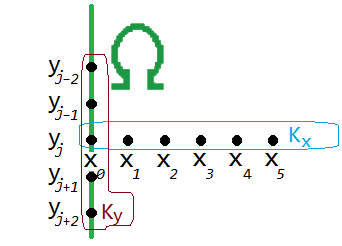
\includegraphics[width=\linewidth]{LeftBoundary.png}
		\centerline{\ref{fig:LeftBoundary}a) $K_x[0,1,2,3,4,5]$ }
	\end{minipage}	
	\begin{minipage}[b]{0.33\linewidth}
		\raggedright
		 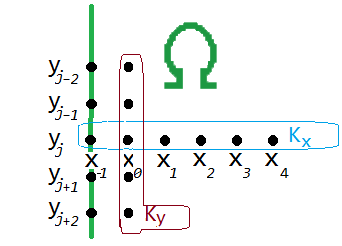
\includegraphics[width=\linewidth]{LeftBoundaryB.png}
		\centerline{\ref{fig:LeftBoundary}б) $K_x[-1,0,1,2,3,4]$ }
	\end{minipage}

	\caption{Шаблони с $O(h^4)$ апроксимация при имплементация на $\Delta_{h,4}$ оператора по лявата граница на областта.}
	\label{fig:LeftBoundary}
\end{figure}

Първият ред се извежда, използвайки следното условие: $\Delta u(x_0, y, t) = 0$ върху лявата граница на областта. Kрайната разлика напред на втората производна по $x$, във възела $(x_0, y_j)$, е нула и от тук се изразява стойността на последния възел спрямо останалите. Полученият израз се замества в крайната разлика по $x$ за възела $(x_1, y_j)$, което намалява броя на използваните точки с една. Тази процедура е описана подробно по-надолу. 

Крайната разлика напред $K_x[0,1,2,3,4,5]$ за втората производна по $x$ и централна крайна разлика $K_y[-2,-1,0,1,2]$ за втората производна по $y$ са представени на Фигура \ref{fig:LeftBoundary}a. С вектора в квадратните скоби на крайните разлики $K_x$ и $K_y$ се обозначава релативната позиция на използваните възли. Резултатът от производните пресметнати посредством $K_x$ и $K_y$ се отнася за възела, обозначен с нула. Понеже $u(x_0, y, t) = 0$ следва, че събираемите от $K_y[-2,-1,0,1,2]$, заедно с първия елемент от $K_x[0,1,2,3,4,5]$, са нула. Последното важи за всяка крайна разлика $K_y$ с точки върху границата $\partial \Omega_h$. Ако означим с $\bar c_0, \bar c_1, .., \bar c_5$ теглата на крайната разлика напред $K_x[0,1,2,3,4,5]$ (от Фигура \ref{fig:LeftBoundary}a) и с $\bar d_0, \bar d_1,.., \bar d_5$ теглата на крайната разлика $K_x[-1,0,1,2,3,4]$ (от Фигура \ref{fig:LeftBoundary}б), се получава, че:
\begin{align}
\sum\limits_{i=0}^{5} \bar c_i u(x+ih, y_j) = \sum\limits_{i=1}^{5} \bar c_i u(x+ih, y_j) = 0 &  \quad | \frac{\bar d_5}{\bar c_5} \nonumber\\
\bar d_5 u(x+5h, y_j) = -\sum\limits_{i=1}^{4} \bar c_i u(x+ih, y_j) & \nonumber
\end{align}
Последният член $u(x+5h, y_j)$ от $K_x[0,1,2,3,4,5]$ е изразен чрез останалите и може да се замести в $K_x[-1,0,1,2,3,4]$ както следва:
\begin{align}\label{fdResult}
&\sum\limits_{i=0}^{5} \bar d_i u(x+ih, y_j) = \sum\limits_{i=1}^{5} \bar d_i u(x+ih, y_j)  =  \\
&\sum\limits_{i=1}^{4} \left( \bar d_i u(x+ih, y_j) - \bar c_i u(x+ih, y_j) \right) = \sum\limits_{i=1}^{4} \left( \bar d_i - \frac{\bar d_5}{\bar c_5} \bar c_i \right) u(x+ih, y_j) \nonumber
\end{align}
Понеже $K_x[0,1,2,3,4,5]$ и $K_x[-1,0,1,2,3,4]$ са крайни разлики, апроксимиращи втора производна с грешка $O(h^4)$ (\cite{forn}), то полученият резултат \rf{fdResult} за възела от Фигура \ref{fig:LeftBoundary}б е със същата грешка $O(h^4)$. Теглата $\bar c_i$ и $\bar d_i$ при $p=4$ са дефинирани както следва (\cite{forn}):
\begin{align}
&\bar c_i, i = 0,..,5 \iff \frac{15}{4}, -\frac{77}{6}, \frac{107}{6}, -13, \frac{61}{12}, -\frac{5}{6} \\
&\bar d_i, i = 0,..,5 \iff \frac{5}{6}, -\frac{5}{4}, -\frac{1}{3}, \frac{7}{6}, -\frac{1}{2}, \frac{1}{12} 
\end{align}
и след като се заместят в \rf{fdResult}, се получават коефициентите от първия ред на матрицата $\Delta_{h,4,x}$. При последния ред се прилагат аналогични разсъждения върху дясната граница на областта, но вече се използва крайна разлика назад $K_x[-4,-3,-2,-1,0]$ за втората производна по $x$, при пресмятането на дискретния Лапласиан. 

Аналогични разсъждения се прилагат за горната и долната граници на областта при другата матрица $\Delta_{h,4,y}$, която се използва за изчисляването на втората производна по $y$ и затова нейната структура е същата.

При $p=6$ матрицата $\Delta_{h,6,x}$ има следния вид:
\[
\frac{1}{h^2}
\begin{bmatrix}
   -\frac{327}{140}	& \frac{191}{168}	&   \frac{167}{1134}	& -\frac{1}{7}    		 & \frac{19}{420}	& -\frac{77}{13331}   &    0      	   	&   \dots           & 0    \\
    \frac{54}{35}    	&-\frac{235}{84}   	&    \frac{884}{567}    &-\frac{5}{28}  	 	& \frac{2}{105}		&  -\frac{11}{11340}	 &   0      	   	&   \dots	       & \vdots  \\
    -\frac{3}{20}		& \frac{3}{2}         	& -\frac{49}{18} 	&  \frac{3}{2}		&  -\frac{3}{20}    	 &   \frac{1}{90}    	 &  0			&     \dots         &\vdots    \\
    \frac{1}{90}		& -\frac{3}{20}		& \frac{3}{2}         	& -\frac{49}{18} 	&  \frac{3}{2}		&  -\frac{3}{20}    	 &   \frac{1}{90} &     \dots         &\vdots    \\
        0           		& \ddots        		&         \ddots           	& \ddots        		&    \ddots   		&   \ddots      		 &     \ddots    	&  \ddots          &    0 \\	
\\
   \vdots      		&            		 	&    	0	      		& \frac{1}{90}		& -\frac{3}{20}		& \frac{3}{2}         	& -\frac{49}{18}	&  \frac{3}{2}  &  -\frac{3}{20} \\
    0      			&              	 	&    0      		&   -\frac{11}{11340}	 	&    \frac{2}{105} 	&  -\frac{5}{28} 	& \frac{884}{567} &-\frac{235}{84} &  \frac{54}{35}\\
    0              	& 	          		&    0              	&  -\frac{77}{13331}    		&  \frac{19}{420}&-\frac{1}{7}	 &  \frac{167}{1134} 	& \frac{191}{168}  &  -\frac{327}{140}\\
\end{bmatrix}
\]
Третият и предпредпоследният ред на матрицата $\Delta_{h,6,x}$ сa следствие от факта, че $u \in W^1_2(\Omega)$ и съответно $u(x_0, y_j, t_k) =$ $u(x_{N_x}, y_j, t_k) = 0$ както е при $O(h^2)$ апроксимацията. 

\begin{figure}%{r}{50mm}
	\begin{minipage}[b]{0.32\linewidth}
		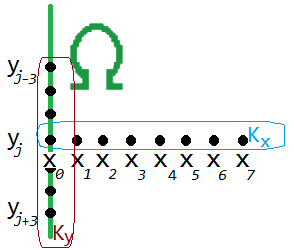
\includegraphics[width=\linewidth]{LeftBoundaryC.png}
		\centerline{\ref{fig:LeftBoundary6}a) }
		\centerline{ $K_x[0,1,2,3,4,5,6,7]$ }
	\end{minipage}	
	\begin{minipage}[b]{0.32\linewidth}
		 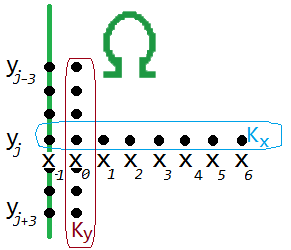
\includegraphics[width=\linewidth]{LeftBoundaryD.png}
		\centerline{\ref{fig:LeftBoundary6}б)  }
		\centerline{ $K_x[-1,0,1,2,3,4,5,6]$ }
	\end{minipage}
	\begin{minipage}[b]{0.32\linewidth}
		 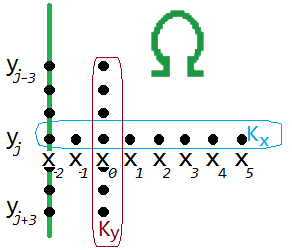
\includegraphics[width=\linewidth]{LeftBoundaryE.png}
		\centerline{\ref{fig:LeftBoundary6}с)  }
		\centerline{$K_x[-2,-1,0,1,2,3,4,5]$ }
	\end{minipage}

	\caption{Шаблони с $O(h^6)$ апроксимация при имплементация на $\Delta_{h,6}$ оператора по лявата граница на областта.}
	\label{fig:LeftBoundary6}
\end{figure}

Първият ред се извежда, използвайки следното условие: $\Delta u(x_0, y, t) = 0$ върху лявата граница на областта. Kрайната разлика напред на втората производна по $x$, във възела $(x_0, y_j)$, е нула и от тук се изразява стойността на последния възел спрямо останалите. Полученият израз се замества в крайната разлика по $x$ за възлите $(x_1, y_j)$ и $(x_2, y_j)$, което намалява броя на използваните точки с една. Тази процедура е описана подробно по-надолу. 

Крайната разлика напред $K_x[0,1,2,3,4,5,6,7]$ за втората производна по $x$ и централната крайна разлика $K_y[-3,-2,-1,0,1,2,3]$ за втората производна по $y$ са представени на Фигура \ref{fig:LeftBoundary6}а. Понеже $u(x_0, y, t) = 0$ следва, че събираемите от $K_y[-3,-2,-1,0,1,2,3]$, заедно с първия елемент от $K_x[0,1,2,3,4,5,6,7]$, са нула. Като последното важи за всяка крайна разлика $K_y$ с точки върху границата $\partial \Omega$. Ако означим с $\bar c_0, \bar c_1, .., \bar c_7$ теглата на крайната разлика напред $K_x[0,1,2,3,4,5,6,7]$ (от Фигура \ref{fig:LeftBoundary6}а) и с $\bar d_0, \bar d_1,.., \bar d_7$ теглата на крайната разлика $K_x[-1,0,1,2,3,4,5,6]$ (от Фигура \ref{fig:LeftBoundary6}б) се получава че:
\begin{align}\label{deltaOh6Zero}
\sum\limits_{i=0}^{7} \bar c_i u(x+ih, y_j) = \sum\limits_{i=1}^{7} \bar c_i u(x+ih, y_j) = 0 &  \quad | \frac{\bar d_7}{\bar c_7} \nonumber\\
\bar d_7 u(x+7h, y_j) = -\sum\limits_{i=1}^{6} \bar c_i u(x+ih, y_j) & 
\end{align}
Последният член $u(x+7h, y_j)$ от $K_x[0,1,2,3,4,5,6,7]$ е изразен чрез останалите и може да се замести в $K_x[-1,0,1,2,3,4,6]$ както следва:
\begin{align}\label{fdResultOh6}
&\sum\limits_{i=0}^{7} \bar d_i u(x+ih, y_j) = \sum\limits_{i=1}^{7} \bar d_i u(x+ih, y_j)  =  \\
&\sum\limits_{i=1}^{6} \left( \bar d_i u(x+ih, y_j) - \bar c_i u(x+ih, y_j) \right) = \sum\limits_{i=1}^{6} \left( \bar d_i - \frac{\bar d_7}{\bar c_7} \bar c_i \right) u(x+ih, y_j) \nonumber
\end{align}
Понеже $K_x[0,1,2,3,4,5,6,7]$ и $K_x[-1,0,1,2,3,4,5,6]$ са крайни разлики, апроксимиращи втора производна с грешка $O(h^6)$ (\cite{forn}), то полученият резултат \rf{fdResultOh6} за възела от Фигура \ref{fig:LeftBoundary6}б е със същата грешка $O(h^6)$. Теглата $\bar c_i$ и $\bar d_i$ при $p=6$ са дефинирани както следва (\cite{forn}):
\begin{align}
&\bar c_i, i = 0,..,7 \iff \frac{469}{90}, -\frac{223}{10}, \frac{879}{20}, -\frac{949}{18}, 41, -\frac{201}{10}, \frac{1019}{180}, -\frac{7}{10} \\
&\bar d_i, i = 0,..,7 \iff \frac{7}{10}, -\frac{7}{18}, -\frac{27}{10}, \frac{19}{4}, -\frac{67}{18}, \frac{9}{5}, -\frac{1}{2}, \frac{11}{180}
\end{align}
и след като се заместят в \rf{fdResultOh6}, се получават коефициентите от първия ред на матрицата $\Delta_{h,6,x}$. 

Ако пък с $\bar d_0, \bar d_1, .., \bar d_7$ се означат теглата в $K_x[-2,-1,0,1,2,3,4,5]$ (от Фигура \ref{fig:LeftBoundary6}с) и се използва резултата от \rf{deltaOh6Zero}, то тогава в \rf{fdResultOh6} се получават коефициентите от втория ред в $\Delta_{h,6,x}$, които са за възела от Фигура \ref{fig:LeftBoundary6}с). Коефициентите при $K_x[-2,-1,0,1,2,3,4,5]$ са:
\begin{align}
&\bar d_i, i = 0,..,7 \iff -\frac{11}{180}, \frac{107}{90}, -\frac{21}{10}, \frac{13}{18}, \frac{17}{36}, -\frac{3}{10}, \frac{4}{45}, -\frac{1}{90}
\end{align}
За да се построи долната дясна част на матрцата, се подхожда както до сега при горната лява част. Аналогични разсъждения се прилагат за горната и долната граници на областта при другата матрица $\Delta_{h,6,y}$, която се използва за изчисляването на втората производна по $y$, където отново се получава същата структура.

\subsection{Симетрично гранично условие по абцисата и ординатата при елиптичната задача}\label{symBndHead}
Смяната на променливата $\tilde {\bar x } = -x$ в уравнение \rf{eq2} води до същото такова, т.е. то не се променя. Същото важи и за смяната $\tilde {\bar y } = -y$. Затова решенията от стационарната задача \rf{eq2} са симетрични по $x$ и $y$ осите. Това позволява да се търси решение само в първи квадрант $\omega := \{ (x,y) \in \Omega : x \geq 0, y \geq 0 \}$. Уловието на симетрия може да се построи посредством следния запис:
\begin{align}\label{funSpaceSym}
W^1_2(\omega) =\{ u : \Omega \rightarrow \RR : \nonumber \\ 
	                     u(x,y) = u(x,-y), u(x,y) = u(-x,y), \; u \in W^1_2(\Omega) \}
\end{align}
и в последствие уравнението \rf{eq2} ще се разглежда само в $\omega_h \in \Omega_h$. Дискретните оператори $\Delta_{h,p,x}$ и $\Delta_{h,p,y}$, дефинирани в секция \ref{zeroBndHead} ``Нулево гранично условие'', ще бъдат от помощ при построяването на $\Delta_{h,p,s,x}$ с размери $(N_x-1)/2 \times (N_x-1)/2$ и $\Delta_{h,p,s,y}$ с размери $(N_y-1)/2\times(N_y-1)/2$, описващи симетричното условие по абцисата и ординатата в $\omega_h$:
\be\label{PsnDiscretSym}
\Delta_{h,p,s}(v^{(k)}) := \Delta_{h,p,s,x}  v^{(k)} + v^{(k)} (\Delta_{h,p,s,y})^T.
\ee
Структурата на матриците $\Delta_{h,p,s,x}$ и $\Delta_{h,p,s,y}$ се различава от $\Delta_{h,p,x}$ и $\Delta_{h,p,y}$ само в първите $i$ редове (при $p=2$ и $i=0$, при $p=4$ и $i=0,1$, при $p=6$ и $i=0,1,2$), където е приложено условието за симетрия. Останалите редове и ненулевите елементи спрямо главните им диагонали са едни и същи, защото апроксимират втора производна с един и същи ред на апроксимация $p$, и нулево гранично условие по границите $x=L_x$ и $y=L_y$. Така, при $p=2$ се получава, че 
\[
\Delta_{h,2,s,x} = \frac{1}{h^2}
\begin{bmatrix}
    -2	       & 2        &     \dots   &   \dots        & 0   \\
    1               & -2            &   1           &   0               & \vdots    \\
        0           & \ddots        &    \ddots    &   \ddots       &  0 \\ 
    \vdots       &     0            &  1     	& -2    	   & 1 \\
    0               & \dots          &  \dots         & 1  	   & -2 \\
\end{bmatrix}
,
\]
защото $u \in W^1_2(\omega)$ и $u(x_1, y_j) = u(x_{-1}, y_j)$ и следователно $u(x_1, y_j) + u(x_{-1}, y_j) = 2 u(x_1, y_j)$. По същия начин, но с различна големина, изглежда и матрицата $\Delta_{h,p,s,y}$, защото $u \in W^1_2$ и $u(x_i, y_1) = u(x_i, y_{-1})$.  

При $p=4$ имаме, че 
\[
\Delta_{h,4,s,x} = \frac{1}{h^2}
\begin{bmatrix}
     -\frac{5}{2}	& \frac{8}{3}       & -\frac{1}{6}	&    0     			&    \dots      	   &   0           & 0    \\
    \frac{4}{3}          &-\frac{31}{12}    	& \frac{4}{3}	&   -\frac{1}{12}	  	&   \dots      	  &   0	           & \vdots  \\
    -\frac{1}{12}	& \frac{4}{3}         	& -\frac{5}{2}	&  \frac{4}{3}    	 &   -\frac{1}{12}	  &      0           &\vdots    \\
        0           		& \ddots        	&    \ddots   		 &   \ddots      	 &     \ddots      	  &  \ddots        &    0 \\	
\\
   \vdots      		 & 0           		 &  -\frac{1}{12}	& \frac{4}{3}    	& -\frac{5}{2}	&  \frac{4}{3}   &   -\frac{1}{12} \\
    0      		 &  \dots           	 &   0     		& -\frac{1}{12} 	 & \frac{4}{3} 	 & -\frac{5}{2}  &  \frac{4}{3}\\
    0              		 & \dots          	&  0              		 &\frac{1}{120} 	 &  -\frac{2}{15} 	& \frac{29}{20} & -\frac{38}{15}\\
\end{bmatrix}
\]
Вторият ред на матрицата $\Delta_{h,4,s,x}$, който представя крайната разлика $K_x[-1,0,1,2]$, е изведен използвайки апроксимацията от 4ти ред в Таблица \ref{table:A00}
$$ -\frac{1}{12}, \frac{4}{3}, -\frac{5}{2},  \frac{4}{3}, -\frac{1}{12} $$ и условието, че
$$u(x_1, y_j) = u(x_{-1}, y_j).$$
Така централният възел е модифициран, първият е премахнат, а останалите са непроменени. 

За извеждането на първия ред в $\Delta_{h,4,s,x}$ за крайната разлика $K_x[0,1,2]$ се използват следните равенства
$$u(x_1, y_j) = u(x_{-1}, y_j), u(x_2, y_j) = u(x_{-2}, y_j)$$
и отново Таблица \ref{table:A00}.

Аналогични разсъждения се прилагат за границата, разположена върху ординатата при $\omega_h$ за другата матрица $\Delta_{h,4,s,y}$, която се използва за изчисляването на втората производна по $y$ и затова нейната структура е същата както при $\Delta_{h,4,s,x}$, но размерът ѝ е друг.

При $p=6$ матрицата $\Delta_{h,6,s,x}$ има следния вид:
\[
\frac{1}{h^2}
\begin{bmatrix}
   -\frac{49}{18}		& \frac{3}{1}			&   -\frac{3}{10}		& \frac{1}{45}    		 &  0					& 0	   					&    0      	   	&   \dots           & 0    \\
    \frac{3}{2}    	&-\frac{517}{180}    	&    \frac{68}{45}     & -\frac{3}{20}  	 		& \frac{1}{90} 		&  0					 &   0      	   	&   \dots	       & \vdots  \\
    -\frac{3}{20}		& \frac{68}{45}         	& -\frac{49}{18} 	&  \frac{3}{2}		&  -\frac{3}{20}    	 &   \frac{1}{90}    	 &  0			&     \dots         &\vdots    \\
    \frac{1}{90}		& -\frac{3}{20}		& \frac{3}{2}         	& -\frac{49}{18} 	&  \frac{3}{2}		&  -\frac{3}{20}    	 &   \frac{1}{90} &     \dots         &\vdots    \\
        0           		& \ddots        		&         \ddots           	& \ddots        		&    \ddots   		&   \ddots      		 &     \ddots    	&  \ddots          &    0 \\	
\\
   \vdots      		&            		 	&    	0	      		& \frac{1}{90}		& -\frac{3}{20}		& \frac{3}{2}         	& -\frac{49}{18}	&  \frac{3}{2}  &  -\frac{3}{20} \\
    0      			&              	 	&    0      		&   -\frac{11}{11340}	 	&    \frac{2}{105} 	&  -\frac{5}{28} 	& \frac{884}{567} &-\frac{235}{84} &  \frac{54}{35}\\
    0              	& 	          		&    0              	&  -\frac{77}{13331}    		&  \frac{19}{420}&-\frac{1}{7}	 &  \frac{167}{1134} 	& \frac{191}{168}  &  -\frac{327}{140}\\
\end{bmatrix}
\]
Третият ред на матрицата $\Delta_{h,6,s,x}$, който се отнася за крайната разлика 
$K_x[-2,$ $-1,0,1,2,3]$, се изразява от условието, че $u \in W^1_2(\omega)$ и съответно $u(x_1, y_j) = u(x_{-1}, y_j)$. Тук първият възел е премахнат, третият е модифициран, а останалите са непроменени. При втория ред на матрицата $\Delta_{h,6,s,x}$ ($K_x[-1,0,1,2,3]$) от условието за симетричност се използва, че
$u(x_1, y_j) = u(x_{-1}, y_j), u(x_2, y_j) = u(x_{-2}, y_j).$
Първите два възела се приспадат, съответно към петия и четвъртия, а останалите са непроменени. 
За първия ред ($K_x[0,1,2,3]$) симетрията се пада спрямо централния възел на крайната разлика и лесно се вижда, че
\begin{align}
\frac{1}{90}u(x_{-3}, y_j) +\frac{1}{90}u(x_3, y_j) = \frac{1}{45}u(x_3, y_j), \nonumber\\
-\frac{3}{20}u(x_{-2}, y_j) - \frac{3}{20}u(x_2, y_j) = -\frac{3}{10}u(x_2, y_j), \nonumber\\
\frac{3}{2}u(x_{-1}, y_j) + \frac{3}{2}u(x_1, y_j) = \frac{3}{1}u(x_1, y_j). \nonumber
\end{align}
Аналогични разсъждения се прилагат за границата разположена върху ординатата при $\omega_h$ за другата матрица $\Delta_{h,6,s,y} $, която се използва за изчисляването на втората производна по $y$ и затова нейната структура е същата както при $\Delta_{h,6,s,x}$, но размерът ѝ е друг. 

\subsection{Инструменти, използвани при числените резултати}\label{Instruments}

Редът на сходимост на изследваните крайни разлики и развития в ред на Тейлор са получени посредством правилото на Рунге:
\begin{equation}\label{Runge}
\xi = ln  \frac{\Vert u_{h,\tau} - u_{(h/2,\tau/2)} \Vert_\kappa } {\Vert  u_{(h/2,\tau/2)} - u_{(h/4,\tau/4)} \Vert_\kappa  } / ln(2),
\end{equation}
когато не е известно аналитично решение на уравнението, а нормата $\kappa$ е подходящо подбрана. Тук $u_{h,\tau}$ е решението получено при стъпки $h$ и $\tau$. В настоящата работа за $\kappa$ са използвани $L_2$ и $L_\infty$ норми:
\begin{align*}
\Vert u_{h,\tau} \Vert_{L_2} = \sqrt{ h^2 \sum_{i=1}^{N_x-1} \sum_{j=1}^{N_y-1}  (u_{i,j})^2 } \\
\Vert u_{h,\tau} \Vert_{L_\infty} = \max_{i,j}(|u_{i,j}|), \; i=1,..,N_x, j=1,..,N_y
\end{align*}
Формула \rf{Runge} е използвана и при изчислението на сходимостта на дискретната енергията върху три вложени мрежи с размери $[0:\tau:T]$, $[0:\tau/2:T]$ и $[0:\tau/4:T]$. За простота в долните Tаблици \ref{tab:a}, \ref{tab:fourth-der}, \ref{tableC} и \ref{tableA} се използва следното означение за грешката в решението:
$$\Vert \bar E_i \Vert_\kappa =  \Vert u_{h,\tau} - u_{(h/2,\tau/2)} \Vert_\kappa.$$ 
При Енергията съответно в Таблици \ref{tableD} и \ref{tableB} се използва следния запис
$$\Vert \bar{\bar{ E_i}} \Vert_\kappa=  \Vert E(u_{h,\tau}) - E(u_{(h/2,\tau/2)}) \Vert_\kappa,$$ 
където $E(u_{h,\tau})$ е функционала на енергията, пресметнат използвайки численото решение $u_{h,\tau}$.
Числените резултати, получени при намиране на решенията на елиптичната и хиперболичната задачи, са извършени при $\alpha = 1$ и следните три случая (виж Таблица \ref{tableP}) $\beta = 3$, $c=0.45$, $\beta = 1$, $c=0.9$ и $\beta = 3$, $c=0.3$
\begin{table}
\centering
\small
		\begin{tabular}{||c|l|l|l|l|l|l|l||}
			\hline
			\hline
          &    $\beta$, $c$ 	 & $O(|h|^p+\tau^p)$   &      $h$       	& $L_x$,$L_y$   	&  $T$    	& Гр. Усл.  \\
   			\hline 
			\hline
Тест 1  &      $\beta = 3$   &      $p=2, 4, 6$    	&    $h=0.2,$       	& $L_x = 30$     	&    10    	&    нулево;  \\
          &      $c=0.45$       &                           	&    $ 0.1, 0.05$   	& $L_y=27	$    	&        		&     ненулево 		\\
	   		\hline
			\hline 
Тест 2	&      $\beta = 1$	&      $p=2, 4, 6$    	&     $h=0.4,$      	& $L_x = 128$    &   10    	&   нулево;  \\
           &      $c=0.9$      	&                       		&      $0.2, 0.1$     & $L_y=58$         	&          		&   ненулево   \\
	   		\hline
			\hline 
Тест 3	&      $\beta = 3$	&      $p=4, 6$    	&     $h=0.4,$      	& $L_x = 50$    &   10    	&   нулево  \\
           &      $c=0.3$      	&                       		&      $0.2, 0.1$     & $L_y=50$         	&          		&      \\
	   \hline
			\hline 
		\end{tabular}
\caption{Параметрична таблица с описание на числените тестове. Нулевото гранично условие е описано в Глава \ref{zeroBndHead}, а ненулевото в Глава \ref{symBndHead}.}
\label{tableP}
\end{table}
с последващи уточнения. Първо, Консервативната схема е имплементирана само при $p=2$. Второ, при хиперболичната задача стъпката по времето е $\tau = h/2$. Трето, при решаването на елиптичната задача се използва мрежата $\omega_h \subset \Omega_h$ само в първи квадрант, като там се прилага симетричното гранично условие по абцисата и ординатата, докато хиперболичната задача се разглежда в цялата област $\Omega_h$ и там не се използва симетричното, а само нулевото или ненулевото гранично условие, дефинирани съответно в глави \ref{zeroBndHead} ``Нулево гранично условие'' и \ref{symBndHead} ``Ново гранично условие за двумерното елиптично уравнение \rf{eq3}''.

\subsection{Квадратурни формули за пресмятане на двумерни интеграли}\label{quadratureFormulas}
Непрекъснатата хиперболична задача \rf{problemVC} притежава следните инварианти: маса и енергия, дефинирани съответно както следва:
\begin{equation}\label{intM}
M(u(x,y,t)):=\int_{\RR^2} u(x,y,t)dx dy,
\end{equation}

\begin{align}\label{ex-en}
&E(u(x,y,t)):= \nonumber\\ 
&\beta \int_{\RR^2} u_t(x,y,t) \: \left(A^{-1}+E_1\right)u_t(x,y,t) dxdy+
\beta \int_{\RR^2} u^2(x,y,t) dxdy \nonumber\\
&+\int_{\RR^2}u(x,y,t) \left(A u(x,y,t)\right) dxdy - \frac{2 \alpha \beta}{3} \int_{\RR^2} u^3(x,y,t) dxdy,
\end{align}
където $Au=-\Delta u$ действа във функционалното пространство $W^1_2(\Omega)$ от \rf{funSpace}. В \cite{ref1} е доказано, че масата и енергията се запазват във времето: 
$$M(u(x,y,t)) = M(u(x,y,0))  \text{ и } E(u(x,y,t)) = E(u(x,y,0)).$$
Нека да заменим оператора $Au=-\Delta u$ с неговия дискретен такъв $A_hu :=-\Delta_h u$, като използваме апроксимаций от различен ред - $O(|h|^2)$, $O(|h|^4)$, $O(|h|^6)$. За численото пресмятане на интегралите в \rf{intM} и \rf{ex-en} използваме следните квадратурни формули, които ще дефинираме за  интеграла 
\begin{equation}\label{int}
D(u(x,y))=\int_{a_1}^{b_1} \int_{a_2}^{b_2} u(x,y)dx dy
\end{equation}
върху областта $[a_1, b_1] \times [a_2, b_2]$, като е използвана следната мрежа:
$$x_i, ~i=0,1,...,N_x-1; \;x_0=a_1,~x_{N_x}=b_1, \;h_1=(b_1-a_1)/(N_x-1),$$
$$y_j, ~j=0,1,...,N_y-1; \; y_0=a_2,~y_{N_y}=b_2, \;h_2=(b_2-a_2)/(N_y-1).$$

\subsubsection{ 2Д формула на трапците с глобална грешка $O(|h_1|^2+|h_2|^2)$ }

Апроксимацията на интеграла \eqref{int} с грешка $O(|h_1|^2+|h_2|^2)$ е

\begin{align}\label{quadr2}
D_h(u_{i,j}) =& \sum_{i=1}^{N_x-1} \sum_{j=1}^{N_y-1} h_1 h_2 u_{i,j}
+\frac{h_1}{2}\sum_{i=0} \sum_{j=1}^{N_y-1} h_2 u_{i,j}
+\frac{h_1}{2}\sum_{i=N_x} \sum_{j=1}^{N_y-1} h_2 u_{i,j} \nonumber\\
+&\frac{h_2}{2}\sum_{j=0} \sum_{i=1}^{N_x-1} h_1 u_{i,j}
+\frac{h_2}{2}\sum_{j=N_y} \sum_{i=1}^{N_x-1} h_1 u_{i,j}
\nonumber\\
+&\frac{1}{4}h_1 h_2 \left(u_{0,0}+u_{N_x,0}+u_{N_x,N_y}+u_{0,N_y}
\right).
\end{align}

\subsubsection{ 2Д правило на Симпсън с глобална грешка $O(|h_1|^4+|h_2|^4)$}

Нека да приемем, че $N_x=2k$, $N_y=2 l$. Така, за всяко $m=0,1,2,\cdots N_y$ пресмятаме, че

$$D_m= \frac{h_1 }{3} 
\left\{ u_{0,m}+u_{N_x,m}+ 4 \sum_{i=1}^{\frac{N_x}{2}}   u_{2i-1,m}
 +2 \sum_{i=1}^{\frac{N_x}{2}-1} u_{2i,m} \right\}.$$


От последната формула получаваме

\begin{equation}\label{quadr4}
D_h(u_{i,j}) =\frac{h_2 }{3} 
\left\{ D_{0}+D_{N_y}+ 4 \sum_{j=1}^{\frac{N_y}{2}}   D_{2j-1}
 +2 \sum_{j=1}^{{\frac{N_y}{2}}-1} D_{2j} \right\}
\end{equation}
апроксимацията на интеграла \eqref{int} с глобална грешка $O(|h_1|^4+|h_2|^4)$.


\subsubsection{ 2Д правило на Буул с глобална грешка $O(|h_1|^6+|h_2|^6)$}

Нека да приемем, че $N_x=4k$, $N_y=4 l$. Така, за всяко $m=0,1,2,\cdots N_y$ пресмятаме, че

\begin{align*}
D_m =& \frac{2h_1}{45} 
\left\{
7u_{0,m}+7u_{N_x,m}+32 \sum_{i=1}^{\frac{N_x}{2}}u_{2i-1,m}
+12\sum_{i=1}^{\frac{N_x}{4}}u_{4i-2,m}
+14 \sum_{i=1}^{\frac{N_x}{4}-1}u_{4i,m}
\right\}.
\end{align*}

Тогава формула \eqref{quadr6-2D} е апроксимацията на интеграла \eqref{int} с глобална грешка $O(|h_1|^6+|h_2|^6)$ (\cite{boole}).

\begin{align}\label{quadr6-2D}
&D_h(u_{i,j})  =
\frac{2h_2}{45} 
\left\{
7D_{0}+7D_{N_y}+32 \sum_{j=1}^{\frac{N_y}{2}}D_{2j-1}
+12\sum_{j=1}^{\frac{N_y}{4}}D_{4j-2}
+14 \sum_{j=1}^{\frac{N_y}{4}-1}D_{4j}
\right\}.
\end{align}

\subsection{Бърз директен метод за обръщане на двумерния дискретен оператор на Лаплас (Fast Poisson Solvers) }\label{FPS}
Нека е дадена следната задача:
\be\label{PoissonEq}
-\Delta v = f
\ee
дефинирана в областта $\Omega$ с хомогенни гранични условия $v \big|_{\partial\Omega} = 0$. Дискретната версия на \rf{PoissonEq} използвайки \rf{DeltaH} има вида:
\be\label{PsnDiscret}
-\Delta_{h,p,x}  V_h - V_h (\Delta_{h,p,y})^T = F_h,
\ee
където $V_h, F_h$ са двумерни матрици с елементи съответно $v(x_i,y_j)$ и  $f(x_i,y_j)$, и една и съща големина $(N_x-2)\times(N_y-2)$. Дискретните функции $V_h, F_h$ представят непрекъснатите такива $v, f$ ограничени върху мрежата $\Omega_h$, т.е. $V_h = v(\Omega_h)$ и $F_h = f(\Omega_h)$ (виж Фигура \ref{fig:FPSexplained}).
\begin{figure}[ht]
     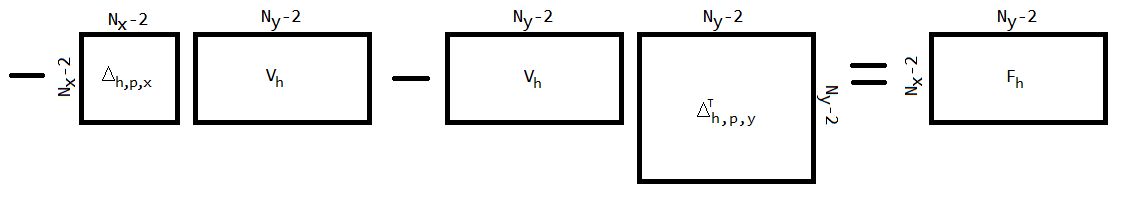
\includegraphics[width=\linewidth]{FPSExplained.png}
	\caption{Дискретното уравнение на Лаплас \rf{PsnDiscret} в матричен вид}
	\label{fig:FPSexplained}
\end{figure}
\FloatBarrier
Този тип запис на задачата \rf{PoissonEq} е разгледан от Том Личи в \cite{ref34}, където областта е квадратна $L_x = L_y$ и са използвани централни крайни разлики от втори ред $p=2$ с нулево гранично условие в $\partial \Omega_h$. При $p=2$ операторите $\Delta_{h,2,x}$ и $\Delta_{h,2,y}$ са симетрични, което допълнително улеснява търсенето на решение на поставената задача. Настоящата глава се явява разширение на горепосочения труд при произволна правоъгълна област с размери $2L_x \times 2L_y$ и несиметрични крайни разлики по границата на областта, където се прилага нулево гранично условие. Т.е. в общия случай матриците $\Delta_{h,p,x}$ и $\Delta_{h,p,y}$ не са симетрични, както е описано в настоящата работа в глава \ref{zeroBndHead} ``Нулево гранично условие'' при $p>2$. 

Нека за матриците $(\Delta_{h,p,x})^T$ и $(\Delta_{h,p,y})^T$ имаме следните собствени стойности $\lambda_{x,i}$, $\lambda_{y,j}$ и собствени вектори $s_{x,i}$, $s_{y,j}$:
\begin{align}
S_x:=[s_{x,1},..,s_{x,N_x-2}],\\
D_x:= diag(\lambda_{x,1},..,\lambda_{x,N_x-2}),\\
S_y:=[s_{y,1},..,s_{y,N_y-2}],\\
D_y:= diag(\lambda_{x,1},..,\lambda_{x,N_y-2}).
\end{align}
Така се получава, че
\begin{align}\label{eigIdentity}
(\Delta_{h,p,x})^T  S_x = S_x  D_x\nonumber\\
(\Delta_{h,p,y})^T   S_y = S_y  D_y,
\end{align}
където $S_x, S_y$ се явяват матриците със собствени вектори и $D_x, D_y$ са диагоналните матрици със собствени стойности съответно на $(\Delta_{h,p,x})^T, (\Delta_{h,p,y})^T$. Последните са пресметнати, използвайки специализиран софтуер и библиотеки за работа с големи матрици. Ако положим
\be\label{subst}
X_h := ( S_x^T  V_h  S_y ) \quad \text{с размери} (N_x-2)\times(N_y-2),
\ee
и заместим в \rf{PsnDiscret}, се получава:
\be
-\Delta_{h,p,x}  (S_x^T)^{-1} X_h  S_y^{-1}  -(S_x^T)^{-1} X_h  S_y^{-1}  (\Delta_{h,p,y})^T = F_h.
\ee
Умножаваме от ляво и дясно с $ S_x^T  ( . )  S_y$:
\be\label{fpp1}
- S_x^T \Delta_{h,p,x} (S_x^T)^{-1} X_h -X_h  S_y^{-1}  \Delta_{h,p,x}^T  S_y = S_x^T  ( F_h )  S_y.
\ee
Изразът $S_x^T  \Delta_{h,p,x}$ има следното представяне
\be
S_x^T  \Delta_{h,p,x} = (\Delta_{h,p,x}^T  S_x)^T =^{\rf{eigIdentity}} (S_x  D_x)^T = D_x  S_x^T
\ee
Последното се замества в \rf{fpp1} и използвайки пак \rf{eigIdentity} извеждаме равенството
\be
- D_x  S_x^T (S_x^T)^{-1} X_h  -X_h  S_y^{-1}  S_y  D_y = S_x^T  F_h   S_y,
\ee
за което след опростяване получаваме:
\be\label{fpp2}
- D_x  X_h -X_h  D_y = S_x^T  F_h  S_y.
\ee
Уравнение \rf{fpp2} е еквивалентно на
\be\label{fpp3}
-X_{i,j} \lambda_{x,i} - \lambda_{y,j} X_{i,j} = b_{i,j}.
\ee
разписано по компоненти и така се получава, че
\be\label{fpp4}
X_{i,j} = - b_{i,j}/(\lambda_{x,i} + \lambda_{y,j} ),
\ee
където $X_h = (X_{i,j})$ и $S_y^T  F_h   S_x = (b_{i,j})$ и това важи за всяко $(i,j)$:
$$i = 1,..,N_x-2, \quad j = 1,..,N_y-2 $$
с уточнението че $i = 0,N_x-1$, $j = 0,N_y-1$ са граничните стойности които не присъстват експлицитно в уравненията, но са взети в предвид. Имайки $X_h$ лесно може да получим $V_h$  с обратната субституция на \rf{subst}, която е 
\be\label{substInv}
V_h = (S_x^T)^{-1}  X_h  S_y^{-1}.
\ee

Да разгледаме следната задача:
\be\label{PoissonEqExt}
v-\Delta v = f,
\ee
дефинирана в областта $\Omega$ с хомогенни гранични условия $v \big|_{\partial\Omega} = 0$. В този случай дискретната версия на \rf{PoissonEqExt} използвайки \rf{DeltaH} има вида:
\be\label{PsnDiscretExt}
V_h - \Delta_{h,p,x}  V_h - V_h  (\Delta_{h,p,y}) ^{T}  = F_h,
\ee
което е аналогично с \rf{PsnDiscret} и дефинициите, заложени там. Използвайки същите съждения от \rf{subst}-\rf{fpp4} лесно се получава, че:
\be\label{fpp4Ext}
X_{i,j} = - b_{i,j}/(\lambda_{x,i}  + \lambda_{x,j} -1)
\ee
за всяко $(i,j)$, $i = 1,..,N_x-2$, $j = 1,..,N_y-2 $.
\subsubsection{Изчислителната сложност}
Изчислителната сложност при обръщането на оператора на Лаплас по метода в предходната част се разделя на две части. \textbf{ Първата част (I)} е свързана с изчисляването на собствените стойности $D_x, D_y$ и вектори $S_x, S_y$ на двете матрици $(\Delta_{h,p,x})^T$ и $(\Delta_{h,p,y})^T$. Също така се включват и пресмятанията, необходими за получаването на обратните матрици $(S_x^T)^{-1}$ и $S_y^{-1}$. Сложността на тези две процедури се оценя на $O(N_x^3+N_y^3)$ (\cite{ref260}) и съответно на $O(N_x^{2.37}+N_y^{2.37})$ (\cite{ref27}). \textbf{Втората част (II)} е свързана предимно с умножение на неразредени матрици в дясната част на \rf{fpp2} и обратната субституция \rf{substInv}, като и в двата случая произведението се формира от три матрици  с големини както следва: първата - $(N_x-2) \times (N_x-2)$, втората (средната) - $(N_x-2) \times (N_y-2)$ и третата - $(N_y-2) \times (N_y-2)$. \textbf{Това води} до изчислителна сложност от порядък
\be\label{fpsComplex}
O(N_x N_y \bar{\epsilon}),
\ee
\textbf{където $\bar{\epsilon} \in (0, max(N_x, N_y))$ (\cite{ref26, ref27})}. В случая, когато областта е квадратна, $N_x = N_y$ се получава, че $\bar{\epsilon} = 0.37 N_x$, т.е. алгоритмичната сложност е $O(N_x^{2.37})$. При метода на Тейлор изчисленията, описани в (I), се правят еднократно и получените резултати се използват в частта (II), която се прави за всеки слой по времето, т.е. (II) и \rf{fpsComplex} са с по-голяма тежест. 

\subsubsection{Изчислителната сложност при факторизация на Холески}
Равенствата \rf{PsnDiscret} и \rf{PsnDiscretExt} използват матрици, не по големи от $max(N_x, N_y) \times max(N_x, N_y))$, което позволява една компактност относно компютърната памет. В противен случай, ако се се борави с едномерен вектор за неизвестната функция $u$ от типа $\bar {b}_{(j-1)N_x + i} := u_{i,j}$, то тогава дискретният оператор на Лаплас ще е матрица с големина $\RR^{N_x^2 N_y^2}$ и при обръщането ѝ $-\Delta_{h,p}^{-1}\bar {b}$ посредством факторизация на Холески ще изисква изчислителна сложност от минимум $O(N_x^2 N_y^2)$ операции, възползвайки се от лентовата ѝ структура. Тук напомняме, че стандартната операция по факторизация на Холески за неразредена (пълна) матрица с големина $\RR^{N_x^2 N_y^2}$ отнема $O(N_x^3 N_y^3)$ операции.

\newpage
\section{Формулировка и числено решение на двумерното стационарно уравнение на Бусинеск - Метод на простата итерация}\label{ellipticFormulation}
В Част \ref{simpleIteration} е описан методът на простата итерация за намиране на решението на двумерното стационарно уравнение на Бусинеск, както е описано в \cite{ref16}. Дефинирана е явна диференчна схема за частните диференциални уравнения \rf{eq5}, чието решение се схожда към численото такова на уравненията \rf{eq45}. Показани са два варианта за начални стойности, задаващи първата итерация. Описано е как се променя стъпката по времето и какъв е критерият за спиране на итерационния алгоритъм. В последствие са дефинирани алгоритмични стъпки, с които може да се възпроизведе целият итерационен процес и е изведена алгоритмичната сложност. Най-накрая са представени редът на сходимост от метода на простата итерация, в табличен вид заедно с графики, показващи формата на решението за параметрите, разгледани в Таблица \ref{tableP}. 

В следващия Раздел \ref{resultsElliptic} са направени два числени теста при параметри $\beta = 3, c=0.45$ и $\beta = 1, c=0.9$, където $\beta = \beta_1/\beta_2$. За тези примери са показани следните резултати. Първо, резидуалът $R$ от последната итерация е представен в серия от графики. Второ, показано е, че четвъртите производни на решението, които са пресметнати числено, са сходящи по правилото на Рунге \rf{Runge}. Трето,  потвърдени са характерните свойства на получените решения за различни стойности на параметрите $\beta$ и $c$, които са представени първоначално в \cite{ref117,ref116} като например зависимостта на формата на вълната от скоростта $c$ и дисперсията $\beta$ и асимптотичното поведение $\frac{1}{x^2 + y^2}$ на безкрайност. 

Най-накрая, решението от последната итерация на числения метод, при $p=6$ е сравнено с ``best-fit'' апроксимационните формули от \cite{ref15}. Това сравнение все още липсва в литературата. Тук показваме съществени различия с ``best-fit'' формулите и считаме, че това е важен елемент и повратна точка в изследването на хиперболичната задача \rf{eq1}-\rf{eq11}. 

Част \ref{newBndHead} се занимава с едно ново гранично условие за елиптичната задача. Разгледана е асимптотиката на всеки един от членовете в стационарното уравнение на Бусинеск \rf{eq3}. В серия от числени експерименти при $\beta=1,3,5$, $c=0.17$ и при $\beta=1$, $c=0.1, 0.5, 0.9$ е показано, че асимптотиката на членовете с четвърти производни и нелинейните такива 
$$- v_{xxxx}, \;  - (2-\beta c^2)v_{xxyy},  \;  - (1-\beta c^2)v_{yyyy}, \;  - \alpha \beta (v^2)_{xx}, \; - \alpha \beta (v^2)_{yy}$$
е от порядък $O(r^{-6})$, а на членовете с втори производни 
$$\beta v_{xx}, \; \beta (1-c^2) v_{yy}$$
 е от порядък $O(r^{-4})$. Използвайки тази зависимост, членовете с асимптотика $O(r^{-6})$ в \rf{eq3} са пренебрегнати. Това ни помага да изведем явна формула
\be
\tilde v(x, y) = \mu_v \frac{ (1-c^2) x^2 - y^2 }{ ((1-c^2) x^2 + y^2)^2 }.
\ee
при $\sqrt{x^2+y^2} \rightarrow \infty$.
Последната формула е валидирана с помощта на два числени теста. При първият експеримент разглеждаме поведението на решението по границата, когато размерите на дискретната област $\Omega_h$ нарастват - $L_x = L_y = 20, 40, 80, 160$. При вторият тест разглеждаме поведението на функцията $\widehat v$ и нейната асимптотика по $x,y$ осите.

\subsection{Метод на простата итерация за числено решаване на стационарното Парадигматично уравнение на Бусинеск \rf{eq45}}\label{simpleIteration}
Посредством смяната на променливите $x=\sqrt\beta_1 { \overline x}$, $y=\sqrt\beta_1 { \overline y}$, $U(x,y)= v({ \overline x},{ \overline y} )$ уравнение 
\rf{eq2} добива следната форма
 \begin{align}\label{eq3}
&c^2 \beta (E_1- \Delta) v_{{\overline y}{\overline y}} = \beta \Delta v - \Delta^2 v - \beta \Delta f(v), \\ 
&v(\overline x, \overline y) \rightarrow 0,  \Delta v(\overline x, \overline y) \rightarrow 0 ,  \quad \text{за}  \sqrt{\overline x^2 + \overline y^2} \rightarrow \infty, \nonumber
\end{align}
взимайки предвид граничното условие от \rf{eq1}-\rf{eq11} и $\beta = \beta_1 / \beta_2$. Решението $v$ на \rf{eq3} заедно с неговите производни клони към нула, когато $|{\overline x}^2 +{\overline y}^2|\rightarrow \infty$. В тъждеството \rf{eq3}, производните от четвърти ред
\be
v_{{\overline x}{\overline x}{\overline x}{\overline x}} + (2-c^2\beta)v_{{\overline x}{\overline x}{\overline y}{\overline y}} + (1-c^2\beta) v_{{\overline y}{\overline y}{\overline y}{\overline y}}
\ee
образуват елиптично уравнение от четвърти ред, когато е изпълнено, че $c^2 < 1/\beta$, а производните от втори ред 
\be
-\beta v_{{\overline x}{\overline x}} - \beta (1-c^2)v_{{\overline y}{\overline y}} 
\ee
образуват елиптично уравнение от втори ред, когато е валидно, че $c^2 < 1$. Следователно уравнение \rf{eq3} е елиптично, когато горните две условия са изпълнени, т.е. $c^2 < \min(1, 1/\beta)$. В настоящата работа се разглеждат единствено такива параметри $\beta$ и $c$, които удовлетворяват последното изискване. За улеснение навсякъде по-надолу в текста ще се използват отново старите означения $x,y$ вместо ${\overline x},{\overline y}$.

Равенството \rf{eq3} може да се преобразува в система от две елиптични уравнения от втори ред по различни начини. Очаквайки, че производните $v_{xx}$ по оста $x$ ще са по-малки по абсолютна стойност от производните $v_{yy}$ по $y$ оста (тъй като решението се движи по $y$), заместваме $v_{yy} = \Delta v- v_{xx}$ в \rf{eq3}. След като се добави допълнителна функция $w$, се получава система, еквивалентна на \rf{eq3}
\begin{equation}\label{eq4}
- (1- c^2 \beta) v_{yy} - v_{xx} + \beta (1-c^2) v - \alpha \beta v^2 = w, 
\end{equation}
\begin{equation}\label{eq44}
 - \Delta w = c^2 \beta v_{xx}. 
\end{equation}
Търсят се ненулеви решения на \rf{eq4},\rf{eq44} както е описано в \cite{ref117,ref116}: фиксира се стойността на неизвестната функция $v$ в нулата, $v(0,0)=\theta$ и се въвеждат две нови функции: $\widehat{v}=v/{\theta} $ и $\widehat{w}=w/{\theta} $. Следователно $\widehat{v}(0,0)=1$ и 
\begin{equation}\label{eq45}
\begin{split}
 &- (1 - c^2 \beta) \widehat{v}_{yy} -\widehat{v}_{xx} + \beta (1-c^2) \widehat{v} - \alpha \beta \theta \widehat{v}^2 = \widehat{w}, \\
 &- \Delta \widehat{w} =  c^2 \beta \widehat{v}_{xx}.
\end{split}
\end{equation}
Стойността на $\theta$ се намира, използвайки следната зависимост
\begin{equation}\label{eqtheta}
\theta = \frac{ (1-c^2 \beta) \widehat{v}_{yy} + \widehat{v}_{xx} - \beta (1-c^2) \widehat{v} +\widehat{w}}{\alpha \beta \widehat{v}^2 } |_{x=0,y=0}.
\end{equation}
Численото решение на системата \rf{eq45} се намира чрез метода на простата итерация като изкуствено се добавят производни по времето както следва:
\begin{align}\label{eq5}
\begin{split}
 &\frac {\partial \widehat{v}}{\partial t} - (1 - c^2 \beta) \widehat{v}_{yy} -\widehat{v}_{xx} + \beta (1-c^2) \widehat{v} - \alpha \beta \theta \widehat{v}^2 = \widehat{w}, \\
 &\frac {\partial \widehat{w}}{\partial t} - \Delta \widehat{w} =  c^2 \beta \widehat{v}_{xx}. 
\end{split}
\end{align}
По този начин стационарната система от двете уравнения \rf{eq45} се заменя с преходните във времето уравнения, дефинирани в \rf{eq5}, с условието, че решенията $\widehat{v}$ и $\widehat{w}$ клонят по времето към решенията на \rf{eq45}.

Поради симетрията на проблема ще се разглеждат решенията получени само в първи квадрант $\omega = [0,L_x] \times[0,L_y] \in \Omega$. Дискретизацията на тази област води до мрежата $\omega_h$ дефинирана по следния начин:
$$
\omega_h = \{(x_i,y_j): x_i = ih, y_j = jh, i = 0,\cdots ,(N_x-1)/2, j = 0,\cdots , (N_y-1)/2 \},
$$
където дискретната стъпка $h$ е същата както при $\Omega_h$ и $\omega_h \in \Omega_h$. Времевата област е дефинирана чрез интервала $[0, \widehat T]$ или просто $\widehat T$, като стъпката по времето $\tau$ варира в зависимост от големината на резидуала \rf{residual} на решението. Това спомага за автоматизиране на контрола върху грешката (от апроксимацията и изчисленията, но с условието, че методът на простата итерация е сходящ). Стойността на функцията $v$ в точка от мрежата $x_i,y_j,t_k$ е означена с $v_{i,j}^{(k)}$. 
Дискретизацията на пространствените производни в \rf{eq5} е направена посредством централните крайни разлики, дефинирани в \rf{fdx}, \rf{fdy} и описани в Таблица \ref{table:A00}. Грешката от апроксимацията при формули \rf{fdx} и \rf{fdy} е $O(h^p)$. Непрекъснатият оператор на Лаплас в \rf{eq5} е заместен с дискретния такъв $\Delta_{h,p} (v_{i,j}) = (v_{i,j})_{\widehat{xx},p} + (v_{i,j})_{\widehat{yy},p}$ за $p=2,4,6$. Това води до по-висок ред на сходимост на метода при условие, че решението е достатъчно гладко. По този начин се получават по-точни решения върху по-едра мрежа. 
\par
Явното правило на Ойлер е използвано за апроксимацията на нововъведените производни по времето. Нелинейните членове в \rf{eq3} се пресмятат на всеки слой по времето $t^{(k)}$. Така, численото решение на следващия слой по времето $t^{(k+1)}$ е пресметнато директно чрез $v_{i,j}^{(k)}$ на предходния слой $t^{(k)}$:
\begin{equation}\label{eq55}
\begin{split}
&\frac {\widehat{v}_{i,j}^{(k+1)}-\widehat{v}_{i,j}^{(k)}}{\tau}- (1-c^2 \beta) \widehat{v}_{i,j,{\widehat{yy},p}}^{(k)} - \widehat{v}_{i,j,{\widehat{xx},p}}^{(k)} + \beta (1-c^2 ) \widehat{v}_{i,j}^{(k)} - \alpha \beta \theta (\widehat{v}_{i,j}^{(k)})^2 = \widehat{w}_{i,j}^{(k)}, \\
&\frac  {\widehat{w}_{i,j}^{(k+1)} -\widehat{w}_{i,j}^{(k)}} {\tau} - \Delta_{h,p} \widehat{w}_{i,j}^{(k)} =  c^2 \beta \widehat{v}_{i,j,{\widehat{xx},p}}^{(k)}.
\end{split}
\end{equation}
Този метод за решаване на уравненията \rf{eq45} е известен в литературата още като ``Метод на простата итерация" \cite{samarski}. С помощта на матриците $\Delta_{h,p,s,x}$ и $\Delta_{h,p,s,y}$, прилагаме нулево и симетрично гранични условия по границите на областта $\partial \omega$, запазвайки реда на използваната апроксимация $O(h^p)$ в \rf{eq55}. Така отчитайки \rf{PsnDiscretSym}, се получава следното матрично уравнение, допълващо \rf{eq55}, което отчита всички точки в $\omega_h$:
\begin{equation}\label{eq555}
\begin{split}
\frac {\widehat{v}^{(k+1)}-\widehat{v}^{(k)}}{\tau}- (1-c^2 \beta) \widehat{v}^{(k)}  (\Delta_{h,p,s,y})^T - \quad\quad\quad\;&\\
-\Delta_{h,p,s,x}  \widehat{v}^{(k)}+ \beta (1-c^2 ) \widehat{v}^{(k)} - \beta \theta f(\widehat{v}^{(k)}) &= \widehat{w}^{(k)}, \\
\frac  {\widehat{w}^{(k+1)} -\widehat{w}^{(k)}} {\tau} - \Delta_{h,p,s,x}  \widehat{w}^{(k)} - \widehat{w}^{(k)}  (\Delta_{h,p,s,y})^T &=  c^2 \beta \Delta_{h,p,s,x}  \widehat{v}^{(k)},
\end{split}
\end{equation}
където $\widehat{v}^{(k)}, \widehat{w}^{(k)}, \widehat{v}^{(k+1)}, \widehat{w}^{(k+1)}$ са матрици съответно с елементи ${v}_{i,j}^{(k)}$, ${w}_{i,j}^{(k)}$, ${v}_{i,j}^{(k+1)}$ и ${w}_{i,j}^{(k+1)}$ и една и съща големина $(N_x-1)/2 \times (N_y-1)/2$.
\subsubsection{Начални данни}
Цикличната процедура, описана в \rf{eq555}, се нуждае от начални стойности за функиите $\widehat{v},\widehat{w}$. Тук са разгледани два различни варианта. Оказва се, че те схождат към едно и също крайно решение. За всички разгледани параметрични случаи резидуала $R$, който е дефиниран в \rf{residual}, за началните данни (от първата итерация) е винаги по-голям от $1.0e-2$ и се извършват между $100,000$ и $10,000,000$ итерации докато се изпълни следното условие: $R<1.0e-9е$. 
 
В \textbf{първия случай} са избрани "best-fit" формулите от пертурбационното решение в \cite{ref15}. Върху тях се прилага същата смяна на променливите $x=\sqrt\beta_1 { \overline x}$, $y=\sqrt\beta_1 { \overline y}$, която е използвана в елиптичното уравнение \rf{eq3}. 

При \textbf{втория случай} е взето численото решение от задачата \rf{eq3} при $c=0$, което също е добро приближение и служи на начални стойности на \rf{eq555} дори когато търсим решение на последното при скорости близки до допустимия максимум $c \approx \min (1/ \sqrt{\beta},1)$, $c < \min (1/ \sqrt{\beta},1)$. Както е известно, при по-високи скорости "best-fit" формулите не апроксимират численото решение за елиптичната задача добре, поради естеството на получаването им.

При $c=0$ уравнение \rf{eq3} добива следния вид:
\be\label{eq3c0}
\Delta (\beta  v - \Delta v - \beta f(v)) = 0.
\ee
В частност, ако за уравнението 
\be\label{eq3c01}
\beta v - \Delta v - \beta f(v) = 0
\ee
съществува решение $\nu$, то също ще удовлетворява и \rf{eq3c0}.  В \cite{ref1c00} e показано, че този тип уравнение, с нелинейността зададена тук $f(v) = v^2$ и клонящо към нула на безкрайност, има най-много едно решение, което е радиално симетрично и монотонно намаляващо, когато се отдалечаваме от центъра. Това създава предпоставки да разгледаме тъждество \rf{eq3c01} в полярни координати, за да получим обикновено диференциално уравнение:
\begin{align}\label{eq3c02}
\beta v_{polar}(r)  - \frac{ \partial^2 v_{polar} } {\partial r^2}(r) - \frac{1}{r} \frac{ \partial v_{polar} } {\partial r}(r)  - \beta f(v_{polar}(r)) = 0, \nonumber \\
\frac{ \partial v_{polar} } {\partial r}(0) = 0, \quad v_{polar}(r) \rightarrow 0, \; \text{при} \; r \rightarrow \infty
\end{align}
Последното уравнение заедно с числените му решения, известни още като основни състояния или ``Ground State Solutions'', са разгледани в \cite{ref1c0, ref2c0}. Един от похватите за числено решаване на \rf{eq3c02} е методът на стрелбата. За целта се подбира достатъчно голям интервал $[0, a]$, прави се дискретизацията върху $[0, a]$, избира се подходяща диференчната схема, но решението се търси в посока от $a$ към нулата, т.е. по посока на нарастване на решението. В началото се избира константа $K$, близка до нула, такава че $v_{polar}(a) = K$. В зависимост от полученото решение константата $K$ се коригира, така че $\frac{ \partial v_{polar} } {\partial r}(0) = 0$ като това е итерационен процес и уравнение \rf{eq3c02} се решава числено многократно, докато първата производна в нулата не стане достатъчно малка $$\frac{ \partial v_{polar} } {\partial r}(0) < \epsilon = 1\times10^{-9}.$$ В последствие численото решение $(v_{polar})_h$ в интервала [0, a] се пренася в $\omega_h$, за да послужи за начално условие на метода на простата итерация в уравненията \rf{eq55},\rf{eq555}.

Основната разлика между двете начални условия е броят на итерациите, необходими за приключването на алгоритъма. С \textbf{първия} тип начални данни решението схожда между $5-10\%$ по-бързо за случаите, разгледани в Тест 1, Тест 2 и Тест 3 от Таблица \ref{tableP}.

{\it Забележка.}
Дискретната функция $(v_{polar})_h$ може да се използва и за начални данни при хиперболичната задача \rf{problemVC} със скорост $c=0$. Тук трябва да се обърне внимание на факта, че при преноса в голямата двумерна област $\Omega_h$ се налага още една апроксимация спрямо радиус вектора на всяка точка от $\Omega_h$, което може да доведе на загуба на точност. За целта се изисква численото решение $(v_{polar})_h$ да е намерено посредством доста по-ситна дискретна стъпка спрямо стъпката, която е използвана в двумерната област $\Omega_h$ и/или с висок ред на апроксимация на производните.

\subsubsection{Контрол на стъпката по времето}
Имплементацията на метода на простата итерация използва адаптивен алгоритъм за определяне на стъпката по времето $\tau$. Когато $\tau > \tau_{stab}$ премине условието за устойчивост, решението започва да разхожда и да става негладко (назъбено). Тези знаци се проявяват първоначално при резидуала \rf{residual}, докато численото решение $\widehat v$ е все още монотонно и разликите между две последователни итерации не са големи. Когато последното се случи, произволно сечение на остатъка $R$ се описва с дискретна функция сменяща положителни с отрицателни стойности върху мрежата. Това е ясен знак, че стъпката $\tau$ трябва да се намали, в противен случай се увеличава. Промяната се случва на всяка итерация с фактор $f_{\tau} \in \{0.72, 1.015\}$, където $\tau_{new} := f_{\tau}\tau$.

Самият остатък $R^{(k)}_{i,j}$ от дискретната апроксимация на \rf{eq3} в произволна точка от мрежата $(x_i,y_j,t^{(k)})$ е дефиниран чрез:
\begin{equation}\label{residual}
R_{i,j}^{(k)} := 
c^2\beta (\widehat{v}^{(k)}_{i,j})_{\widehat{yy},p} + \Delta_{h,p}(-\beta \widehat{v}^{(k)}_{i,j} - c^2\beta (\widehat{v}^{(k)}_{i,j})_{\widehat{yy},p} + \Delta_{h,p} \widehat{v}^{(k)}_{i,j} 
+ \alpha \beta \theta (\widehat{v}^{(k)}_{i,j})^2  ).
\end{equation}
Последната дефиниция може да се запише в матричен вид, използвайки $\Delta_{h,p,s,x}$ и $\Delta_{h,p,s,y}$:
\begin{align}\label{residualM}
&R^{(k)} = 
c^2\beta \widehat{v}^{(k)}(\Delta_{h,p,s,y})^T + \Delta_{h,p,s,x}  \widehat{z}^{(k)} + \widehat{z}^{(k)}  (\Delta_{h,p,s,y} )^T, \nonumber\\
&\widehat{z}^{(k)}  = \nonumber\\
&-\beta \widehat{v}^{(k)} - c^2\beta \widehat{v}^{(k)}(\Delta_{h,p,s,y})^T + \Delta_{h,p,s,x}  \widehat{v}^{(k)} +  \widehat{v}^{(k)}  (\Delta_{h,p,s,y})^T 
+ \beta \theta f(\widehat{v}^{(k)}).
\end{align}
 
\subsubsection{Критерии за спиране}
Стандартният критерий за спиране на метода на простата итерация от уравнения \rf{eq55} е, когато разликата между две последователни решения стане достатъчно малка, тоест
\begin{equation*}
\Vert \widehat{v}^{(k+1)}-\widehat{v}^{(k)}\Vert  < \epsilon \Vert \widehat{v}^{(k)}\Vert ,
\end{equation*}
при предварително избрани подходяща норма и достатъчно малък праг $\epsilon$. В конкретния случай са избрани $L_\infty$ нормата (понеже има ниска изчислителна сложност) и $\epsilon < 1\times10^{-9}$:
\begin{equation}\label{crit1}
\max_{i,j} |\widehat{v}^{(k+1)}_{i,j}-\widehat{v}^{(k)}_{i,j}| < 1\times10^{-9} \max_{i,j} |\widehat{v}^{(k)}_{i,j}|.
\end{equation}
Критерият за спиране може допълнително да се разшири и да изпълнява още едно условие, което ще го направи по-стриктен. Нека остатъкът $R_{i,j}^{(k)}$ от \rf{residual} да изпълнява следната зависимост
\begin{equation}\label{crit2}
\max_{i,j} |R_{i,j}^{(k)}| < \epsilon = 1\times10^{-9}.
\end{equation}
Така критерият за спиране се определя, когато двете неравенства \rf{crit1} и \rf{crit2} са едновременно изпълнени.

\subsubsection{Метод на простата итерация - алгоритмични стъпки}
Следващия текст дефинира основните стъпки при числената имплементация на метода на простата итерация.
\\
1)Препроцесор: зареждат се началните данни $(v^0, w^0)$ върху мрежата $\omega_h$.  Задават се началната стъпка по фиктивното време $\tau$ както и прагът $\epsilon$;
\\
2) Процесор $(k \rightarrow k+1)$: на всяка стъпка по времето се изчисляват: 
\par
2.1) максимумът на решението $\theta_k$ в $(0,0)$  от дискретното уравнение \rf{eqtheta};
\par
2.3) следните изрази, които са части от дискретният оператор на Лаплас приложен върху $\widehat{v}^{(k)}$ и $\widehat{w}^{(k)}$
\begin{align}\label{helper}
\Delta_{h,p,s,x}  \widehat{v}^{(k)}, \quad \widehat{v}^{(k)}  (\Delta_{h,p,s,y})^T, \nonumber\\
\Delta_{h,p,s,x}  \widehat{w}^{(k)},\quad  \widehat{w}^{(k)}  (\Delta_{h,p,s,y})^T;
\end{align}
\par
2.4) търсените функции $(\widehat{v}^{(k+1)}, \widehat{w}^{(k+1)})$  на следващия слой по времето $t^{(k+1)}$ посредством явната схема на Ойлер \rf{eq555} и вече изчислените изрази в \rf{helper};
\par
2.5) остатъкът $R^{(k+1)}_{i,j}$ от \rf{residual} използвайки \rf{helper};
\par
2.6) критериите за спиране  \rf{crit1} и \rf{crit2} и съответната проверка заложена в тях;
\par
2.6) новата стъпка по времето $\tau$. Записва се $t^{(k+1)}=t^{(k)}+\tau$.

\textbf{Сложността} на алгоритъма зависи от матричните умножения в \rf{eq555} и \rf{residualM} с матриците $\Delta_{h,p,s,x}$ и $\Delta_{h,p,s,y}$, които имат лентова структура. Този тип изчисления могат да се извършат с $O(n_z^2)$ операции, където $n_z = max\{(N_x-1)/2, (N_y-1)/2\}$.  Добавяйки и итерациите по фиктивното време $n_t$ се получава следната изчислителна сложност:
\be\label{complexElpt}
O(n_z^2 n_t).
\ee
Множеството изчислителни тестове показват, че за задачата \rf{eq555} и избраният праг $\epsilon = 1 \times 10^{-9}$, броят на итерациите $n_t$ е съизмерим с големината на областта $\omega_h$
\be
n_t \approx \frac{N_x-1}{2} \frac{N_y-1}{2}.
\ee

\subsubsection{Ред на сходимост при метода на простата итерация}\label{validation}
В тази част са показани числени резултати от решението на елиптичната задача \rf{eq3} чрез метода на простата итерация. Използваните крайни разлики и параметри $c$, $\alpha$, $\beta$, както и стъпките по пространството са описани в Таблица \ref{tableP}. Приложеният дискретен оператор на Лаплас е подробно дефиниран в секция \ref{symBndHead} ``Симетрично гранично условие по абцисата и ординатата при елиптичната задача''.

\begin{table}[ht]
\centering
		\begin{tabular}{||c|l|ll|ll||}
			\hline
			\hline
      \multirow{2  }{*}{ }        & \multirow{2  }{*}{$h$}  &  	\multirow{2  }{*}{ $\Vert \bar{ E_i} \Vert_{L_2}$ }	&Ред на	& \multirow{2  }{*}{ $\Vert \bar{ E_i} \Vert_{L_\infty}$ } 		&Ред на   \\
	                                        &                                                & 							 					&  сход. 	& 								       					& сход. \\
   					\hline 
					\hline 
$\beta = 3$   	&0.2    										&            &            &           &   \\
      c=0.45 	&0.1    & 0.014232  						&            & 0.016732 			&   \\
   $O(h^2)$     &0.05   & 0.003238  						&2.14  & 0.003997					& 2.07 \\
\hline 
$\beta = 3$   	&0.2   &            &            &             &    \\
      $c=0.45 $ &0.1   &   0.001758   &           &  0.002499  &   \\
       $O(h^4)$	&0.05  &  0.000114 & 3.95    & 0.000168  & 3.90  \\
\hline
$\beta = 3$   	&0.2   &            &        &                  &      \\
   $c=0.45$   	&0.1   &  0.005038 &           & 0.012462       &       \\
     $O(h^6)$	&0.05  &  0.000094  & 5.74  &  0.000323 & 5.27         \\
			\hline
			\hline 	
$\beta = 1$   	&0.4   &             &           &                & \\
     $c=0.9$     &0.2   &  0.043898  &             & 0.017906      &    \\
     $O(h^2)$	&0.1  & 0.009999 & 2.13       & 0.004348      & 2.04  \\
\hline 	
 $\beta = 1$   	&0.4  &            &               &               &     \\
     $c=0.9$  	&0.2   & 0.006309  &              & 0.002965      &        \\
     $O(h^4)$	&0.1  &  0.000432 &3.87        & 0.000200 &  3.89        \\
    \hline
 $\beta = 1$	&0.4   &             &        &               &        \\
   $ c=0.9$  	&0.2   &  0.000088  &        & 0.000115      &       \\
       $O(h^6)$	&0.1  &   0.000002 &5.35  & 0.000003 &   5.04       \\
	   \hline
			\hline 
		\end{tabular}
		\caption{Ред на сходимост при метода на простата итерация с апроксимации $O(h^{2})$, $O(h^{4})$ и $O(h^{6})$ на уравнението за Тест  1 и Тест 2. Грешките на численото решение $E_i$ са пресметнати в $L_2$ и $L_\infty$ норми.}
\label{tab:a}
\end{table}
\FloatBarrier
Таблица \ref{tab:a} показва скоростта на сходимост при дискретизацията на решението с апроксимации $O(h^{2})$, $O(h^{4})$ и $O(h^{6})$ описани в първата колона. Втората колона дефинира използваната стъпката по пространството. Третата и четвъртата колона показват грешките от апроксимациите $E_i$ и скоростите на сходимост, получени посредством правилото на Рунге \rf{Runge} върху три вложени мрежи. С увеличаването на степента на апроксимация $p=2,4,6$, грешките $E_i$ намаляват, което води до по-прецизни решения. При $p=6$ резултатите за сходимостта в $L_2$ и $L_\infty$ норми са по-малки от очакваното, но са по-големи от 5, което не може да се постигне с крайни разлики от четвърти ред.

\iffalse
 Стойностите на непрекъснатото решение са все още достатъчно големи в пограничните райони $x=L_x$, $y=L_y$ и оказват влияние върху сходимостта. За целта е необходимо да се разгледа численото решение върху по-голяма област или да се приложи подходящо гранично условие. При Тест 2 вълната е с по-голяма дисперсия както се вижда от картинките на Фигура \ref{fig:solutions} и заема по-голям обем в пограничните райони. Въпреки повече от два пъти по-голямата дължина $L_y$ в Тест 2, стойността на функцията $\widehat v$ в $y=58$ е по-голяма от тази при Тест 1 както е показано на Фигура \ref{profilesOnBnd}. Затова резултатите от сходимостта при $p=6$ и $L_2$ норма за Тест 2 - $3.56$ - са по-ниски спрямо същата постановка за Тест 1 - $5.74$.
\begin{figure}[ht]
	\begin{minipage}[b]{0.5\linewidth}
		\raggedleft
		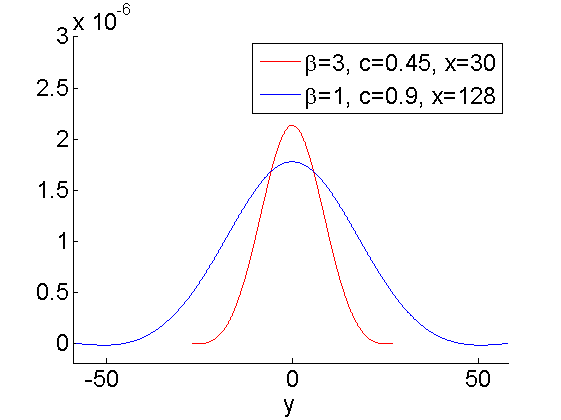
\includegraphics[width=\linewidth]{SolutionView/ChristovIC_128vsChristov_30on_xEnd.png}
	\end{minipage}	
	\begin{minipage}[b]{0.5\linewidth}
		\raggedright
		 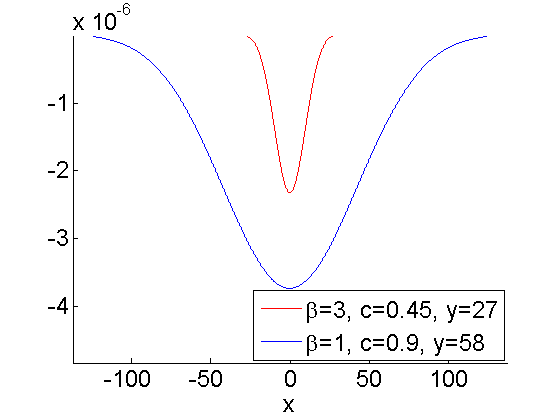
\includegraphics[width=\linewidth]{SolutionView/ChristovIC_128vsChristov_30on_yEnd.png}
	\end{minipage}
	\caption{Сечения на численото решение при Тест 1 ($\beta=3, c=0.45$) и Тест 2 ($\beta=1, c=0.90$) в края на областта $\partial \Omega_h$:  $x=30$ за Тест 1 и $x=128$ за Тест 2 (левия панел);  $y=27$ за Тест 1 и $y=58$ за Тест 2 (десния панел).}
	\label{profilesOnBnd}
\end{figure}
\FloatBarrier
\fi
\begin{figure}[ht]
	\begin{minipage}[b]{0.5\linewidth}
		\raggedleft
		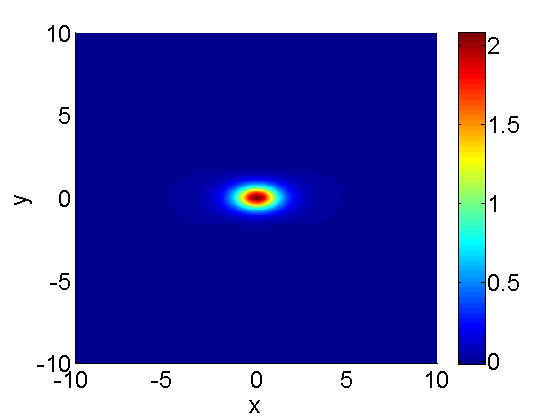
\includegraphics[width=\linewidth]{SolutionView/ChristovIC_30_bt3_c045_topview.png}
	\end{minipage}
	\begin{minipage}[b]{0.5\linewidth}
		\raggedright
		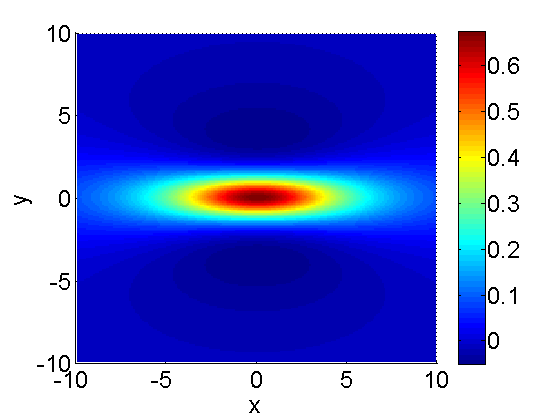
\includegraphics[width=\linewidth]{SolutionView/ChristovIC_128_bt1_c090_topview.png}
	\end{minipage}
	\begin{minipage}[b]{0.5\linewidth}
		 \raggedleft
		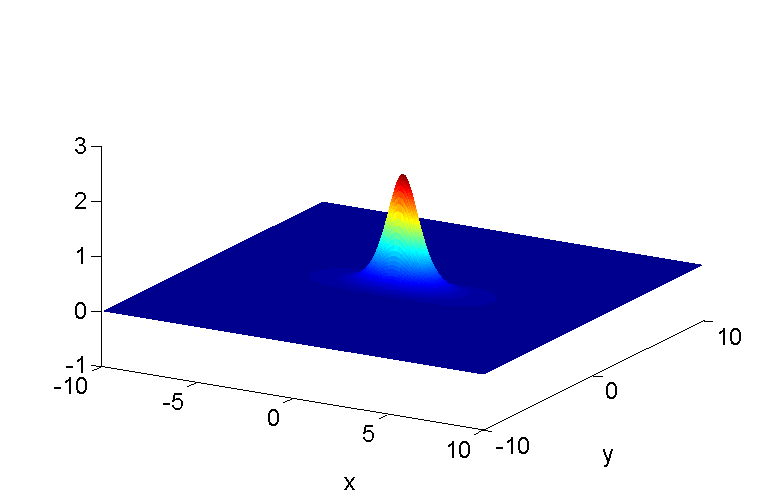
\includegraphics[width=\linewidth]{SolutionView/ChristovIC_30_bt3_c045_prpview.png}		
		\centerline{$\beta = 3$, $c = 0.45$ }
	\end{minipage}
	\begin{minipage}[b]{0.5\linewidth}
		 \raggedright
		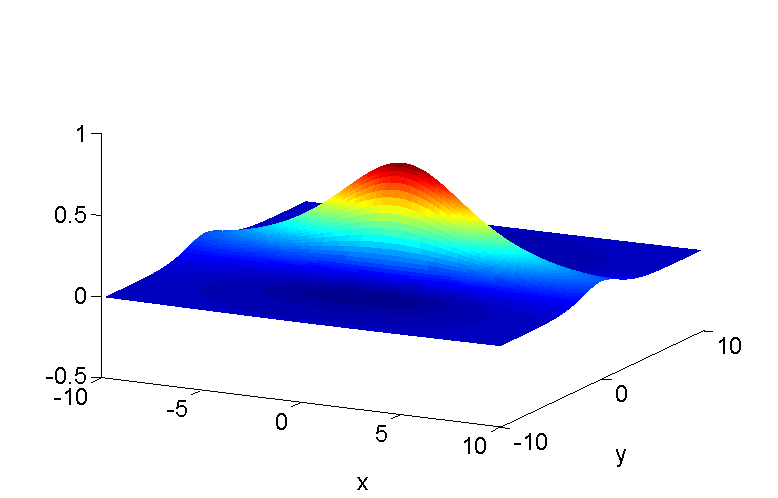
\includegraphics[width=\linewidth]{SolutionView/ChristovIC_128_bt1_c090_prpview.png}
		\centerline{$\beta = 1$, $c = 0.9$}
	\end{minipage}
	\caption{2Д и 3Д профили на численото решение $\widehat v$ от \rf{eqtheta} и \rf{eq555}. За изображенията са избрани най-ситните стъпки - $h=0.05$ (ляво), $h=0.1$ (дясно).}
	\label{fig:solutions}
\end{figure}
\FloatBarrier
\subsection{Числени резултати от метода на простата итерация за решаването на стационарното уравнение на Бусинеск}\label{resultsElliptic}
В тази част са представени резултатите от приложения числен метод, описан по-горе за елиптичното уравнение \rf{eq3}. Потвърждават се и характерните свойства на получените решения за различни стойности на параметрите $\beta$ и $c$, които са представени първоначално в \cite{ref117,ref116}, като например зависимостта на формата на вълната от скоростта $c$ и дисперсията $\beta$ и асимптотичното поведение $\frac{1}{x^2 + y^2}$ при $\sqrt{x^2 + y^2} \rightarrow \infty$. В допълнение са открити и други релации, например за положителните и отрицателните области на решението.
Също така последното е сравнено с ``best-fit'' апроксимационните формули от \cite{ref15}. Tова сравнение липсва в литературата. Tо се оказва съществен елемент и повратна точка в изследването на хиперболичната задача \rf{eq1}-\rf{eq11}. Тук напомняме на читателя, че ``best-fit'' формулите са използвани за начално условие в итерационния алгоритъм.

\subsubsection{Резидуал}

\begin{figure}[ht]
	\begin{minipage}[b]{0.45\linewidth}
		\raggedleft
		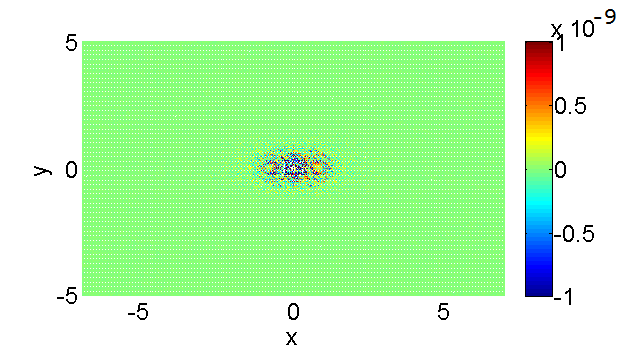
\includegraphics[width=\linewidth]{residual/residual_bt3c045_Oh4.png}
		\centerline{$\beta = 3$, $c = 0.45$}
	\end{minipage}	
	\begin{minipage}[b]{0.45\linewidth}
		\raggedright
		 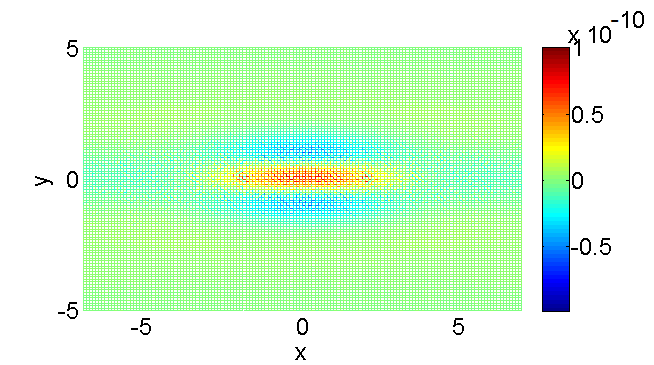
\includegraphics[width=\linewidth]{residual/residual_bt1c090_Oh4.png}
	\centerline{$\beta = 1$, $c = 0.9$ }
	\end{minipage}
	\caption{Резидуала \rf{residual} от решението от последната итерация при уравнения \rf{eq555}, апроксимирано с грешка $O(h^4)$. }
	\label{residOh4}
\end{figure}

\begin{figure}[ht]
	\begin{minipage}[b]{0.45\linewidth}
		\raggedleft
		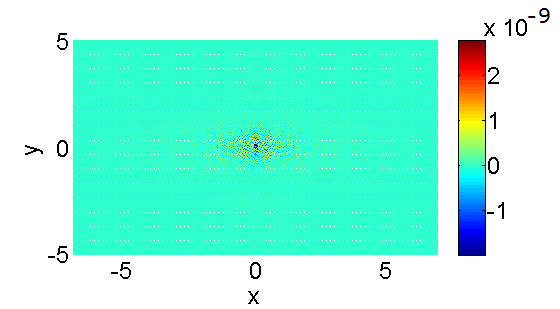
\includegraphics[width=\linewidth]{residual/residual_bt3c045_Oh6.png}
		\centerline{$\beta = 3$, $c = 0.45$}	
	\end{minipage}	
	\begin{minipage}[b]{0.41625\linewidth}	
		 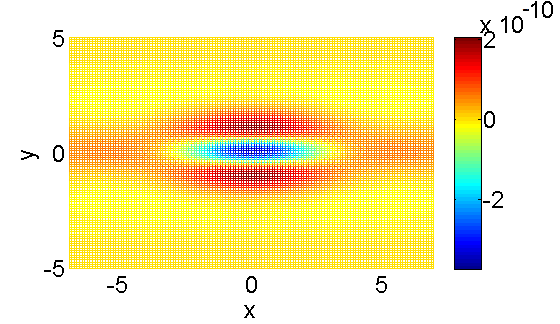
\includegraphics[width=\linewidth]{residual/residual_bt1c090_Oh6.png}
		\centerline{$\beta = 1$, $c = 0.9$ }
	\end{minipage}

	\caption{Резидуала \rf{residual} от решението от последната итерация при уравнения \rf{eq555}, апроксимирано с грешка  $O(h^6)$. }
	\label{residOh6}
\end{figure}
\FloatBarrier
На Фигури \ref{residOh4} и \ref{residOh6} представен резидуалът \rf{residual}, който е запазен от последната стъпка на итерационната схема \rf{eq555}, като за левия панел  параметрите са $\beta = 3$ и $c = 0.45$, а за десния $\beta = 1$ и $c = 0.9$. И в двата случая $\epsilon \le 1e-9$, а използваните крайни разлики представени на фигурите са от четвърти и шести порядък. Резидуалът $R$ на първата итерация е винаги по-голям от $1e-1$ за показаните случаи на Фигури \ref{residOh4} и \ref{residOh6}. 
Разликите в решенията между последните две итерации е $8.7e-13$ и $3.0e-14$ при $O(h^4)$ и $2.3e-16$ и $2.1e-13$ при $O(h^6)$ съответно за първия и втория пример. Така, диференчната схема \rf{eq55} е удовлетворена с голяма прецизност както от апроксимации на вторите производни с до шести ред, така и от ниския праг $\epsilon \le 1\times10^{-9}$. 

От друга страна разглеждайки формулите от ``best-fit'' апроксимацията от \cite{ref15} се вижда, че третите, четвъртите и други производни по пространството от по висок ред са неограничени в околност на нулата $(0,0)$. Така нито елиптичното уравнение \rf{eq3}, нито резидуалът \rf{residual} могат да бъдат пресметнати в класическия смисъл и следователно не са удовлетворени от ``best-fit'' формулите!

\subsubsection{Производни на решението}
\begin{center}
\begin{table}[ht]
\centering
		\begin{tabular}{||c|l|ll|ll||}
			\hline
			\hline
      FDS       & $h$ &errors in $L_2$&Conv. Rate& errors in $L_\infty$&Conv. Rate\\
   			\hline 
					\hline 
      c=0.45    	& 0.2  	&             		&             &                    &   \\
   $O(h^2)$     	& 0.1    	& 0.100892  	&             	& 0.226160 &   \\
                		& 0.05   & 0.022355  	& 2.17  		& 0.052240 &2.11 \\
               	 \hline 
      c=0.45    	& 0.2  	&             		&             &                    &   \\
   $O(h^6)$     	& 0.1    	& 0.005038  	&             &  0.012462 &   \\
                		& 0.05   & 0.000094  	& 5.75 	  &  0.000323 &5.27 \\
			\hline
			\hline 	
      c=0.9     	& 0.4  	&             		&             &                    &   \\
   $O(h^2)$     	& 0.2    	& 0.001565  	&             	&0.001886 &   \\
                		& 0.1    & 0.000302  	& 2.37  		&0.000405 &2.22 \\
               	 \hline 
      c=0.9     	& 0.4  	&             		&             &                    &   \\
   $O(h^6)$     	& 0.2    	& 0.000089  	&             & 0.000117 &   \\
                		& 0.1    & 0.000003  	& 5.02 	  & 0.000004  &4.77 \\
		   \hline
			\hline 
		\end{tabular}
		\caption{Грешките в $L_2$ и $L_\infty$ норми заедно със сходимостта на четвъртите производни по $x$, пресметнати с $O(h^2)$ и $O(h^6)$ апроксимации.}
\label{tab:fourth-der}
\end{table}
\end{center}
\FloatBarrier
Целта на този параграф е да покаже, че дискретните производни на решението от четвърти ред $v_{\widehat{xxxx}}$ схождат числено, когато стъпката $h$ намалява. За целта е приложено правилото на Рунге \rf{Runge} върху три вложени мрежи с размери $h$, $h/2$, $h/4$, а получените резултати за сходимостта $\xi$ са представени в Таблица \ref{tab:fourth-der}. В заключение се вижда, че дискретните производни $v_{\widehat{xxxx}}$ са ограничени и сходящи. Тестове със смесените производни - $v_{\widehat{xxyy}}$ и само по $y$ - $v_{\widehat{yyyy}}$ не са представени тук, но резултатите от тях са подобни като тези при $v_{\widehat{xxxx}}$.

\subsubsection{Форма на решението}

\begin{figure}[ht]
	\begin{minipage}[b]{0.5\linewidth}
		\raggedleft
		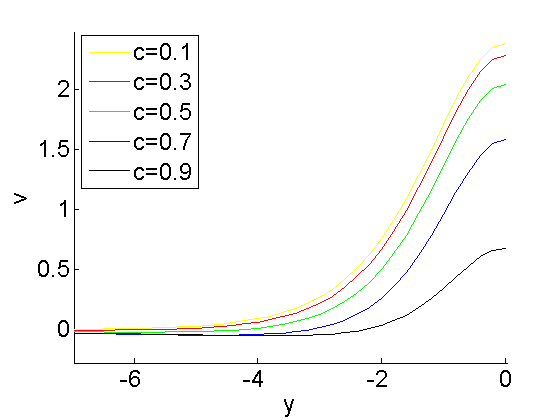
\includegraphics[width=\linewidth]{SolutionProfiles/ChristovIVX=0_ZB2_bt1_c010_090_h020_O(h^6).png}
	\end{minipage}	
	\begin{minipage}[b]{0.5\linewidth}
		\raggedright
		 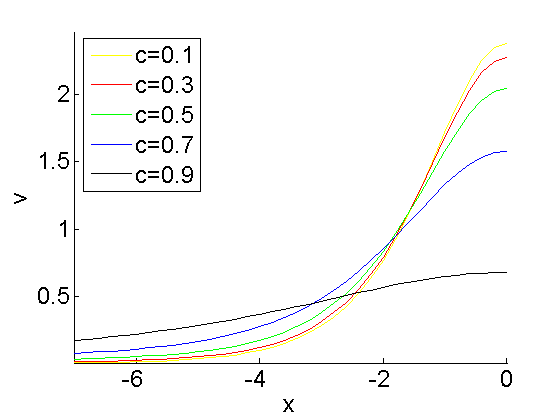
\includegraphics[width=\linewidth]{SolutionProfiles/ChristovIVY=0_ZB2_bt1_c010_090_h020_O(h^6).png}
	\end{minipage}
	\begin{minipage}[b]{0.5\linewidth}
		\raggedleft
		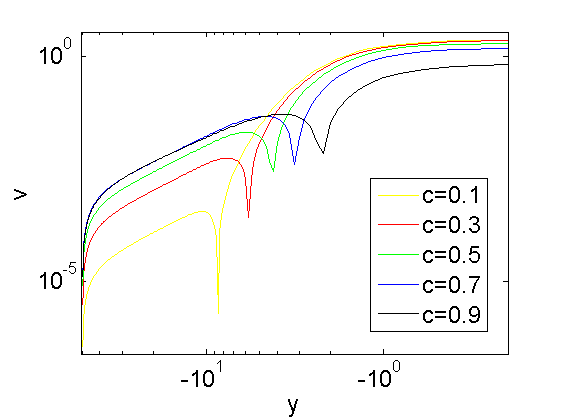
\includegraphics[width=\linewidth]{SolutionProfiles/ChristovIVLogX=0_ZB2_bt1_c010_090_h020_O(h^6).png}
	\end{minipage}	
	\begin{minipage}[b]{0.5\linewidth}
		\raggedright
		 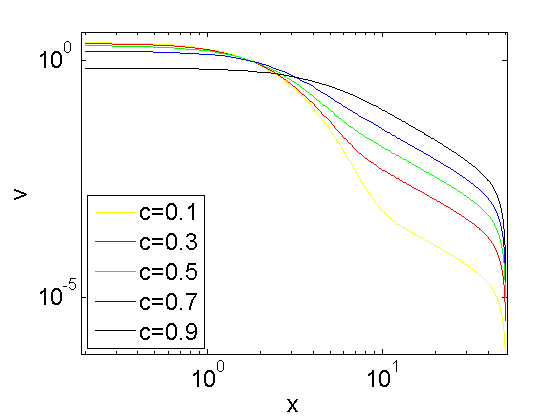
\includegraphics[width=\linewidth]{SolutionProfiles/ChristovIVLogY=0_ZB2_bt1_c010_090_h020_O(h^6).png}
	\end{minipage}
	\caption{Сечения на численото решение по $x$ (ляво) и $y$ (дясно) осите при $\beta=1$ и различни скорости $c=0.1,0.3,0.5,0.7,0.9$. Горните картинки използват реални скали, а долните са изцяло логаритмични.}
	\label{profilesSpeedVarying}
\end{figure}
Фигура \ref{fig:solutions} показва формата на решението получено с параметрите заложени съответно в Тест 1 (ляво $c=0.45$,  $\beta=3$) и Тест 2 (дясно $c=0.9$,  $\beta=1$) при $\alpha = 1$. Показаната област за разгледаните случаи е $[-10,10] \times [-10,10]$. Разбира се, решението е пресметнато в правоъгълника $\omega_h$ и използвайки симетрията му, е построено в цялата област $\Omega_h$, но за да изпъкне формата, която е близо до максимума, стойностите, които са по ръбовете и близки до нула, са изрязани. Вижда се, че при $\beta=1$ дисперсията на вълната е по-голяма (по-разтлана в пространството, но по-ниска) спрямо формата получена при $\beta=3$.

Детайлно са разгледани зависимостите на формата на вълната спрямо два от параметрите - дисперсията $\beta=\beta_1 / \beta_2$ и скоростта $c$.
Фигура \ref{profilesSpeedVarying} показва сеченията на решението при $x=0$ и $y=0$, за различни скорости $c=0.1, 0.3, 0.5, 0.7, 0.9$ при $\beta = 1$. Големината на областта е $L_x = L_y = 50$, стъпката по пространството е $h = 0.2$, а прагът на спиране е $\epsilon = 5.0e-10$. Горните две графики представят резултатите в линеен вид, докато долните две представят резултатите в логаритмични скали по $(y,v)$ и $(x,v)$. При логаритмичните панели от Фигура \ref{profilesSpeedVarying} се вижда асимптотичното поведение на решението $1/x^2$ и $1/y^2$ съответно при сеченията $y=0$ и $x=0$ \cite{ref15, ref117, ref116}. Графиките показват, че с увеличаването на скоростта $c$ максимума на вълната намалява (остротата във върха се губи), заема повече обем по $x$ оста и изтънява по оста на движение $y$. Това поведение е аналогично на резултатите в \cite{ref15, ref117, ref116}.
\begin{figure}[ht]
	\begin{minipage}[b]{0.5\linewidth}
		\raggedleft
		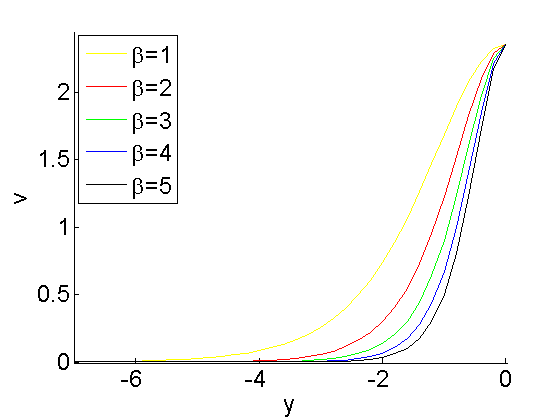
\includegraphics[width=\linewidth]{SolutionProfiles/ChristovIVX=0_ZB2_bt1_5_c017_h020_O(h^6).png}
	\end{minipage}	
	\begin{minipage}[b]{0.5\linewidth}
		\raggedright
		 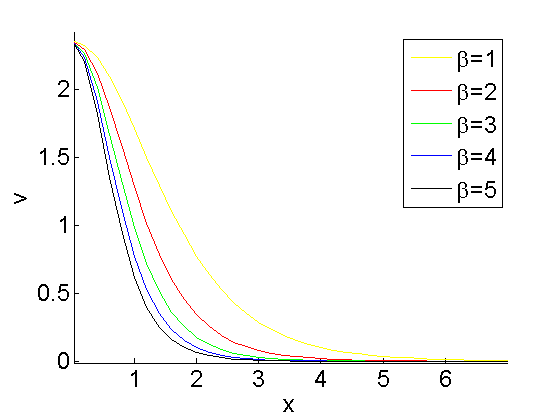
\includegraphics[width=\linewidth]{SolutionProfiles/ChristovIVY=0_ZB2_bt1_5_c017_h020_O(h^6).png}
	\end{minipage}
	\begin{minipage}[b]{0.5\linewidth}
		\raggedleft
		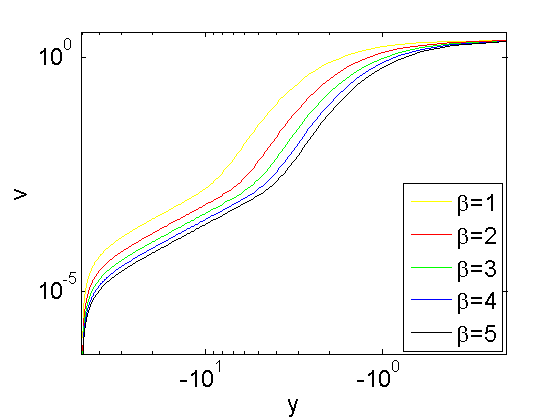
\includegraphics[width=\linewidth]{SolutionProfiles/ChristovIVLogX=0_ZB2_bt1_5_c017_h020_O(h^6).png}
	\end{minipage}	
	\begin{minipage}[b]{0.5\linewidth}
		\raggedright
		 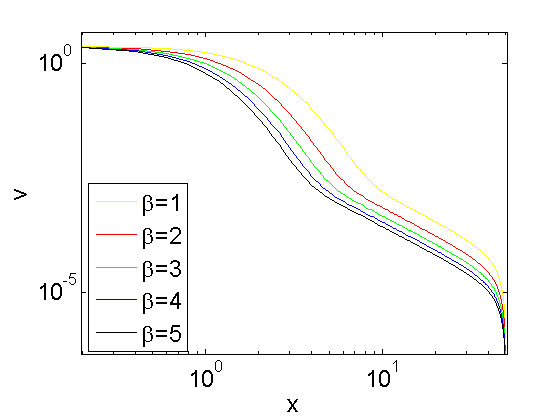
\includegraphics[width=\linewidth]{SolutionProfiles/ChristovIVLogY=0_ZB2_bt1_5_c017_h020_O(h^6).png}
	\end{minipage}
	\caption{Сечения на численото решение по $x$ (ляво) и $y$ (дясно) осите при $c=0.17$ и варираща дисперсия $\beta=1,2,3,4,5$. Горните изображения използват реални скали, а долните са изцяло логаритмични.}
	\label{profilesDispVarying}
\end{figure}
На Фигура \ref{profilesDispVarying} са показани сеченията на решението при $x=0$ и $y=0$, за различни параметри $\beta=1, 2, 3, 4, 5$ при фиксирана скорост $c=0.17$. Горните две графики представят резултатите в линеен вид, докато долните две представят резултатите в логаритмични скали по $(y,v)$ и $(x,v)$. При логаритмичните панели във Фигура \ref{profilesDispVarying} отново изпъква асимптотичното поведение на решението $1/x^2$ и $1/y^2$ съответно при сеченията $y=0$ и $x=0$, както в \cite{ref15, ref117, ref116}. Графиките показват, че с увеличаването на дисперсионния параметър $\beta$ максимумът на вълната намалява и формата ѝ изтънява по $x$ и $y$ осите (изостря се във върха), подобно на \cite{ref15, ref117, ref116}.
\begin{figure}[htbp]
	\begin{minipage}[b]{0.48\linewidth}
		\raggedleft
		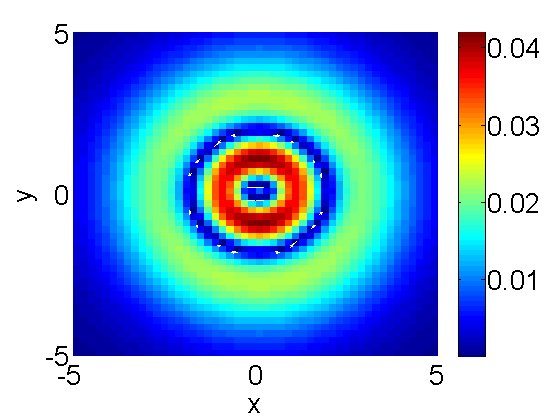
\includegraphics[width=\linewidth]{BestFitVsSimpleIter/ChristovIC_50_bt1_c017_h02_O(h^6).png}
	\end{minipage}
	\begin{minipage}[b]{0.48\linewidth}
		 \raggedright
		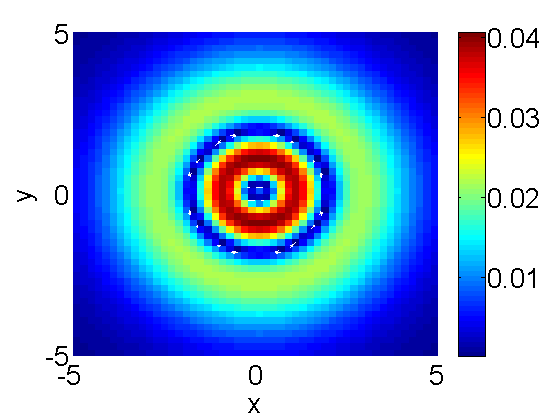
\includegraphics[width=\linewidth]{BestFitVsSimpleIter/ChristovIC_50_bt1_c010_h02_O(h^6).png}
	\end{minipage}
	\begin{minipage}[b]{0.48\linewidth}
		\raggedleft
		 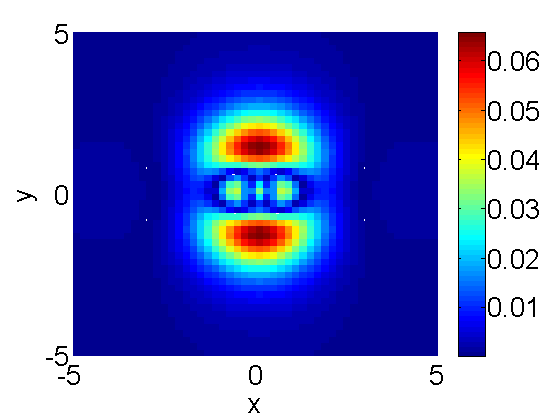
\includegraphics[width=\linewidth]{BestFitVsSimpleIter/ChristovIC_50_bt3_c017_h02_O(h^6).png}
	\end{minipage}
	\begin{minipage}[b]{0.48\linewidth}
		\raggedright
		 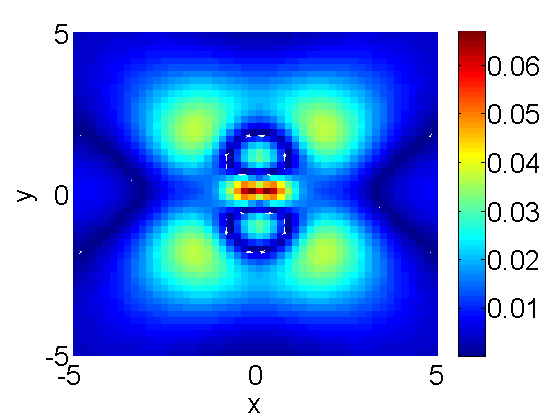
\includegraphics[width=\linewidth]{BestFitVsSimpleIter/ChristovIC_50_bt1_c050_h02_O(h^6).png}
	\end{minipage}
	\begin{minipage}[b]{0.48\linewidth}
		\raggedleft
		 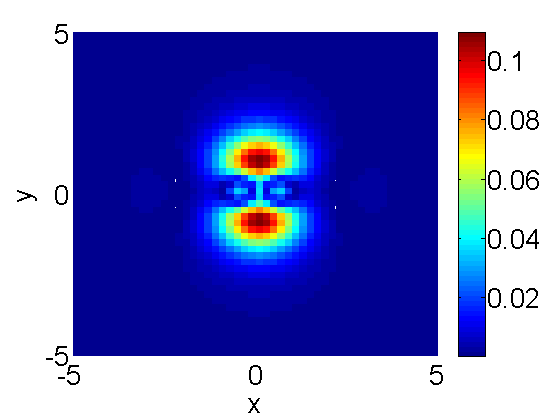
\includegraphics[width=\linewidth]{BestFitVsSimpleIter/ChristovIC_50_bt5_c017_h02_O(h^6).png}
		\centerline{$c=0.17$}
		\centerline{$\beta = 1,3,5$ (от горе надолу) }
	\end{minipage}
	\begin{minipage}[b]{0.48\linewidth}
		\raggedright
		 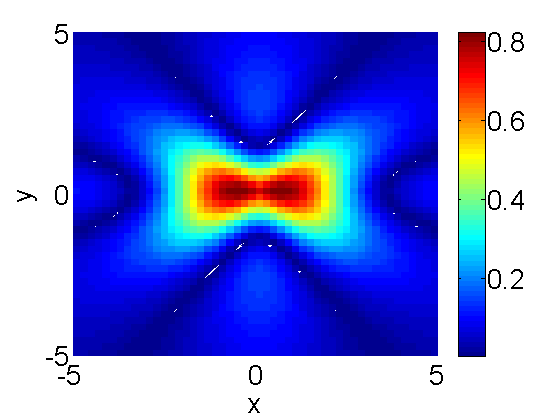
\includegraphics[width=\linewidth]{BestFitVsSimpleIter/ChristovIC_50_bt1_c090_h02_O(h^6).png}
		\centerline{$\beta = 1$}
		\centerline{$c = 0.1, 0.5, 0.9$ (от горе надолу)}
	\end{minipage}
	\caption{Разликите между числено решение $v$ на елиптичната задача при $O(h^6)$ апроксимация и ``best-fit'' формулите $v^*$ от \cite{ref15}. }
	\label{fig:difference}
\end{figure}

\subsubsection{Сравнение с ``best-fit'' формулите от \cite{ref15} }
Фигура \ref{fig:difference} заедно с Таблици \ref{tab:diff-beta1}, \ref{tab:diff-c017} показват разликите в абсолютна стойност между числено решение, получено на последната итерация $v$ от процедурата \rf{eq555} и ``best-fit'' формулите $v^*$. Големината на областта при тези тестове е $L_x = L_y = 50$. При дискретизацията са използвани крайни разлики с шести ред на апроксимация $p=6$, стъпката по пространството е $h=0.2$, а граничното условие е описано в ``Симетрично гранично условие по абцисата и ордината при елиптичната задача''. При Таблица \ref{tab:diff-beta1}, дисперсионния параметър $\beta=1$ е фиксиран, а скоростта $c = 0.1, 0.3, 0.5, 0.7, 0.9$ нараства. При Таблица \ref{tab:diff-c017}, скоростта $c = 0.17$ е фиксирана, а $\beta=1, 2, 3, 4, 5$ нараства. Аналогично е разпределението при графиките от Фигура \ref{fig:difference}, които показват абсолютната разлика между двете функции само в подобласт на $\Omega_h$ - $[-5,  5] \times [-5,5]$, където е най-голяма. Параметърът $\alpha = 1$ е фиксиран. За да получим съпоставка между двете функции коректно в $\Omega_h$, имайки предвид смяната на променливите направена в уравнение \rf{eq3}, се получава:
\be\label{d123}
v^*\left(\sqrt{\beta_1}x_i,\sqrt{\beta_1}y_j\right)-v(x_i,y_j), \quad (x_i,y_j) \in \Omega_h !
\ee
Резултатите от \rf{d123}, за различни параметри $\beta$ и $c$, са представени на Фигура \ref{fig:difference}. Нека $D^*_{\kappa}$ да дефинира процентната разлика между двете решения $v$ и $v^*$ в ${L_2 }$ и ${L_\infty}$ норми, върху цялата област $\Omega_h$:
\be\label{diffvv}
D^*_{\kappa} := 100 \times \frac{\Vert v^*-v \Vert_{\kappa} }{ \Vert v \Vert_{\kappa} }, \; \kappa=2; \; \kappa=\infty.
\ee
Целта е $D^*_{\kappa}$ да служи като обективен показател, който измерва големината на отклонението $v^*(\sqrt{\beta}x,\sqrt{\beta}y)-v(x,y)$, където с $\kappa$ е означена използваната норма - ${L_2 }$ или ${L_\infty}$.
%================================================================

\begin{table}[ht]
\centering
\begin{tabular}{|l|c|l l|l l|}
\hline
\hline 
$\beta$	& c 	& $\|v^*-v \|_{L_2 }$ & $\|v^*-v \|_{L_\infty }$  	& $D^*_{L_2}$	& $D^*_{L_\infty }$	\\
\hline 
1& 		0.1	&	1.4772e-01 		& 	8.1024e-03 				& 2.7\%			& 1.7\%		\\
\hline 
1& 		0.3 	&	1.4310e-01 		& 	8.7770e-03				& 2.7\%			& 1.9\%		\\
\hline 
1& 		0.5 	&	1.6934e-01 		& 	1.3332e-02				& 3.5\%			& 3.3\%		\\
\hline 
1& 		0.7 	&	5.8673e-01		& 	5.1122e-02				& 14.8\%		& 16.2\%	\\
\hline 
1& 		0.9	&	2.1599e+0 		& 	1.6439e-01				& 93.1\%		& 121.2\%	\\
\hline 
\hline 
\end{tabular}
\caption{Разлики между числено решение $v$ на елиптичната задача с висок ред на апроксимация $O(h^6)$ и ``best-fit'' формулите $v^*$ от \cite{ref15} при $\beta=1$ и $c=0.1, 0.3, 0.5, 0.7, 0.9$.}
\label{tab:diff-beta1}
\end{table}
От Таблица \ref{tab:diff-beta1} се вижда, че разликата между двете дискретни функции в $L_2$ норма се увеличава от $2.7\%$ до $93.1\%$, а при $L_\infty$ норма - от $1.7\%$ до $121.2\%$, когато параметърът $c$ расте. Формулата $v^*$ представлява числено решение, което използва развитие в ред около скоростта $c$. Затова при по-големи скорости процентът $D^*_{\kappa}$ нараства рязко, както е описано в \cite{ref15}.

%================================================================

\begin{table}[ht]
\centering
\begin{tabular}{|l|c|l l| c|l|c|l l|}
\hline 
\hline 
$\beta$	& c 	& $\|v^*-v \|_{L_2 }$ & $\|v^*-v \|_{L_\infty }$  	& $D^*_{L_2}$	& $D^*_{L_\infty }$	\\
\hline 
1& 		0.17&	1.4704e-01 		& 	8.3793e-03 				& 2.7\%			& 1.8\%		\\
\hline 
2& 		0.17&	1.2688e-01 		& 	9.0013e-03				& 3.3\%			& 1.9\%		\\
\hline 
3& 		0.17&	1.3803e-01 		& 	1.3134e-02				& 4.4\%			& 2.8\%		\\
\hline 
4& 		0.17&	 1.5240e-01 		& 	1.7228e-02				& 5.7\%			& 3.7\%		\\
\hline 
5& 		0.17&	1.6720e-01 		& 	2.1844e-02				& 7.0\%			& 4.6\%		\\
\hline 
\hline 
\end{tabular}
\caption{Разлики между числено решение $v$ от елиптичната задача с висок ред на апроксимация $O(h^6)$ и ``best-fit'' формулите $v^*$ от \cite{ref15} при $\beta=1, 2, 3, 4, 5$ и $c=0.17$.}
\label{tab:diff-c017}
\end{table}
%================================================================
В Таблица \ref{tab:diff-c017} са получени сходни резултати. При по-големи стойности за $\beta$, процентната разлика нараства до $7.0\%$ и $4.6\%$ съответно в $L_2$ и $L_\infty$ норми. Въпреки всичко, както се вижда от таблиците, с намаляването на скоростта "best-fit" формулите доближават решението от елиптичната задача, получено с висок ред на апроксимация по $L_2$ и $L_\infty$ норми.

В Част \ref{numTestbt3c03} ``Числен тест за хиперболичната задача при параметри $c=0.3$ и $\beta = 3$'' разглеждаме един пример, изследван многократно в  различни научни трудове (виж \cite{ref21, ref20, ref23, ref22}), при който вълната се разсейва на по-малки вълни в пръстеновидна форма. Показано е, че формата и максимума на вълната се запазват за по-дълго време, ако за начално условие в хиперболичната задача, се използва директно решението от елиптичната задача с апроксимация $O(h^4)$ или $O(h^6)$. 

\subsection{Ново гранично условие за двумерното елиптично уравнение \rf{eq3}}\label{newBndHead}
Трябва да се отбележи, че както елиптичното, така и хиперболичното уравнения са дефинирани в цялата равнина $\RR^2$. За да се решат тези уравнения числено се въвежда краен правоъгълник, върху който се построява мрежа $\Omega_h$. Така могат да се получат резултати, които апроксимират непрекъснатото решение в неограничената област, като целият процес трябва да приключи за разумно време (не повече от два-три дни при най-ситните стъпки $h$ и $\tau$). В случай, че за уравнение \rf{eq3} се приложи гранично условие по краищата на областта $\partial \Omega_h$, то със сигурност изчислителната сложност ще намалее, използвайки по-малки области, особено при Тест 2 ($\Omega_h = [-128, 128] \times [-58, 58]$). Гранично Условие (ГУ), което е изведено в тази част, е познато в литературата като абсорбиращо ГУ (виж \cite{ref31} при вълнови уравнения, \cite{ref32} при уравнения от типа на Хелмхолц, \cite{ref33} за елиптични уравнения от втори ред и т.н.). Задачата за намиране на гранично условие е разгледана в \cite{ref116}, където е открита следната асимптотика за търсената функция $v$:
\be
v(x,y) = v(r) ~ \frac{C_v}{r^2}, \quad r>>1
\ee
за достатъчно големи стойности $r = \sqrt{x^2 + y^2}$, където $C_v$ е подходящо подбрана константа. Тази част на дисертацията изследва едно ново асимптотично гранично условие за стационарното ПУБ \rf{eq3}:
\be\label{bndK}
\tilde v(x,y) = \mu_v \frac{ (1-c^2)x^2 - y^2}{ ((1-c^2)x^2 + y^2)^2}, \quad x^2 + y^2 >> 1.
\ee
Получаването на последната формула е процес, при който първоначално са разгледани отделните членове в уравнение \rf{eq3} и тяхната асимптотика далеч от максимума на решението в нулата. В последствие, на базата на извършения числен анализ, е направено допускане за водещите членове в уравнението, които са отговорни за асимптотиката на решението на безкрайност. Така елиптичното уравнение \rf{eq3} се опростява до уравнение на Лаплас с помощта на няколко смени на променливите, както е показано в \cite{bnd}. За последното е изведено аналитичното решение \rf{bndK}, което зависи единствено от координатите $(x,y)$, скоростта $c$ и произволен параметър $\mu_v$. В заключение, посредством серия от числени експерименти, е показана валидността на функцията \rf{bndK} за много големи стойности на радиуса $r$. 

Уравнение \rf{eq3} е еквивалентно на 
\begin{align}\label{eq3full}
&\beta v_{xx} + \beta (1-c^2) v_{yy} - v_{xxxx} - (2-\beta c^2)v_{xxyy} - (1-\beta c^2)v_{yyyy} \nonumber \\ 
&- \alpha \beta (v^2)_{xx} - \alpha \beta (v^2)_{yy}  =0.
\end{align}

Асимптотиката на отделните членове в \rf{eq3full} е описана в серия от експерименти и може да се види на Фигури \ref{fig:assympt_c017bt1}, \ref{fig:assympt_c017bt3} и \ref{fig:assympt_c017bt5}, където $c=0.17$ е фиксирано, а $\beta = 1, 3, 5$ се мени, и Фигури \ref{fig:assympt_beta1c01}, \ref{fig:assympt_beta1c05} и \ref{fig:assympt_beta1c09}, където $\beta=1$ е фиксирано, а $c = 0.1, 0.5, 0.9$ се мени. Съответните числени тестове, показани на картинките, са направени при големина на областта $\Omega_h = [-50, 50] \times [-50, 50]$, с диференчни схеми от шести ред апроксимация $p=6$, стъпка по пространството $h=0.2$, $\alpha = 1$ и праг на спиране $\epsilon \le 5 \times 10^{-10}$. Използвано е гранично условие, описано в секция \ref{symBndHead} ``Симетрично гранично условие по абцисата и ординатата при елиптичната задача'' заедно с метода на простата итерация. Представените графики са в логаритмични скали по $x,y$. На всяка страница долната легенда е обща и за двете картинки с цел по-добро представяне на резултатите. Константите $\gamma_1$, $\gamma_2$ и $\gamma_3$ са коефициентите пред съответните членове от уравнението както следва
\begin{align*}
\gamma_1 = \beta (1-c^2) \\
\gamma_2 = (1-\beta c^2) \\
\gamma_3 = (2-\beta c^2).
\end{align*}
Останалите константи $\gamma_4$, $\gamma_5$, $\gamma_6$ и $\gamma_6$ са подходящо избрани за всяка двойка графики, така че функциите $(r^{-4}, |v_{xx}|)$ и $(r^{-6}, |- (2-\beta c^2)v_{xxyy}|)$ да са равни в началото (при $r=x=20$ на горния панел и при $r=y=20$ на долния панел).

Основният извод е, че водещите членове с най-голяма абсолютна стойност са $\beta v_{xx}$ и $\beta (1-c^2) v_{yy}$, а останалите са по-малки по стойност и порядък. Остатъкът $R$ от \rf{residual}, който също е представен на графиката, е сума от всички членове в уравнението \rf{eq3full} и той е най-малък по абсолютна стойност, т.е. уравнението е удовлетворено числено в разгледаните интервали. 
Изобразявайки функцията $\Psi : \RR \rightarrow \RR$, с уточнението че $\Psi(r) = r^{-n}, n \in \mathbb{N}$, в логаритмични скали представлява граф от вида $(\rho, -n \rho )$, където $\rho := log_{10}(r)$ и $ -n \rho = log_{10}( \Psi(r) ) $, т.е. това е линейна функция с наклон $-n$. Същото свойство е видно и на всички графики от Фигурите \ref{fig:assympt_c017bt1} - \ref{fig:assympt_beta1c09}. Посредством помощните функции $\gamma_4 y^{-4}$, $\gamma_6 x^{-4}$, $\gamma_5 y^{-6}$ и $\gamma_7 x^{-6}$ се открояват различните наклони при членовете 
$$
\beta v_{xx}, \; \beta (1-c^2) v_{yy}
$$ 
с асимптотика $O(r^{-4})$ и 
$$
- v_{xxxx}, \;  - (2-\beta c^2)v_{xxyy},  \;  - (1-\beta c^2)v_{yyyy}, \;  - \alpha \beta (v^2)_{xx}, \; - \alpha \beta (v^2)_{yy}
$$
с асимптотика $O(r^{-6})$, които са съответно $-4$ в първия и $-6$ във втория случаи.
\begin{figure}[ht]
	\begin{minipage}[b]{0.95\linewidth}
		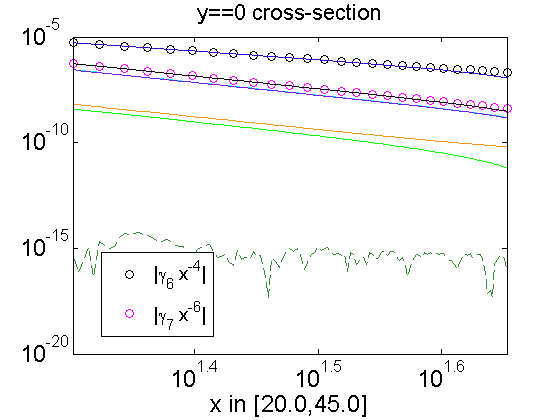
\includegraphics[width=\linewidth]{AssymptForEachTerm/c017_bt1_5/ChristovIC_AlongX_50_ZB2_bt1_c017_h020_O(h^6).png}
	\end{minipage}
	\begin{minipage}[b]{0.95\linewidth}
		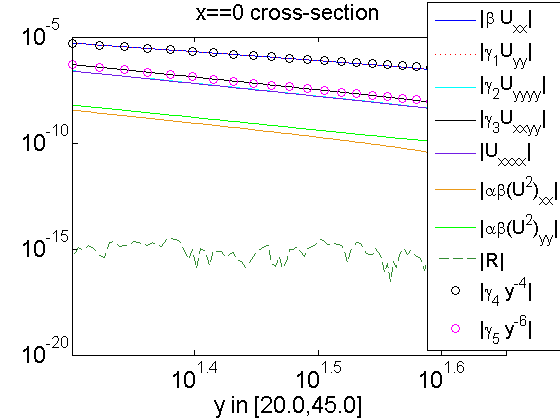
\includegraphics[width=\linewidth]{AssymptForEachTerm/c017_bt1_5/ChristovIC_AlongY_50_ZB2_bt1_c017_h020_O(h^6).png}
	\end{minipage}
	\caption{Асимптотично поведение на членовете от елиптичното уравнение \rf{eq3full}, представени в абсолютна стойност и логаритмични скали по $x,y$, получено с апроксимация от шести ред и нулево гранично условие. Скоростта и дисперсионният параметър са $\boldsymbol{c=0.17}$ и $\boldsymbol{\beta = 1}$. }
	\label{fig:assympt_c017bt1}
\end{figure}
\FloatBarrier
\begin{figure}[ht]
	\begin{minipage}[b]{0.95\linewidth}
		\raggedleft
		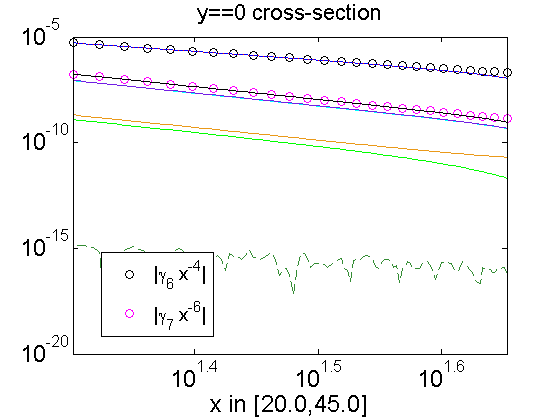
\includegraphics[width=\linewidth]{AssymptForEachTerm/c017_bt1_5/ChristovIC_AlongX_50_ZB2_bt3_c017_h020_O(h^6).png}
	\end{minipage}
	\begin{minipage}[b]{0.95\linewidth}
		 \raggedright
		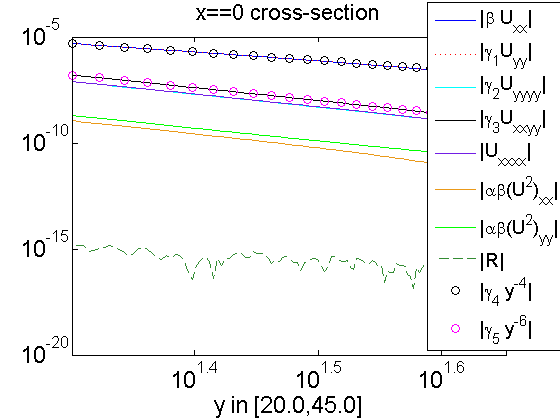
\includegraphics[width=\linewidth]{AssymptForEachTerm/c017_bt1_5/ChristovIC_AlongY_50_ZB2_bt3_c017_h020_O(h^6).png}
	\end{minipage}
	\caption{Асимптотично поведение на членовете от уравнение \rf{eq3full}, представени в абсолютна стойност и логаритмични скали по $x,y$, получено с апроксимация от шести ред и нулево гранично условие. Скоростта и дисперсионният параметър са $\boldsymbol{c=0.17}$ и $\boldsymbol{\beta = 3}$.}
	\label{fig:assympt_c017bt3}
\end{figure}
\FloatBarrier
\begin{figure}[ht]
	\begin{minipage}[b]{0.95\linewidth}
		\raggedleft
		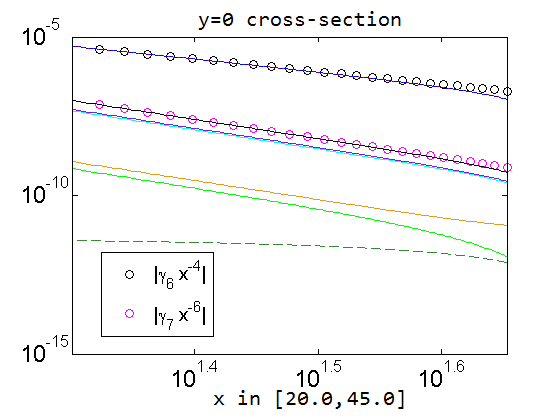
\includegraphics[width=\linewidth]{AssymptForEachTerm/c017_bt1_5/ChristovIC_AlongX_50_ZB2_bt5_c017_h020_O(h^6).png}
	\end{minipage}
	\begin{minipage}[b]{0.95\linewidth}
		 \raggedright
		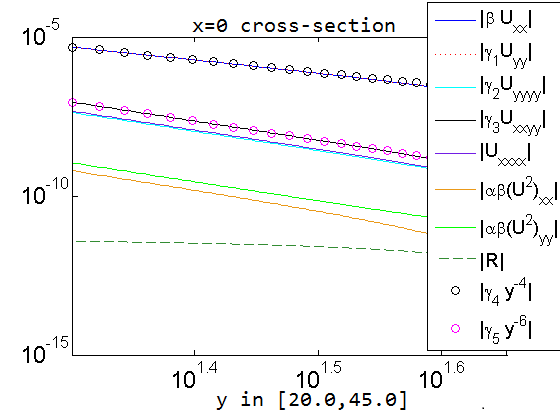
\includegraphics[width=\linewidth]{AssymptForEachTerm/c017_bt1_5/ChristovIC_AlongY_50_ZB2_bt5_c017_h020_O(h^6).png}
	\end{minipage}
	\caption{Асимптотично поведение на членовете от уравнение \rf{eq3full}, представени в абсолютна стойност и логаритмични скали по $x,y$, получено с получено с апроксимация от шести ред и нулево гранично условие. Скоростта и дисперсионният параметър са $\boldsymbol{c=0.17}$ и $\boldsymbol{\beta = 5}$.}
	\label{fig:assympt_c017bt5}
\end{figure}
\FloatBarrier
%end----------------
\begin{figure}[ht]
	\begin{minipage}[b]{0.95\linewidth}
		\raggedleft
		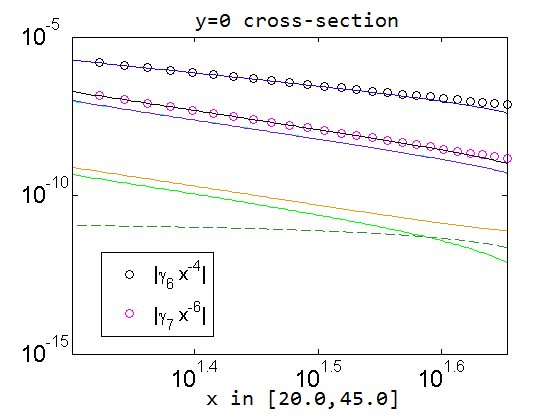
\includegraphics[width=\linewidth]{AssymptForEachTerm/bt1_c010_090/ChristovIC_AlongX_50_ZB2_bt1_c010_h020_O(h^6).png}
	\end{minipage}
	\begin{minipage}[b]{0.95\linewidth}
		 \raggedright
		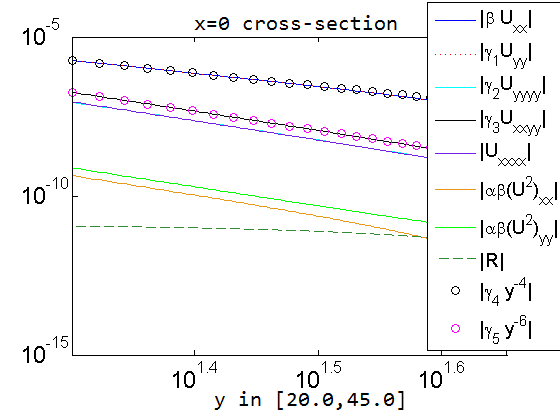
\includegraphics[width=\linewidth]{AssymptForEachTerm/bt1_c010_090/ChristovIC_AlongY_50_ZB2_bt1_c010_h020_O(h^6).png}
	\end{minipage}
	\caption{Асимптотично поведение на членовете от уравнение \rf{eq3full}, представени в абсолютна стойност и логаритмични скали по $x,y$, с получено с апроксимация от шести ред и нулево гранично условие. Скоростта и дисперсионният параметър са $\boldsymbol{c=0.1}$ и $\boldsymbol{\beta = 1}$. }
	\label{fig:assympt_beta1c01}
\end{figure}
\FloatBarrier

\begin{figure}[ht]
	\begin{minipage}[b]{0.95\linewidth}
		\raggedleft
		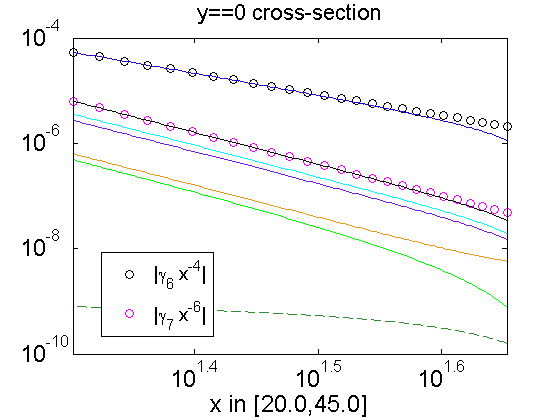
\includegraphics[width=\linewidth]{AssymptForEachTerm/bt1_c010_090/ChristovIC_AlongX_50_ZB2_bt1_c050_h020_O(h^6).png}
	\end{minipage}
	\begin{minipage}[b]{0.95\linewidth}
		 \raggedright
		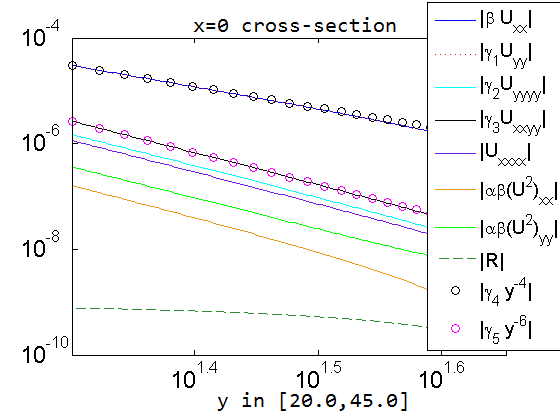
\includegraphics[width=\linewidth]{AssymptForEachTerm/bt1_c010_090/ChristovIC_AlongY_50_ZB2_bt1_c050_h020_O(h^6).png}
	\end{minipage}
	\caption{Асимптотично поведение на членовете от уравнение \rf{eq3full}, представени в абсолютна стойност и логаритмични скали по $x,y$, с получено с апроксимация от шести ред и нулево гранично условие. Скоростта и дисперсионният параметър са $\boldsymbol{c=0.5}$ и $\boldsymbol{\beta = 1}$. }
	\label{fig:assympt_beta1c05}
\end{figure}
\FloatBarrier

\begin{figure}[ht]	
	\begin{minipage}[b]{0.95\linewidth}
		\raggedleft
		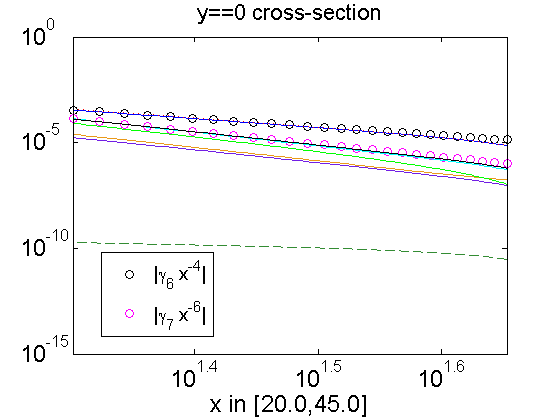
\includegraphics[width=\linewidth]{AssymptForEachTerm/bt1_c010_090/ChristovIC_AlongX_50_ZB2_bt1_c090_h020_O(h^6).png}
	\end{minipage}
	\begin{minipage}[b]{0.95\linewidth}
		 \raggedright
		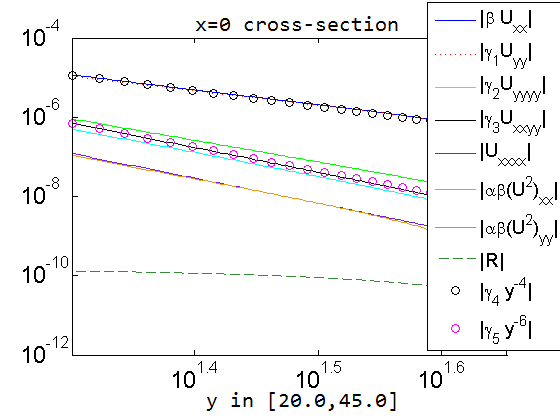
\includegraphics[width=\linewidth]{AssymptForEachTerm/bt1_c010_090/ChristovIC_AlongY_50_ZB2_bt1_c090_h020_O(h^6).png}
	\end{minipage}
	\caption{Асимптотично поведение на членовете от уравнение \rf{eq3full}, представени в абсолютна стойност и логаритмични скали по $x,y$, с получено с апроксимация от шести ред и нулево гранично условие. Скоростта и дисперсионният параметър са $\boldsymbol{c=0.9}$ и $\boldsymbol{\beta = 1}$. }
	\label{fig:assympt_beta1c09}
\end{figure}
\FloatBarrier
\subsubsection{Извoд на новото гранично условие, дефинирано в \rf{bndK} }
Представените фигури в предишната част показват, че асимптотиката на членовете с производни от четвърти ред и нелинейните такива с производни от втори ред в \rf{eq3full}
\be\label{outliers}
- v_{xxxx}, \;  - (2-\beta c^2)v_{xxyy},  \;  - (1-\beta c^2)v_{yyyy}, \;  - \alpha \beta (v^2)_{xx}, \; - \alpha \beta (v^2)_{yy}
\ee
e $O(r^{-6})$, а за останалите от втори ред
$$
\beta v_{xx}, \; \beta (1-c^2) v_{yy}
$$
асимптотиката е $O(r^{-4})$. Това дава основание да пренебрегнем членовете описани в \rf{outliers} от уравнение \rf{eq3full} и да търсим точно решение на останалата част. Така за големи стойности на $r$, пренебрегвайки частите с по-нисък порядък $O(r^{-6})$, остават два водещи члена:
\be\label{asymptEq}
\beta \tilde v_{xx} + \beta (1-c^2) \tilde v_{yy} =0, \quad \tilde v(x,y) \approx \frac{1}{x^2 + y^2}, \quad x^2 + y^2 >>1,
\ee
взимайки предвид факта, че функцията $v(r)$ има асимптотика $O(r^{-2})$.

Следната смяна $\bar x  = \sqrt{1-c^2} x$, $\bar y = y$ и $\tilde V (\bar x, \bar y)$ на променливите трансформира \rf{asymptEq} в уравнението на Лаплас:
\be\label{LaplaceEq}
\Delta \tilde V(\bar x, \bar y) = 0, \quad \tilde V(\bar x, \bar y) = \frac{1}{\bar r^2}, \quad \bar r = \sqrt{\bar x^2 + \bar y^2} \rightarrow \infty.
\ee
Последното в полярни координати има следния вид:
\begin{align}\label{LaplacePolar}
&\frac{\partial^2}{\partial \bar r^2} \tilde V_p(\bar r,\bar \phi) + \frac{1}{\bar r} \frac{\partial}{\partial \bar r} \tilde V_p(\bar r, \bar \phi) + \frac{1}{\bar r^2} \frac{\partial^2}{\partial \bar \phi^2} \tilde V_p(\bar r, \bar \phi) = 0 \\
&\bar \phi = arctan(\frac{\bar y}{\bar x}) \nonumber
\end{align}
%$\tilde V_p(\bar r, \bar \phi) = H(\bar r) G(\bar \phi)$
След прилагане на метода за разделяне на променливите в \rf{LaplacePolar} за решението му се получават следните функции:
\begin{align}\label{LaplaceSol}
&\tilde V_p(\bar r, \bar \phi) = \sum^{\infty}_{n=0} H_n(\bar r) G_n(\bar \phi) =
\\ \nonumber &\sum^{\infty}_{n=0} (\mu_{1,n} \frac{1}{ \bar{r}^n} + \mu_{2,n} \bar{r}^n ) (\mu_{3,n} \sin(n \bar \phi ) + \mu_{4,n}\cos(n \bar \phi)),
\end{align}
където $\mu_{1,n}, \mu_{2,n}, \mu_{3,n}, \mu_{4,n}, n \in \mathbb{N}_{0}$ са реални константи. Скобите с първия множител се опростяват до вида
\be
H_2(\bar r) = \mu_{1,2}\frac{1}{\bar r^2}, \quad \mu_{1,n} = 0, n \neq 2, \quad \mu_{2,n} = 0, n \ge 0
\ee
знаейки, че решението има асимптотика от вида $1/r^2$. За втория множител се получава
\be
G_2(\bar \phi) = \mu_{4,2}\cos(2 \bar \phi), \quad \mu_{3,n} = 0, n \ge 0, \quad \mu_{4,n} = 0, n \neq 2.
\ee
знаейки, че численото решение за достатъчно големи $r >> 1$ е положително върху абцисата и отрицателно върху ординатата (по посока на движение на вълната). Последното е известно от всички направени до момента числени експерименти, независимо от типа на използваното гранично условие. Крайната формула за решението на \rf{LaplacePolar} е:
\be \label{LaplaceSol2}
\tilde V_p(\bar r, \bar \phi) = \mu_v \frac{ \cos(2 \bar \phi) }{ \bar r^2 } = \mu_v \frac{ \cos(\bar \phi)^2 - \sin(\bar \phi)^2 }{ \bar r^2 } = \mu_v \frac{ \bar x^2 - \bar y^2 }{ (\bar x^2 + \bar y^2)^2 },
\ee
където $\mu_v = \mu_{1,2} \mu_{4,2}$. В старите $(x, y, r=\sqrt{x^2+y^2})$ координати \rf{LaplaceSol2} е еквивалентно на 
\be\label{bndv}
\tilde v(x, y) = \mu_v \frac{ (1-c^2) x^2 - y^2 }{ ((1-c^2) x^2 + y^2)^2 }.
\ee
Параметърът $\mu_v$ се намира числено чрез минимизиране на функционала
\begin{equation}\label{eqMin}
\mu_v = \min_{ \mu_v > 0 } || \tilde v( x_i, y_j) - \widehat v^{(k)}_{i,j} ||_{L_2}, \quad (x_i, y_j) \in \omega_B ,
\end{equation}
където $\omega_B$ е областта до външната граница
\be\label{omegaB}
\omega_B = \{ (x_i, y_j) \in \omega_h \: | \: x_i > \frac{7L_x}{8} \; \textbf{или} \; y_j > \frac{7L_y}{8} \},
\ee
а с $\widehat v^{(k)}$ е означено решението получено при $k$-тата итерация от процедурата \rf{eq55}. Минимизационната задача, дефинирана в \rf{eqMin}, е еквивалента на решаването на линейно уравнение спрямо $\mu_v$. Централните крайни разлики, използвани при апроксимацията на оператора на Лаплас и описани в Таблица \ref{table:A00}, не се променят по границата $x=L_x$ и $y=L_y$. За целта при $p=2$ областта $\omega_h$ се разширява по $x$ и по $y$ с една стъпка $h$, при $p=4$ с две стъпки $2h$ и при $p=6$ с три стъпки $3h$.
Стойностите на $\widehat v$ във възлите от увеличената област, които са извън $\omega_h$, се изчисляват използвайки граничната функция $\tilde v(x, y)$.

\subsubsection{Числени резултати за елиптичната задача, получени с новото гранично условие и апроксимация от четвърти ред}
Два числени теста са направени за валидация на формула \rf{bndv}. Първият експеримент разглежда поведението на решението по границата, когато размерите на дискретната област $\Omega_h$ нарастват - $L_x = L_y = 20, 40, 80, 160$. Численото решение $\widehat v$ е сравнено първо, с аналитичния израз от \rf{bndv} върху граничния участък $\omega_B$ (дефиниран в \rf{omegaB}) и второ с численото решение, получено със същите дискретни стъпки, ред на апроксимация и параметри $\alpha, \beta, c$, но при нулево гранично условие дефинирано в Част \ref{symBndHead}. 

Вторият тест разглежда поведението на функцията $\widehat v$ и нейната асимптотика по $x,y$ осите. Отделено е и внимание на това къде в двумерната област $\Omega_h$ численото решение е с положителен знак и къде с отрицателен.

\subsubsection{Експеримент 1 за  гранично условие \rf{bndv}}
В тази част е показано решението на елиптичната задача с новото гранично условие, като са използвани диференчни схеми с четвърти ред на апроксимация $p=4$ и параметрите в \rf{eq55} са дефинирани както следва: $\alpha = 1$, $\beta = 3$ и $c=0.45$. Разгледани са четири различни по големина области $\omega_h = [0, L_x] \times [0, L_y]$, където $L_x = L_y = 20, 40, 80, 160$ и фиксирана стъпка по пространството $h=0.5$. В Таблица \ref{tab:valBnd1} са представени резултати, получени в края на итерационната процедура \rf{eq55} и прилагайки ГУ от \rf{bndv}. Първата колона описва размера на областта. Във втората колона е показана стойността на функцията $\widehat{v}_{i,j}$ в точката: ${x}_i = 0$, $ {y}_j =   L_{ y}$. Поведението на параметъра $\mu_v$ е представено в третата колона. Най-накрая се вижда разликата между граничната функция \rf{bndv} и численото решение $\widehat{v}$ от последната итерация върху $\omega_B$ (виж \rf{omegaB}) в $L_2$ норма.
\begin{table}[ht]
\centering
		\begin{tabular}{||c||c|c|c||}
			\hline
			\hline
      $ L_{ x} = L_{ y}$        &         $\widehat{v}_{i,j}^k$ в  $({x}_i, {y}_j) = (0, L_{ y})$    &    $\mu_v$  &   \mbox{$min|| \tilde v( x_i, y_j) - \widehat v ^k_{i,j} ||_{L_2,\omega_B}$}\\
   			\hline
			\hline
      20    & -2.23e-04    &  1.9355e-01  &     4.17e-05  \\
               	 \hline
    40      & -5.65e-05   &   1.9369e-01    &    4.42e-06 \\
			\hline 	
      80    & -1.41e-05  &      1.9378e-01      &       7.56e-07  \\
			\hline 	
     160     & -3.53e-06  &    1.9381e-01        &     7.44e-10 \\
		   \hline
	             \hline
                     \end{tabular}
\caption{Свойства на решението и гранично условие при различни големини на областта $\omega_h$.}
\label{tab:valBnd1}
\end{table}
\FloatBarrier

В Таблица \ref{tableBnd} са сравнени резултатите между числените решения с гранично условие \rf{bndv} и нулево гранично условие. Използвани са едни и същи дискретни стъпки, ред на сходимост и параметри $\alpha, \beta, c$, описани в горния параграф. В първата колона е представена големината на областта. Във втората и третата колона са представени разликите съответно в $L_2$ и $L_\infty$ норми. Максимумът на решението е представен в последната колона.
\begin{table}[ht]
\centering
\small
		\begin{tabular}{||c|l|l|l||}
			\hline
			\hline
      $ L_{ x} = L_{ y}$        &  $|| \widehat v_{WithB} - \widehat v_{ZeroB} ||_{L_2,\omega_B}$  & $|| \widehat v_{WithB} - \widehat v_{ZeroB} ||_{L_\infty,\omega_B}$     &   $|| \widehat v_{WithB} ||_{L_\infty,\Omega_h}$ \\
   			\hline
			\hline
      20    & 7.019e-03   &  5.102e-04    	&     2.195508  \\
               	 \hline
    40      & 3.606e-03   &   1.342e-04    &    2.195506 \\
			\hline 	
      80    & 1.829e-03  &      3.444e-05  &  2.195506 \\
			\hline 	
     160     & 9.210e-04  &    8.725e-06 	& 2.195506 \\
	   \hline
		\hline 
		\end{tabular}
		\caption{Разликата $||\widehat v_{WithB} - \widehat v_{ZeroB}||_{\kappa,\omega_B}$ в $L_2$ и $L_\infty$ норми между числените решения $v_{WithB}$ с гранично условие \rf{bndv} и $v_{ZeroB}$ с нулево такова за елиптичната задача \rf{eq45}. Решенията са получени по метода на простата итерация с дискретната стъпка $h=0.5$ и апроксимация на вторите производни от четвърти ред. }
\label{tableBnd}
\end{table}
\FloatBarrier

Резултатите от Таблица \ref{tab:valBnd1} показват, че параметърът $\mu_v$ се установява, понеже разликата между две последователни стойности намалява с увеличаването на областта. В допълнение, функцията $\widehat v(0,L_y)$ намалява с темп от вида $1/r^2$. Разликите между численото решение $\widehat v$ и граничната функция $\tilde v$ в $\omega_B$ намаляват при по-големи размери $L_x, L_y$. 

При сравнението между числените решения $v_{WithB}$ с гранично условие от \rf{bndv} и $v_{ZeroB}$ с нулево такова за елиптичната задача \rf{eq45} се вижда, че $L_2$ нормата от разликата намалява два пъти, а $L_\infty$ нормата четири пъти, при двойно увеличение на областта. 

\subsubsection{Експеримент 2 за гранично условие \rf{bndv}}
В тази част е показано численото решение на елиптичната задача с новото гранично условие и са разгледани различни аспекти от неговата асимптотика. Тук размерът на областта $\omega_h = [0, 50] \times [0, 50]$ е фиксиран. Използвани са диференчни схеми с четвърти ред на апроксимация $p=4$ и параметрите в \rf{eq55} са дефинирани както следва: $\alpha = 1$, $\beta = 3$ и $c=0.45$. Единствено стъпката по пространството се мени $h=0.1, 0.2, 0.4, 0.8$.
\begin{figure}[ht]
	\begin{minipage}[b]{0.5\linewidth}
		\raggedleft
		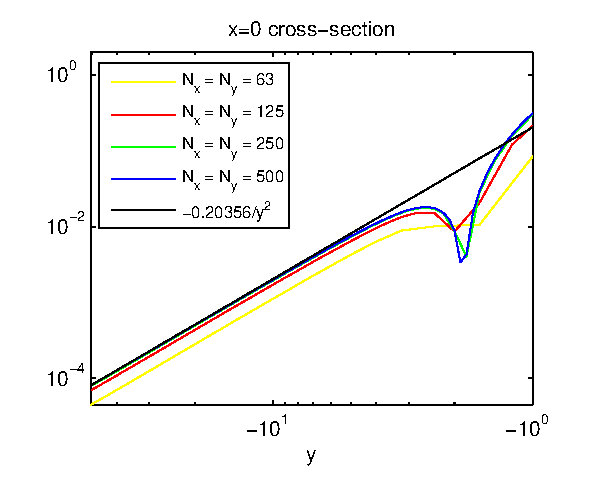
\includegraphics[width=\linewidth]{NewBoundaryCondition/crossSectionLogX=0.eps}
	\end{minipage}	
	\begin{minipage}[b]{0.5\linewidth}
		\raggedright
		 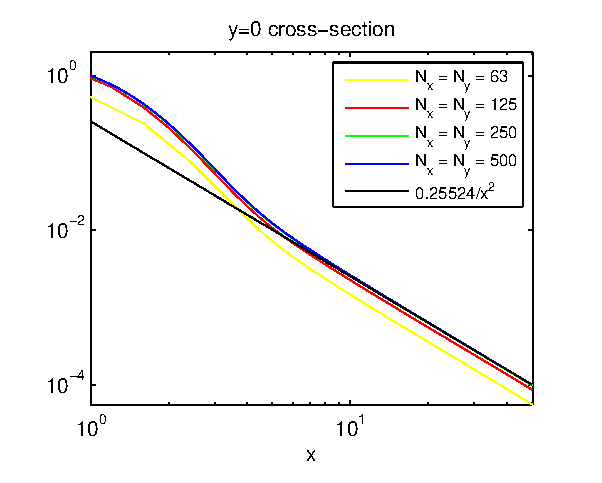
\includegraphics[width=\linewidth]{NewBoundaryCondition/crossSectionLogY=0.eps}
	\end{minipage}
	\begin{minipage}[b]{0.5\linewidth}
		\raggedleft
		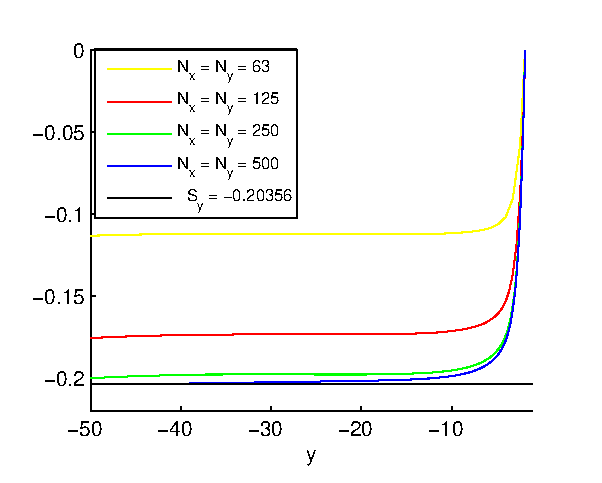
\includegraphics[width=\linewidth]{NewBoundaryCondition/crossSectionX=0FF.eps}
	\end{minipage}	
	\begin{minipage}[b]{0.5\linewidth}
		\raggedright
		 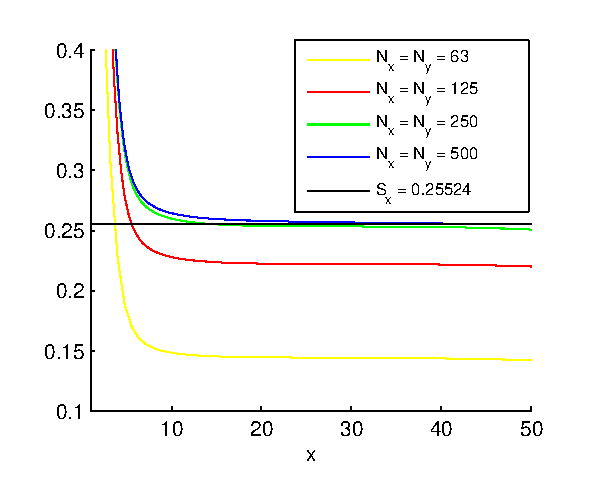
\includegraphics[width=\linewidth]{NewBoundaryCondition/crossSectionY=0FF.eps}
	\end{minipage}
	\caption{Ефектът от промяната на дискретната стъпка по пространството $h=0.1, 0.2, 0.4, 0.8$. На горните панели се вижда функцията $\widehat{v}$ в логаритмични скали по $x,\widehat v(x,0)$ и $y,\widehat v(0,y)$. На долните панели са разположени следните криви: $(y, y^2 \widehat v(0,y)), \; (x, x^2 \widehat v(x,0))$. }
	\label{fig:bndCross}
\end{figure}
\FloatBarrier
Горните две графики от Фигура \ref{fig:bndCross} представят решението в абсолютна стойност върху логаритмични скали по осите $(y,\widehat v(0,y) )$ и $(x,\widehat v(x,0))$. Ясно се вижда, че численото решение за всяка от стъпките $h$ следва наклона на функцията $1/r^2$ за достатъчно големи $r >> 1$. Долните две графики показват численото решение, скалирано с множител $r^2$, т.е. това са кривите $(y, y^2 \widehat v(0, y) )$ и $(x, x^2 \widehat v(y, x) )$. Скалираният профил на решението апроксимира константа: $s_y=-0.20356$ (за левия панел) и $s_x=0.25542$ (за десния панел), за достатъчно големи $r >> 1$. Тези графики са в съответствие с новото ГУ от \rf{bndv} и асимптотиката намерена в \cite{ref116}. В допълнение, използвайки \rf{bndv} за гореописаните случаи при $x=0$ и $y=0$, може да се изведат следните изрази:
\be
\tilde v(0, y) = -\mu_u \frac{1}{y^2}, \quad \tilde v(x, 0) = \frac{\mu_u}{(1-c^2)} \frac{1}{x^2}.
\ee
От последните формули се получават константите $s_x$ и $s_y$ показани в долните панели на Фигура \ref{fig:bndCross}.

\subsubsection{Положителните и отрицателните области на численото решение в $\Omega_h$ }
\begin{figure}[ht]
	\begin{minipage}[b]{0.46\linewidth}
		\raggedleft
		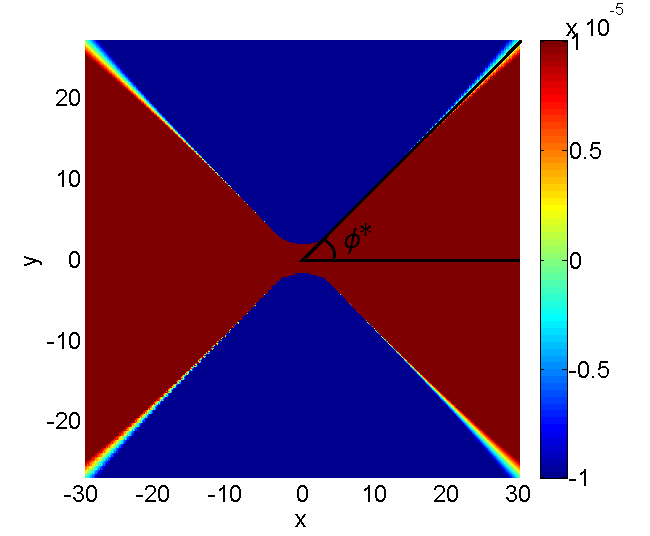
\includegraphics[width=\linewidth]{NewBoundaryCondition/PosNeg_bt3_c045.png}
	\end{minipage}	
	\begin{minipage}[b]{0.49\linewidth}
		\raggedright
		 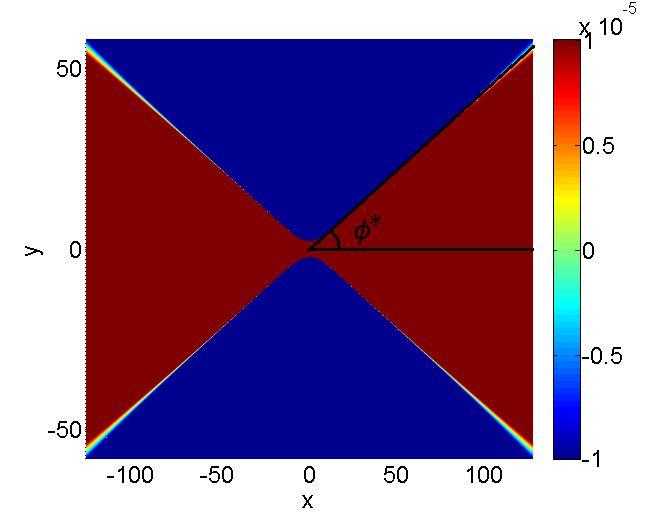
\includegraphics[width=\linewidth]{NewBoundaryCondition/PosNeg_bt1_c090.png}
	\end{minipage}
	\caption{Положителните и отрицателните области на численото решение $\widehat v$ при $\beta = 3, c=0.45$ (левия панел) и $\beta = 1, c=0.90$ (десния панел). }
	\label{fig:posNegDom}
\end{figure}
\FloatBarrier
Фигура \ref{fig:posNegDom} показва знака на численото решение $\widehat v$ получено с граничното условие \rf{bndv} при $\beta=3, c=0.45$ на левия панел и при $\beta=1, c=0.9$ на десния панел. Използвани са диференчни схеми с шести ред на апроксимация $p=6$ и $h=0.1$ при първия тест и $h=0.2$ при втория тест. Цветовият интервал е дефиниран както следва: $[-10^{-5}, 10^{-5}]$. Всяка точка под долната граница на интервала $-10^{-5}$ е оцветена в тъмно синьо, а над горната $10^{-5}$ съответно в тъмно червено. Ясно се забелязват очертанията на три области: южна и северна, които са отрицателни и централна, която е положителна. За достатъчно големи стойности $r >> 1$ се забелязва следната зависимост
\begin{align}\label{posNegFromula}
&\widehat v(r, \phi) > 0 \quad \text{ако} \quad \phi \in (-\phi^*, \phi^*) \cup (\pi - \phi^*, \pi + \phi^*)  \nonumber\\
&\widehat v(r, \phi) < 0 \quad \text{ако} \quad \phi \in (\phi^*, \pi - \phi^*) \cup (\pi + \phi^*, 2\pi-\phi^*) \nonumber\\
&\phi^* = atan(\frac{ \sqrt{1-c^2} }{ 1}).
\end{align}
Свойството \rf{posNegFromula} се използва при определяне на дължините $L_x$ и $L_y$ на числената област $\omega_h$. В зависимост от подбраните стойности $L_x$ и $L_y$ масата на численото решение изчислена върху $\Omega_h$ варира. Примерите в настоящата работа, които се занимават с изследване на масата, са с такива размери на числената област, че да е изпълнено $\frac{L_y}{L_x} \approx \frac{ \sqrt{1-c^2} }{ 1}$. По този начин се получава един баланс между отрицателните и положителните области и независимо от стойностите $L_x, L_y$, стига да е спазено по-горното съотношение, масата не се променя съществено. В допълнение стойностите по северната и южна граници са винаги отрицателни, а по западната и източната -  положителни.
%\fi
\subsection{Изводи}
Приложен е метод на простата итерация за системата от елиптични диференциални уравнения  \rf{eq45}, изследвана с два типа начални данни:  ``best-fit'' апроксимационните формули от \cite{ref15} и числено решение на задачата \rf{eq45} при $c=0$, известно като ``Основно състояние'' (Ground state) и описано в \cite{ref1c0, ref2c0}. С първия тип начални данни решението схожда между $5-10\%$ по-бързо за случаите, разгледани в Тест 1, Тест 2 и Тест 3 (виж Таблица \ref{tableP}). Добавен е адаптивен метод за определяне на стъпката по фиктивното време, което ускорява процеса на схождане. Разписани са ясни критерии за спиране на итерационната процедура. Таблица \ref{tab:a} 
показва, че скоростта на сходимост, върху три вложени мрежи по правилото на Рунге \rf{Runge}, отговаря на реда на избраната апроксимация на вторите производни. При $p=6$ резултатите за сходимостта в $L_2$ и $L_\infty$ норми са по-малки от очакваното, но са по-големи от 5, което не може да се постигне с крайни разлики от четвърти ред. Диференчната схема \rf{eq55} е удовлетворена с голяма прецизност както от апроксимации на вторите производни с до шести ред, така и от ниския праг $\epsilon \le 1\times10^{-9}$ заложен в стоп критерия.  Дискретните производни $v_{\widehat{xxxx}}$, $v_{\widehat{xxyy}}$ и  $v_{\widehat{yyyy}}$ са ограничени и сходящи. Представен е обширен анализ между разликите в численото решение в началния и крайния моменти от време. 

В серия от числени експерименти се показва, че асимптотиката на членовете с производни от четвърти ред и нелинейните такива с производни от втори ред в \rf{eq3full}
\be
- v_{xxxx}, \;  - (2-\beta c^2)v_{xxyy},  \;  - (1-\beta c^2)v_{yyyy}, \;  - \alpha \beta (v^2)_{xx}, \; - \alpha \beta (v^2)_{yy}
\ee
e $O(r^{-6})$, а за останалите от втори ред
$$
\beta v_{xx}, \; \beta (1-c^2) v_{yy}
$$
асимптотиката е $O(r^{-4})$. 

Представеният анализ дава основание да пренебрегнем членовете описани в \rf{outliers} от уравнение \rf{eq3full} и да търсим точно решение на останалата част, чрез метода на разделяне на променливите. Така извеждаме следното гранично условие
\be
\tilde v(x, y) = \mu_v \frac{ (1-c^2) x^2 - y^2 }{ ((1-c^2) x^2 + y^2)^2 },
\ee
което позволява използване на симетрични крайни разлики и по границата на областта.

На Таблица \ref{tab:valBnd1} е показано е, че разликите между численото решение $\widehat v$ и граничната функция $\tilde v$ намаляват при по-големи размери $L_x, L_y$. При сравнението между числените решения $v_{WithB}$ с гранично условие от \rf{bndv} и $v_{ZeroB}$ с нулево такова за елиптичната задача \rf{eq45} се вижда, че $L_2$ нормата от разликата намалява два пъти, а $L_\infty$ нормата четири пъти, при двойно увеличение на областта. 

\newpage
\section{Формулировка и числено решение на двумерното Парадигматично уравнение на Бусинеск}\label{hiperbolicFormulation}

За удобство правим следната смяна на променливите (виж \cite{ref25}):

\be\label{vcHyp}
x = \sqrt{\beta_1} \bar{x}, \quad y = \sqrt{\beta_1} \bar{y}, \quad t = \sqrt{\beta_1} \bar{t} ,
\ee
която променя основното уравнение \rf{eq1} в
\be\label{problemVC}
 \beta (E_1-\Delta) \frac{\partial^2}{\partial t^2}u= 
(I-\Delta)\Delta u +\Delta( (\beta - 1 )u - \alpha \beta u^2 )
\ee
където $\beta = \beta_1/\beta_2$, а $E_1$ е тъждествения оператор. За улеснение навсякъде по-надолу в текста ще се използват отново старите означения $x,y,t$ вместо ${\overline x},{\overline y},{\overline t}$.

\subsection{Дискретен закон за запазване на енергията на Консервативната схема}\label{discreteLawsEn}
В тази част е изведена формула за дискретната енергия $E_h(v^{(k)})$ дефинирана в \rf{en_norm}. В Теорема \ref{th0}. показваме, че Енергията е константа величина във всеки един момент от време $t=\tau k$. В Теорема \ref{th1}. е изведено условието за устойчивост
\be
\tau^2 < \frac{ 4 \beta h^2 } { 8 + h^2}, \; \beta \ge 1,
\ee 
което важи само за линейната част, съответстваща на консервативното диференчно уравнение \rf{FDS1}.

В пространството от функции $W^1_2(\Omega)$, които по границата $\partial\Omega$ удовлетворяват $f_b(x) = 0$, се дефинира дискретният оператор $A_h$, така че да удовлетворява $A_h v=-\Delta_h v=-v_{\bar{x}x} - v_{\bar{y}y}$. Нека да разгледаме следната диференчната схема, която се получава от диференциалното уравнение \rf{problemVC} след като заместим непрекъснатия оператор $\Delta$ с дискретния такъв $-A_h$:
\begin{align}\label{FDS1}
&\beta (E_1+A_h)v_{\bar{t}t}^{(k)} + A_hv^{(k)}+A_h^2 v^{(k)} -\nonumber\\
&-\frac{\alpha \beta}{3} A_h\left(\frac{(v^{(k+1)})^3-(v^{(k-1)})^3}{(v^{(k+1)}-v^{(k-1)})} \right) + \frac{\beta - 1}{2}A_h\left( v^{(k+1)}+v^{(k-1)} \right) =0.
\end{align}
Умножаваме \rf{FDS1} с $A_h^{-1}$ и получаваме
\begin{align}\label{FDS2}
&\beta (E_1+A_h^{-1})v_{\bar{t}t}^{(k)} + v^{(k)}+A_h v^{(k)} \nonumber\\
&-\frac{\alpha \beta}{3} \frac{(v^{(k+1)})^3-(v^{(k-1)})^3}{(v^{(k+1)}-v^{(k-1)})} + \frac{\beta - 1}{2}\left( v^{(k+1)} + v^{(k-1)} \right)= 0
\end{align}
Ако заместим $v^{(k)}=\frac{1}{2}(v^{(k+1)}+v^{(k-1)})-\frac{\tau^2}{2}v_{\bar{t}t}^{(k)}$ в \rf{FDS2}, получаваме
\begin{align*}
&\left( \beta (E_1+A_h^{-1})- \frac{\tau^2}{2}(E_1+A_h ) \right)v_{\bar{t}t}^{(k)}  + \frac{1}{2} (E_1 +A_h )(v^{(k+1)}+v^{(k-1)}) \\
&-\alpha \beta \frac{(v^{(k+1)})^3-(v^{(k-1)})^3}{3(v^{(k+1)}-v^{(k-1)})} + \frac{\beta - 1}{2}\left( v^{(k+1)}+v^{(k-1)} \right) = 0.
\end{align*}
Последното уравнение се умножава скаларно с $(v^{(k+1)}-v^{(k-1)})=\tau (v_{\bar{t}}^{(k)} + v_{t}^{(k)})$ и сумира по всички точки от мрежата
\begin{align*}
&\left< \left( \beta (E_1+A_h^{-1})- \frac{\tau^2}{2}( E_1+A_h ) \right) \left( \frac{v_{t}^{(k)} - v_{\bar t}^{(k)}}{\tau}   \right ), \tau (v_{\bar{t}}^{(k)} + v_{t}^{(k)}) \right>  + \\
& +\frac{1}{2} \left<  (E_1 +A_h ) \left( v^{(k+1)} + v^{(k-1)} \right ) , v^{(k+1)} - v^{(k-1)} \right> - \\
&- \frac{\alpha \beta}{3} \left< \left( (v^{(k+1)})^3-(v^{(k-1)})^3 \right), 1 \right> + \frac{\beta - 1}{2} \left< \left( (v^{(k+1)})^2-(v^{(k-1)})^2 \right), 1 \right> =0
\end{align*}
след което част от първия член е пренесена във втория с общ множител $(E_1 + A_h )$, и отчитайки симетричността на оператора $A_h$ ($\left< A_h v,v\right> = \left< v, A_h v\right>$) се получава
\begin{align}\label{EnEnd}
&\left< \bar L  v_{t}^{(k)}, v_{t}^{(k)} \right> -  \left< \bar L v_{\bar t}^{(k)}, v_{\bar t}^{(k)} \right> + \nonumber \\  
& +\frac{1}{4} \left<  (E_1 +A_h ) \left( v^{(k+1)} + v^{(k)} \right ) , v^{(k+1)} + v^{(k)} \right>  -\nonumber \\
&- \frac{1}{4} \left<  (E_1 +A_h ) \left( v^{(k)} + v^{(k-1)} \right ) , v^{(k)} + v^{(k-1)} \right> - \nonumber \\
&- \frac{\alpha \beta}{3} \left< \left( (v^{(k+1)})^3-(v^{(k-1)})^3 \right), 1 \right> + \frac{\beta - 1}{2} \left< \left( (v^{(k+1)})^2-(v^{(k-1)})^2 \right), 1 \right> =0,
\end{align}
където операторът $\bar L$ е дефиниран по следния начин:
\begin{align}
\bar L = \beta (E_1+A_h^{-1})- \frac{\tau^2}{4}( E_1+A_h ).
\end{align}
	След допълнителна реорганизация на членовете в уравнението получаваме, че
\be \label{num_en}
E_h(v^{(k)}) =E_h(v^{(k-1)}),
\ee
където
\begin{align}\label{en_norm}
E_h(&v^{(k)})=\left< \left( \beta (E_1+A_h^{-1})- \frac{\tau^2}{4}( E_1+A_h ) \right)v_{t}^{(k)} ,v_{t}^{(k)} \right>+ \nonumber\\
&+\frac{1}{4}  \left<  ( E_1+A_h)(v^{(k+1)}+v^{(k)}), v^{(k+1)}+v^{(k)} \right> - \nonumber\\
&- \frac{\alpha \beta}{3} \left< ((v^{(k+1)})^3,1)+((v^{(k)})^3,1) \right> + \nonumber\\
&+\frac{\beta - 1}{2} \left< \left( (v^{(k+1)})^2+(v^{(k)})^2 \right), 1 \right>.
\end{align}
В \rf{EnEnd} сме сумирали по всички точки от мрежата и затова  $\left< v, q \right>$ се явява скаларното произведение на двата вектора 
\be\label{dotProd}
\left<v, q \right> = \sum_{i=0}^{N_x-1} \sum_{j=0}^{N_y-1} v_{i,j} q_{i,j}.
\ee
Така доказваме следната теорема
\begin{thm}\label{th0}
Решението на диференчната схема \rf{FDS1} запазва дискретната енергия $E_h(v^0)$, т.е.  $E_h(v^{(k)}) =E_h(v^{0})$ за всяко $k=1,2,...N_t$.
\end{thm}
По-долу ще наричаме уравнение \rf{FDS1} с името Консервативна схема.
\begin{thm}\label{th1}
Линейната диференчна схема, съответстваща на \rf{FDS1}, е условно устойчива, когато е изпълнено
$\tau^2 < \frac{4 \beta h^2}{8 + h^2}$ и $\beta \ge 1$.
\end{thm}
Доказателството:
Скаларното произведение \rf{en_norm} без нелинейния член дефинира така наречената енергетична норма, когато операторите $\bar{L}$ и $(E_1 + A_h)$ са положително дефинитни и ако $\beta \ge 1$. Когато тези условия важат, е видно, че \rf{en_norm} може да се ограничи от горе с фиксирано реално число, защото енергията от началното условие ще е същата във всеки един момент от време $\tau k$ според Теорема \rf{th1}. Последното е следствие от изследване на устойчивост при трислойни диференчни схеми в книгата на Самарский \cite{samarski}. Остава да се покаже, че гореспоменатите оператори са положително дефинитни. За целта ще използваме следната Лема:

\begin{lm}\label{lemma1}
Нека $S_n=[s_1,..,s_n]$ е множеството от собствени вектори на реалната матрица $A \in \RR^{n\times n}$,
a $\{\lambda_1,..,\lambda_n\}$ са собствените ѝ стойности, така че $A s_i = \lambda_i s_i$. Тогава имаме, че $\zeta E_1 + A$, където $\zeta \in \RR$ е реална константа, има същия набор от собствени вектори $S_n$ както $A$, а собствените ѝ стойности са $\{\zeta + \lambda_1,..,\zeta + \lambda_n\}$, така че $(\zeta E_1 + A)  s_i = (\zeta+ \lambda_i) s_i$.
\end{lm}
Доказателство:
\be
(\zeta E_1 + A)  s_i = \zeta s_i + A  s_i = \zeta s_i + \lambda_i s_i = (\zeta + \lambda_i) s_i.
\ee
Операторът $-\Delta_{h,2}$ има следните собствени стойности
\begin{align}\label{eigDeltah}
&\lambda_{i,j} = \lambda_{x, i} + \lambda_{y,j} = \frac{4}{h^2}\sin^2(\frac{i \pi}{N_x-1}) +  \frac{4}{h^2}\sin^2(\frac{j \pi}{N_y-1}) \\
&i = 1,..,N_x-2; \quad j = 1, .. , N_y-2 \nonumber
\end{align}
както е описано в Самарски \cite{samarski}, глава 4.4 ``Свойства на елиптичните диференчни оператори'', с уточнението, че $\lambda_{x, i}$ + $\lambda_{y,j}$ са собствените стойности съответно на $\Delta_{h,2,x}$ и $\Delta_{h,2,y}$. Операторът $-\Delta_{h,2}$ е положително дефинитен, ако всички собствени стойности са положителни $\lambda_{i,j}>0$ и $-\Delta_{h,2}$ е симетричен. Първото следва от \rf{eigDeltah} а второто от структурата на матриците $\Delta_{h,2,x}$ и $\Delta_{h,2,y}$.

Операторът $-\Delta_{h,2}^{-1}$ също е положително дефинитен, защото неговите собствени стойности са $\frac{1}{\lambda_{i,j}} > 0$, а симетрията следва от това, че $-\Delta_{h,2}$ симетричен:
\begin{equation*}
\Delta_{h,2}  \Delta_{h,2}^{-1} = E_1 \Leftrightarrow \Delta_{h,2}^{-T}  \Delta_{h,2}^{T} = E_1 \Leftrightarrow \Delta_{h,2}^{-T}  \Delta_{h,2} = E_1 
\Leftrightarrow \Delta_{h,2}^{-T} = \Delta_{h,2}^{-1} 
\end{equation*}
Понеже $-\Delta_{h,2}^{-1} > 0$, остава да се покаже, че останалата част в $\bar L$, която е:
\be\label{Lrest}
\frac{4}{\tau^2}\left( \bar L - \beta ( - \Delta_{h,2}^{-1}) \right) = \left( \frac{4 \beta}{\tau^2} - 1\right) E_1 -(-\Delta_{h,2}),
\ee
е положително дефинитна. Очевидно е, че операторът \rf{Lrest} е симетричен, защото $-\Delta_{h,2}$ е симетричен. Използвайки Лема \rf{lemma1} се вижда, че собствените стойности на \rf{Lrest} са
\begin{align}\label{Lrest2}
 &\frac{4 \beta}{\tau^2} - 1 - \frac{4}{h^2}\sin^2(\frac{i \pi}{N_x-1}) - \frac{4}{h^2}\sin^2(\frac{j \pi}{N_y-1}) > \frac{4 \beta}{\tau^2} - 1 - \frac{8}{h^2}, \\
&i = 1,..,N_x-2; \quad j = 1, .. , N_y-2. \nonumber
\end{align}
Дясната страна в \rf{Lrest2} е положителна при условието, че
\be\label{stabCond}
\frac{4 \beta}{\tau^2} - 1 - \frac{8}{h^2} > 0  \Leftrightarrow \tau^2 < \frac{4 \beta h^2}{8 + h^2}.
\ee

Остана да се покаже, че и операторът $E_1 - \Delta_{h, 2}$ е положително дефинитен без допълнителни условия. Видно е, че той е симетричен, а от Лема \rf{lemma1} за собствените му стойности се получава:
\begin{align}
&1+ \frac{4}{h^2}\sin^2(\frac{i \pi}{N_x-1}) + \frac{4}{h^2}\sin^2(\frac{j \pi}{N_y-1}) >0, \nonumber\\
&i = 1,..,N_x-2; \quad j = 1, .. , N_y-2 \nonumber
\end{align}
което е положително за всяка двойка $(i, j)$ и следователно $E_1 - \Delta_{h, 2} > 0$. Така се получава, че \rf{en_norm} изпълнява критериите за норма, когато са изпълнени условията \rf{stabCond} и $\beta \ge 1$, с което Теорема \rf{th1} е доказана.

\subsection{ Свойства на Консервативна схема}\label{consSchemeHead}
С помощта на законите за запазване на енергията в предходната част е изведена Консервативната схема за Парадигматичното уравнение на Бусинеск както е описано в \cite{ref25, ref999, ref1000}.

Теоретично сходимостта на приближеното решение на Консервативната схема към точното е доказана в \cite{ref999, ref1000}. В Подраздел \ref{convRateCons} е показана сходимостта на численото решение по правилото на Рунге \rf{Runge} върху три вложени мрежи. Представени са и резултати за броя на итерациите на Пикард при зададен критерии за спиране (виж \rf{picardCrit}), за различните числени тестове. Подраздел \ref{enCons} е посветен на пресмятането на дискретната енергия в \rf{en_norm} за Консервативната схема и числените резултати получени за нея - развитие във времето и ред на сходимост. За изчислението на члена $-\Delta_{h,2}^{-1}v_{t}^{(k)}$ от \rf{en_norm} се използват бързите директни методи за обръщане на дискретния оператор на Лаплас, дефинирани в Част \ref{FPS} и формулите от \rf{PoissonEq} до \rf{fpp4}.

Консервативната схема използва крайни разлики с втори ред на апроксимация, затова се предполага, че четвъртите производни на непрекъснатото решение по времето и пространството съществуват. Тези апроксимации са дефинирани както следва:
\be\label{difft}
\frac{\partial^2 u}{\partial t^2}(x_i, y_j, t_k ) = u^{(k)}_{\bar{t}t}(x_i, y_j, t_k ) + O(\tau^2) 
\ee

\begin{align}\label{diffD}
\Delta u(x_i, y_j, t_k )  &= u_{\bar{x}x}(x_i, y_j, t_k ) +  u_{\bar{y}y}(x_i, y_j, t_k ) +  O(h^2)  \nonumber\\
			      &= \Delta_h u(x_i, y_j, t_k ) +  O(h^2) 
\end{align}
Като заместим дискретните диференциални оператори \rf{difft} и \rf{diffD} в \rf{FDS1}, получаваме следното диференчно уравнение:
\be\label{consFDS}
\beta (E_1-\Delta_h)\frac{ u^{(k+1)}_{i, j} - 2u^{(k)}_{i,j} + u^{(k-1)}_{i,j} }{\tau^2} = (\Delta_h - \Delta_h^2)u^{(k)}_{i,j} + \Delta_h(g(u^{(k)}_{i,j})),
\ee
%
където нелинейният член $g$ е дефиниран както следва:
\begin{align}
g(u^{(k)}_{i,j})=& -\frac{\alpha \beta} { 3 } \left( (u^{(k+1)}_{i,j})^2 + (u^{(k-1)}_{i,j})(u^{(k+1)}_{i,j}) + (u^{(k-1)}_{i,j})^2 \right) + \nonumber\\
+&\frac{ (\beta - 1 )}{ 2 }\left( u^{(k+1)}_{i,j} + u^{(k-1)}_{i,j} \right).
\end{align}
Това не е тривиална апроксимация на $g$, а такава, с която дискретната енергия се запазва, т.е. е константна функция по отношение на времевата променлива $t$, както е доказано в Теорема 1 (виж \cite{ref20}). Да отбележим, че Консервативната схема \rf{consFDS} е неявна, тъй като нелинейният член зависи от горния слой по времето. Така на всеки слой по времето се правят итерации на Пикард, за да намерим неизвестната дискретна функция $u^{(k+1)}_{i,j}$.

\subsubsection{Ред на сходимост при Консервативната схема}\label{convRateCons}
При Консервативната схема са използвани крайни разлики само от втори порядък на апроксимация, т.е. $p=2$ за Тест 1 и Тест 2, представени в първата колона от Таблица \ref{tableC}. Използвано е нулево гранично условие, описано в подглава \ref{zeroBndHead}. Стъпките по времето и пространството са описани във втората колона. В следващите две колони са представени апроксимационните грешки  $\Vert \bar E_i \Vert_\kappa$ в $L_2$ и $L_{\infty}$ норми, както и скоростта на сходимост. Итерациите на Пикард, които се правят на всеки слой по времето, при Тест 1 и стъпки $h=0.1, 0.2, 0.4$ са съответно $6, 7, 9$, а при Тест 2 и стъпки $h=0.05, 0.1, 0.2$ са също $6, 7, 9$. Избраният толеранс и критерият за прекратяване на итерациите изглеждат така:
\be\label{picardCrit}
\max_{i,j} \vert v_{i,j}^{(k)} - v_{i,j}^{(k+1)} \vert < 1 \times 10^{-15} \max_{i,j} \vert v_{i,j}^{(k)} \vert
\ee

%C
\begin{table}[ht]
\centering
\small
		\begin{tabular}{||c|l|ll|ll||}
			\hline
			\hline
      \multirow{2  }{*}{ }        & \multirow{2  }{*}{$h$, $\tau$}  &	\multirow{2  }{*}{  $\Vert \bar E_i \Vert_{L_2} $ } 	&Ред на & \multirow{2  }{*}{  $\Vert \bar E_i \Vert_{L_\infty}$ }	&Ред на   \\
	                                        &                                                &    										&  сход. & 										& сход. \\
   			\hline 
					\hline 
  $\beta=3$                 &0.2, 0.1          &                 &                &                  &                   \\
   c=0.45                     &0.1, 0.05       & 1.056622   &                & 1.092210 &                   \\
     $O(h^2 + \tau^ 2)$ &0.05, 0.025  & 0.396969    	& 1.41       	& 0.406808   &   1.42   \\
	   \hline
			\hline 
       $\beta=1$           & 0.4, 0.2       &                   &           &                 &   \\
                  c=0.9       & 0.2, 0.1        & 0.124597   &          &0.048148  &   \\
  $O(h^2+ \tau^2)$  & 0.1, 0.05       & 0.028320   & 2.14  &0.012227  & 1.98 \\
	   \hline
			\hline 
		\end{tabular}
		\caption{Скорост на сходимост на численото решение при Консервативната схема с нулево гранично условие и грешки от апроксимацията $O(h^{2} + \tau^2 )$. Грешките $\bar E_i$ са измерени в $L_2$ и $L_\infty$ норми.}
\label{tableC}
\end{table}

\subsubsection{ Запазване на дискретната енергия от Консервативната схема}\label{enCons}
Дискретната енергия за Консервативната схема \rf{en_norm} е изчислена на всяка стъпка по времето $k \tau \in T_\tau$. За пресмятане на члена $-\Delta_{h,2}^{-1}v_{t}^{(k)}$ от \rf{en_norm} се използват бързите директни методи за обръщане на дискретния оператор на Лаплас дефинирани в \ref{FPS} и формулите от \rf{PoissonEq} до \rf{fpp4}. Операторът $\Delta_{h,2}$ е представен чрез матриците $\Delta_{h,2,x}$ и $\Delta_{h,2,x}$ в Част \ref{zeroBndHead}.

\begin{figure}[ht]\vspace{0.02cm}
	\begin{minipage}[b]{0.48\linewidth}
		\includegraphics[width=\linewidth]{../amitans/figures/Energy_EnergySave_bt3_c045_x3O.png}	
	\end{minipage}
	\begin{minipage}[b]{0.48\linewidth}
		 \includegraphics[width=\linewidth]{../amitans/figures/Energy_EnergySave_bt1_c090_x3O.png}
	\end{minipage}
\caption{Дискретната енергия на решението от Консервативната схема при Тест 1 (ляво) и Тест 2 (дясно) с апроксимационна грешка $O(|h|^2 + \tau^2)$ във времето $T_{\tau} = [0, 10]$.}
\label{EnOnly}
\end{figure}
Фигура \ref{EnOnly} показва развитието на дискретната Енергия, за двата числени теста описани в Таблица \ref{tableP}. Вижда се, че независимо от големината на използваните стъпки по пространството $h = 0.05$, $h = 0.1$ и $h = 0.2$ при Тест 1 и $h = 0.1$, $h = 0.2$ и $h = 0.4$ при Тест 2, Енергията е константа величина за целия времеви период $T_{\tau} \in [0, 10]$. Стъпките по времето са описани в Таблица \ref{tableD}. Тези резултати в последствие ще се съпоставят с Енергията получена при метода на Тейлор. Пресметнат е и редът на сходимост за дискретната Енергия, описан в Таблица \ref{tableD}, използвайки правилото на Рунге \rf{Runge}. Първата колона описва параметричната постановка съответно при Тест 1 и Тест 2. Втората колона е със стъпките по пространството и времето. Последните две колони дават информация за апроксимационните грешки и реда на сходимост получени съответно в $L_2$ и $L_\infty$ норми. Вижда се, че вторият ред на апроксимация отговаря на получения втори ред на сходимост от таблицата при използваните норми.
%D
\begin{table}[ht]
\centering
\small
		\begin{tabular}{||c|l|ll|ll||}
			\hline
			\hline
      \multirow{2  }{*}{FDS}        & \multirow{2  }{*}{$h$, $\tau$}  &  	\multirow{2  }{*}{ $\Vert \bar{\bar{ E_i}} \Vert_{L_2}$ }	&Ред на	& \multirow{2  }{*}{ $\Vert \bar{\bar{ E_i}} \Vert_{L_\infty}$ } 		&Ред на   \\
	                                        &                                                & 							 					&  сход. 	& 								       					& сход. \\
   			\hline 
					\hline 
  $\beta=3$                &0.2, 0.1         &                    &                &                  &                   \\
   c=0.45                     &0.1, 0.05         & 0.325015   &                & 0.460836  &                   \\
     $O(h^2 + \tau^ 2)$ &0.05, 0.025  & 0.057302   & 2.50       & 0.114721  & 2.00   \\
	   \hline
			\hline 
       $\beta=1$           & 0.4, 0.2       &                   &           &                 &   \\
                  c=0.9       & 0.2, 0.1        & 0.578424   &          &0.409007  &   \\
  $O(h^2+ \tau^2)$  & 0.1, 0.05       & 0.100732   & 2.52  &0.100732  & 2.02  \\
	   \hline
			\hline 
		\end{tabular}
		\caption{Скорост на сходимост на дискретната Енергия при Консервативната схема с нулево гранично условие и грешки от апроксимацията $O(h^{2} + \tau^2 )$. Грешките $\bar{\bar{ E_i}}$ са измерени в $L_2$ и $L_\infty$ норми.}
\label{tableD}
\end{table}

\subsection{Метод на Тейлор и метод на правите за хиперболичната задача}\label{TaylorHead}
Идеята на използвания числен метод за решаване на хиперболичното уравнение на Бусинеск е най-напред да апроксимираме операторите на Лаплас чрез крайни разлики върху равномерна мрежа от $N_x \times N_y$ точки в двумерния правоъгълник и след това да решим получената система обикновени диференциални уравнения чрез явния метод на Тейлор по времето $t$, както сме описали в \cite{refHyp}.

Производните, участващи в реда на Тейлор, са намерени посредством диференциране по времето на Парадигматичното уравнение на Бусинеск, от което се извежда системата от обикновени диференциални уравнения.

Методът на Тейлор използва развитие в ред спрямо времевата променлива на търсената функция $u(x,y,t)$. Но за оценка на грешката при използването на крайните разлики за пресмятане на производните по пространството също се използва развитие в ред на Тейлор. Затова предполагаме, че решението е $p+1$ кратна гладка функция спрямо всички аргументи $x$, $y$ и $t$, т.е. $u \in C^{p+1,p+1,p+1}(\Omega \times T)$, като при следващите изчисления, описани по-долу, са използвани стойностите $p=2,4,6$. 

Непрекъснатият оператор на Лаплас в уравнение \rf{problemVC} се заменя с дискретния такъв, който е дефиниран в \rf{deltaHSingle}, което води до следната система от ОДУ:
\begin{align} \label{DiscreteEq}
\beta (E_1-\Delta_{h,p}) \frac{\partial^2 }{\partial t^2}u_{i, j}(t)= \nonumber \\
 (E_1 - \Delta_{h,p})\Delta_{h,p} u_{i, j}(t) + \Delta_{h,p} ( -\beta f( u_{i, j}(t) ) + (\beta-1) u_{i, j}(t) )
\end{align}
за всяка точка от мрежата $(x_i, y_j)$, където $i = 1..N_x-2$, $j=1..N_y-2$ и $u_{i, j}(t) = u(x_i, y_j, t)$. За всяко едно ОДУ от системата правим развитие в ред на Тейлор спрямо времевата променлива:
\begin{align} \label{TSe}
u_{i, j}(t+\tau) = u_{i, j}(t) + \tau \frac{ \partial }{ \partial t }u_{i, j}(t)  + ... 
\frac{ \tau^p }{ p! } \frac{ \partial^p}{ \partial t^p }u_{i, j}(t) + O(\tau^{p+1})
\end{align}
при $p \ge 2$. Всяка една от производните по времето в \rf{TSe} изчисляваме посредством диференциране на \rf{DiscreteEq} по времето
\begin{align}\label{discreteDer}
&\frac{\partial^s}{\partial t^s}u_{i, j}(t)= \frac{1}{\beta} \Delta_{h,p} \frac{\partial^{s-2}}{\partial t^{s-2}} u_{i, j}(t) + \nonumber \\ 
&+\frac{1}{\beta} (E_1-\Delta_{h,p})^{-1} \Delta_{h,p} \frac{\partial^{s-2}}{\partial t^{s-2}} ( -\beta f( u_{i, j}(t) ) + (\beta-1) u_{i, j}(t) ) 
\end{align}
при $s \ge 2$. За обръщането на оператора $(E_1-\Delta_{h,p})$ използваме така наречените ``Fast Poisson Solvers'', които са описани в Част \ref{FPS}. Редът на апроксимация по времето зависи от броя на членовете $p+1$, които участват в реда на Тейлор. По този начин редът на апроксимация по времето и пространството е еднакъв, и зависи от избора на $p$, което по-късно спомага за тестването на сходимостта. Всяка точка от мрежата представлява начало на крива, чиято траектория се описва с развитието на Тейлор \rf{TSe}. Изчисляването по формула \rf{TSe} е рекурсивен процес, като всеки член от сумата се пресмята отделно. Например, при $t=0$ първите два члена са известни от началното условие ($u_0$, $u_1$), а третият се получава чрез дискретното уравнение \rf{DiscreteEq}.  Следващият член в реда на Тейлор \rf{TSe} - третата производна по времето от \rf{discreteDer} и $s=3$ - изглежда по следния начин:
\begin{align} \label{der3}
 &\frac{\partial^3}{\partial t^3}u_{i,j}(t) = \frac{1}{\beta}\Delta_{h,p} \frac{\partial}{\partial t}u_{i, j}(t) + \nonumber\\
&+ \frac{1}{\beta} (E_1-\Delta_{h,p})^{-1}\Delta_{h,p} \left( -2 \alpha \beta \: u_{i, j}(t) \frac{\partial}{\partial t}u_{i, j}(t) +  (\beta-1) \frac{\partial}{\partial t} u_{i, j}(t) \right).
\end{align}
За четвъртата производна по времето от \rf{discreteDer} при $s=4$ се получава:
\begin{align} \label{der4}
&\frac{\partial^4}{\partial t^4}u_{i,j}(t) = \frac{1}{\beta}\Delta_{h,p} \frac{\partial^2}{\partial t^2}u_{i, j}(t) +   \nonumber\\
& \frac{1}{\beta}(E_1-\Delta_{h,p})^{-1}\Delta_{h,p} \left( -2 \alpha \beta \:  u_{i, j}(t)\frac{\partial^2}{\partial t^2}u_{i, j}(t) -2 \alpha \beta \: \left( \frac{\partial}{\partial t}u_{i, j}(t) \right)^2 + \right. \nonumber\\
&\quad \quad \quad \quad \quad \quad \quad \quad \quad \quad \quad \quad \quad \quad \quad \quad \quad \quad \quad \quad \left. +  (\beta-1) \frac{\partial^2}{\partial t^2} u_{i, j}(t) \right) .
\end{align}
В този случай дясната страна зависи от $u_{i, j}(t), \frac{\partial}{\partial t}u_{i, j}(t) и \frac{\partial^2}{\partial t^2}u_{i, j}(t)$ като последния член се получава от \rf{discreteDer} при $s=2$. 

Пресмятането на производните е итерационен процес, където например петата производна зависи от третата, втората, първата и нулевата, третата зависи от първата и нулевата. Тук е важно да се отбележи, че е необходимо да се пресметне и развитието в ред на Тейлор за първата производна по времето
\begin{align} \label{TSeDer}
\frac{ \partial}{ \partial t }u_{i,j}(t+\tau) = \frac{ \partial }{ \partial t }u_{i,j}(t) + \tau \frac{ \partial^2 }{ \partial t^2 }u_{i,j}(t)  + ... 
\nonumber\\
\frac{ \tau^p }{ p! } \frac{ \partial^{p+1}}{ \partial t^{p+1} }u_{i,j}(t) + O(\tau^{p+1}),
\end{align}
което има същия ред на апроксимация спрямо \rf{TSe}. Това е необходимо, тъй като решението на по-следващия слой по времето $t+2\tau$ зависи от двойката ($u(t+\tau)$, $u_t(t+\tau)$), която служи като базис и всички по-високи производни могат да се изразят единствено чрез нея. След като всички необходими производни са пресметнати, се заместват в уравнение \rf{TSe}, за да се получи решението на следващия слой по времето $t+\tau$, със следните локални апроксимации: за $p=2$ имаме $O(|h|^2 + \tau^3)$, за $p=4$ - $O(|h|^4 + \tau^5)$ и за $p=6$ - $O(|h|^6 + \tau^7)$. Понеже редът на Тейлор трябва да се пресметне на всеки слой по времето, локалната грешка на последния слой $T$ акумулира с $N_t - 1 = T/\tau$, за да се получи $O(|h|^p + T \tau^p)$.

\subsubsection{Метод на Тейлор и метод на правите - алгоритмични стъпки}

Следващият запис дефинира стъпките при имплементацията на числения алгоритъм, а накрая е изведена алгоритмичната сложност
$$ O(N_x N_y \bar \epsilon N_t ), $$
където $\bar\epsilon = 0.37(N_x + N_y)/2$.
\par
1) Препроцесор:
\par
1.1) зареждат се началните данни $V^{(0)}$ и $\frac{\partial}{\partial t} V^{(0)}$ (вече изчислени) като резултат от решаването на елиптичната задача;
\par
1.2) за конкретен избор на апроксимация $p$ се изчисляват:
\par
1.2.1) собствените стойности $D_x$, $D_y$ и вектори $S_x$, $S_y$ съответно на матриците $(\Delta_{h,p,x})^T$ и $(\Delta_{h,p,y})^T$;
\par
1.2.2) обратните матрици $(S_x^T)^{-1}$, $S_y^{-1}$;
\\

2) Процесор $(k \rightarrow k+1)$. На всяка стъпка по времето $k\tau \in T_\tau$ се извършват следните операции:
\par
2.1) пресмятат се $s$-тите производните по времето от втората до $p+1$-та ($s=2,..,p+1$) използвайки \rf{discreteDer}:
\par
2.1.1) за целта първо се намират производните по времето само на нелинейната част на текущия ($k$-тия) слой по времето:
\begin{align*}
B_{s}(v_{i,j}^{(k)}) := \Delta_{h,p} \frac{\partial^{s-2}}{\partial t^{s-2}} (-\alpha \beta (v_{i,j}^{(k)} )^2  + (\beta-1) v_{i,j}^{(k)} ) );
\end{align*}
\par
2.1.2) пресмятат се следните изрази:
\be\label{rightSide}
(E_1 - \Delta_{h,p})^{-1} B_{s}(v_{i,j}^{(k)}), \quad s=2,..p+1,
\ee
имайки предвид техниката за обръщане на двумерния дискретен оператор $(E_1 - \Delta_{h,p})$ представена в задачите \rf{PoissonEqExt} и \rf{PsnDiscret} (известна като Fast Poisson Solvers). Това става посредством изчисленията на:
\par
2.1.2.1) дясната страна в \rf{fpp2}-\rf{fpp3}, която е $\widehat F(B_{s}(V^{(k)})) := S_x^T   B_{s}(V^{(k)})  S_y$,
\par
2.1.2.2) $X_{i,j} := -\widehat F(B_{s}(v_{i,j}^{(k)}) /(\lambda_{x,i} + \lambda_{y,j} - 1)$ посредством формула \rf{fpp4Ext};
\par
2.1.2.3) обратната субституция $\Upsilon_s = S_x^{-T}  X_h  S_y^{-1}$ (виж \rf{substInv}), която зависи от $B_s$, т.е. от степента на производната по времето.
\par
2.1.3) изчисляват се и линейните части в \rf{discreteDer} и се сумират с нелинейните такива от 2.1.2.3):
\begin{equation}\label{derAlg}
\frac{\partial^{s}}{\partial t^{s}}V^{(k)} = \frac{1}{\beta}\Delta_{h,p,x}  B_{s}(V^{(k)}) + \frac{1}{\beta}B_{s}(V^{(k)})  (\Delta_{h,p,y})^T -\frac{1}{\beta}\Upsilon_s.
\end{equation}
\par
2.2) резултатите от производните \rf{derAlg} при $s=2,..p+1$ се заместват в редовете на Тейлор \rf{TSe} и \rf{TSeDer}, за да се получи неизвестната функция на горния слой по времето $v_{i,j}(t+\tau)$ заедно с $ \frac{\partial}{\partial t}v_{i,j}(t+\tau)$;
\par
2.3) изчисляваме дискретните стойности на енергията $E_h(V^{(k)})$ и интеграла/масата $M_h(V^{(k)})$ от решението.
\par

Сложността на алгоритъма 
$$ O(N_x N_y \bar \epsilon N_t ) $$
до голяма степен зависи от големината на областа, в която се разглежда числената задача, където $N_x N_y$ е броят на точките в $\Omega_h$, $\bar\epsilon \in (0, max(N_x,N_y) )$ и $N_t$ е броят на точките във времевия интервал $T$. Повечето от изчислителното време се отделя за обръщане на оператора $E_1-\Delta_{h,p}$ в уравнение \rf{discreteDer}, което е необходимо за умноженията на матриците в стъпки 2.1.2.1) и 2.1.2.3). И в двата случая присъстват умножения на матрици $N_y \times N_y$ с  $N_y \times N_x$ и $N_y \times N_x$ с  $N_x \times N_x$, с изчислителната сложност от порядъка на $ O( N_x N_y \bar\epsilon)$ (\cite{ref26}, \cite{ref27}). В оптималния случай стойността на параметъра $\bar\epsilon$ се оценя на 
$$\bar\epsilon = 0.37\frac{N_x + N_y}{2}$$ 
(виж \cite{ref26}, \cite{ref27}). Изборът на $p$, който е направен тук, увеличава сложността с константа. Операциите в 2.1.2.1) и 2.1.2.3) се извършват на всяка стъпка по времето, т.е. изчислителната сложност зависи и от броя на слоевете по времето $N_t$.

\subsection{Числени резултати от Консервативната схема и метода на Тейлор }\label{hypResultsHead}
В тази част са представени резултати от имплементираните методи за решаване на хиперболичната задача.
Първоначално е представен редът на сходимост на дискретните решение и енергия, получени от метода на правите в комбинация с метода на Тейлор. Дискретните енергия и маса се пресмятат на всяка стъпка по времето и са вектори с дължина $N_t - 1$. Направени са допълнителни изчисления върху области с по-големи размери и по-голяма стъпка $h$, за да се обясни нарастването при масата. При Консервативната схема, енергията е получена чрез формула \rf{en_norm} $(O(h^{2})$, а при метода на Тейлор - с правилата на трапците, Симпсън и Буул съответно с грешка от апроксимациите $O(h^{2})$, $O(h^{4})$ и $O(h^{6})$. Направени са сравнения между решенията и техните свойства получени от двата различни подхода. Най-накрая е направен числен анализ върху поведението на формата на решението в зависимост от реда на апроксимация и големината на дискретните стъпки по пространството и времето - $h, \tau$ - за метода на Тейлор.

\subsubsection{Ред на сходимост при комбинацията от метода на Тейлор и метода на правите}
%A
\begin{table}[ht]
\centering
\small
		\begin{tabular}{||c|l|ll|ll||}
			\hline
			\hline


      \multirow{2  }{*}{$p=2,4,6$}        & \multirow{2  }{*}{$h$, $\tau$}  &	\multirow{2  }{*}{  $\Vert \bar E_i \Vert_{L_2} $ } 	&Ред на & \multirow{2  }{*}{  $\Vert \bar E_i \Vert_{L_\infty}$ }	&Ред на   \\
	                                        &                                                &    										&  сход. & 										& сход. \\
\hline 
\hline 
  $\beta=3$               &0.2, 0.1      &              	&           &                	&      \\
   c=0.45                   &0.1, 0.05    &0.968044  	&           &1.034208   &       \\
 $O(h^2 + \tau^ 2)$ 	&0.05, 0.025	& 0.340955 	& 1.51    &0.351518  	&  1.56      \\
\hline 
  $\beta=3$               &0.2, 0.1      &              	&          	&                 &      \\
   c=0.45                   &0.1, 0.05    &0.191389 	&          	&0.194056   	&       \\
$O(h^4+ \tau^4)$	&0.05, 0.025	&0.013036 	& 3.88   	&0.013664   	& 3.83       \\
\hline 
  $\beta=3$               &0.2, 0.01    &                	&          	&                 &      \\
     c=0.45                 &0.1, 0.05    &0.032671 	&          	& 0.033625  	&       \\
  $O(h^6+ \tau^6)$ 	&0.05, 0.025	&0.000599 	&5.78    	& 0.000635  	& 5.73       \\
\hline
\hline 
       $\beta=1$        	&0.4, 0.2      &             	&            &           &   \\
           c=0.9    		&0.2, 0.1      &  0.148014 	&            &0.058905 &   \\
  $O(h^2+ \tau^2)$  	&0.1, 0.05   	& 0.030690  	&2.27  	 &0.014185   & 2.05 \\
\hline
      $\beta=1$           &0.4, 0.2    	&            	&               &             &    \\
       c=0.9                 &0.2, 0.1     & 0.028869   &        &  0.013791   &   \\
 $O(h^4+ \tau^4)$ 	&0.1, 0.05   	&0.001860 	& 3.96  & 0.000996  & 3.80  \\
\hline
  $\beta=1$     		&0.4, 0.2   	&            	&          	&                  &      \\
      c=0.9                  &0.2, 0.1   	&0.006732 	&            & 0.003334      &       \\
 $O(h^6+ \tau^6)$ 	&0.1, 0.05 	& 0.000249 	& 4.75 	& 0.000068  & 5.61        \\
\hline
\hline 
		\end{tabular}
		\caption{Скорост на сходимост на численото решение при метода на Тейлор с нулево гранично условие и грешки от апроксимацията $O(|h|^{2} + \tau^2 )$, $O(|h|^{4} + \tau^4 )$ и $O(|h|^{6} + \tau^6 )$. Грешките $\bar E_i$ са измерени в $L_2$ и $L_\infty$ норми.}
\label{tableA}
\end{table}
В Таблица \ref{tableA} е представен редът на сходимост на численото решение. При метода на Тейлор са използвани апроксимации от втори, четвърти и шести ред, т.е. $p=2,4,6$ за Тест 1 и Тест 2 от първата колона в таблицата. Тук отново са направени изчисления върху три вложени мрежи с различни стъпки по времето и пространстово, които са показани във втората колона. В следващите две колони са представени апроксимационните грешки $\Vert \bar E_i \Vert_{L_2} $ и $\Vert \bar E_i \Vert_{L_\infty}$ заедно със съответните стойности за реда на сходимост, като последните отговарят на приложения ред на апроксимация. Само при Тест 2, $O(|h|^6 + \tau^6)$ и $L_2$ норма, сходимостта $4.75$ е малко по-ниска от очакваното. Този резултат е поради по-ниската сходимост, получена още при началното условие от решаване на елиптичната задача. Съответните резултати, получени при нея, с апроксимация от шести ред, са описани в Таблица \ref{tab:a}, където при Тест 2 е показано, че седем точковият шаблон (за несиметрични крайни разлики с $O(h^6)$ апроксимация, описан в Част \ref{zeroBndHead} ``Нулево гранично условиe'') заедно с високия градиент на решението, близо до границата, не си взаимодействат добре и сходимостта на метода спада до $5.35$ и $5.04$ изчислена в $L_2$ и $L_\infty$ норми. 
%B
\begin{table}[ht]
\centering
\small
		\begin{tabular}{||c|l|ll|ll||}
			\hline
			\hline
      \multirow{2  }{*}{FDS}        & \multirow{2  }{*}{$h$, $\tau$}  &  	\multirow{2  }{*}{ $\Vert \bar{\bar{ E_i}} \Vert_{L_2}$ }	&Ред на	& \multirow{2  }{*}{ $\Vert \bar{\bar{ E_i}} \Vert_{L_\infty}$ } 		&Ред на   \\
	                                        &                                                & 							 					&  сход. 	& 								       					& сход. \\
   			\hline 
					\hline 
  $\beta=3$             	&0.2, 0.1         	&              	&          	&                     &      \\
   c=0.45                 	&0.1, 0.05         	&0.379690  	&          	&0.446557 		&       \\
 $O(h^2 + \tau^ 2)$ 	&0.05, 0.025  	& 0.075257 	& 2.33  	& 0.111797     	& 2.00      \\
\hline 
  $\beta=3$               &0.2, 0.01       	&                	&          	&                     	&      \\
   c=0.45                   &0.1, 0.005      	&0.044788 	&         	&0.082344   		&       \\
 $O(h^4+ \tau^4)$ &0.05, 0.025  		&0.002459 	&4.18    	&0.003562   		&4.53      \\
\hline 
  $\beta=3$               &0.2, 0.01       	&                	&          	&                 	&            \\
     c=0.45                 &0.1, 0.05        	&0.063681 	&          	&  0.133517  	&           \\
 $O(h^6+ \tau^6)$ &0.05, 0.025 		&0.001086 	& 5.87   	&  0.002041		&6.03   \\
\hline
\hline 
       $\beta=1$       	&0.4, 0.2     		&             	&           &           		&   \\
                  c=0.9    	&0.2, 0.1     		& 0.404499 	&           &0.348428 		&   \\
$O(h^2+ \tau^2)$ 	&0.1, 0.05   		& 0.081033  	&2.32  	&0.087663  		& 2.00 \\
\hline
      $\beta=1$           &0.4, 0.2    		&            	&        	&             		&    \\
       c=0.9                	&0.2, 0.1     		& 0.064165  	&        	&  0.056574   	&   \\
$O(h^4+ \tau^4)$ 	&0.1, 0.05   		&0.005141 	& 3.64  	& 0.005173  		& 3.45  \\
\hline
  $\beta=1$     	 	&0.4, 0.2   		&            	&         	&                  	&      \\
      c=0.9                 	&0.2, 0.1   		&0.037448	&         	& 0.054236      	&       \\
   $O(h^6+ \tau^6)$ &0.1, 0.05  		& 0.003098 	& 3.60 	& 0.003293  		& 4.04        \\
\hline
\hline 
		\end{tabular}
		\caption{Скорост на сходимост на дискретната Енергия при метода на Тейлор с нулево гранично условие и грешки от апроксимацията $O(|h|^{2} + \tau^2 )$, $O(|h|^{4} + \tau^4 )$ и $O(|h|^{6} + \tau^6 )$. Грешките $\bar{\bar E_i}$ са измерени в $L_2$ и $L_\infty$ норми.}
\label{tableB}
\end{table}

Таблица \ref{tableB} е аналогична с Таблица \ref{tableA}, но показва скоростта на сходимост на дискретната Енергия \rf{ex-en}. Резултатите от двете таблици са близки и съизмерими с използвания (втори, четвърти и шести) ред на апроксимация. Само при  Тест 2 и апроксимация $O(|h|^6 + \tau^6)$ стойностите за сходимостта $3.6$0 и $4.04$ при $L_2$ и $L_{\infty}$ норми са по-малко от очакваното. Това поведение е аналогично с предишната Таблица \ref{tableA}, където също са получени по-ниски стойности за сходимостта и е резултат на използваното начално условие, получено от елиптичната задача с апроксимация $O(h^6)$, но със сходимост изчислена по правилото на Рунге \rf{Runge} от $5.35$ и $5.04$ в $L_2$ и $L_\infty$ норми. Тъй като изчислението на Енергийния функционал \rf{ex-en} включва квадратурни формули, то неговото поведение изначало е сходно с това на $L_2$ нормата още преди да е приложена каквато и да е норма върху него. Затова резултатите от $L_2$ и $L_\infty$ нормите при изчислението на сходимостта на дискретната енергия са сходни.

\subsubsection{Числени резултати за Масата и Енергията}
Фигура \ref{Test1En} показва дискретните Маса и Енергия при Тест 1, изчислени посредством решенията от Консервативната схема и метод на Тейлор с грешки $O(|h|^{2} + \tau^2 )$, $O(|h|^{4} + \tau^4 )$ и $O(|h|^{6} + \tau^6 )$. Фигура \ref{Test2En} показва аналогични резултати, но при Тест 2. При метода на Тейлор, дискретната Маса и Енергия, показани на Фигура \ref{Test1En}, са пресметнати с три различни апроксимации - правило на трапците \rf{quadr2}, правило на Симпсън \rf{quadr4} и правило на Буул \rf{quadr6-2D}, съответно с грешка от апроксимациите $O(h^2)$, $O(h^4)$ и $O(h^6)$. 

В случая на $O(|h|^2 +\tau^2)$ апроксимация, графиките на дискретните функции $E_h$ и $M_h$, получени от двата метода, както при Тест 1 така и при Тест 2 се припокриват (черната линия и сините кръгчета). От тук може да се направят два важни извода. Първо, методът на Тейлор и Консервативната схема произвеждат качествено и количествено близки резултати за Масата и Енергията. Второ, енергията и при двата метода е константна величина спрямо времевата променлива. 
\begin{figure}[ht]\vspace{0.2cm}
	\begin{minipage}[b]{0.51\linewidth}
		 %\includegraphics[width=\linewidth]{../amitans/figures/Mass_bt3_c045_h005_Taylor_Conservative.png}
		\includegraphics[width=\linewidth]{Mass/Mass_bt3_c045_h005_Taylor_Conservative.png}
	\end{minipage}	
	\begin{minipage}[b]{0.51\linewidth}
		%\includegraphics[width=\linewidth]{../amitans/figures/Energy_bt3_c045_h005_Taylor_Conservative.png}	
		\includegraphics[width=\linewidth]{Energy/Energy_bt3_c045_h005_Taylor_Conservative.png}	
	\end{minipage}
\caption{Дискретните Маса (ляво) и Енергия (дясно) на решението като функция на времето до $T=10$ при Тест 1.}
\label{Test1En}
\end{figure}
\FloatBarrier
При Масата се забелязва леко покачване за целия времеви интервал $[0, T]$, но то е пренебрежимо малко спрямо началната стойност. На този факт се обръща подробно внимание в следващата част.
\begin{figure}[ht]\vspace{0.2cm}
	\begin{minipage}[b]{0.51\linewidth}
		 %\includegraphics[width=\linewidth]{../amitans/figures/Mass_bt1_c090_h010_Taylor_Conservative.png}
		\includegraphics[width=\linewidth]{Mass/Mass_bt1_c090_h010_Taylor_Conservative.png}
	\end{minipage}	
	\begin{minipage}[b]{0.51\linewidth}
		%\includegraphics[width=\linewidth]{../amitans/figures/Energy_bt1_c090_h010_Taylor_Conservative.png}		
		\includegraphics[width=\linewidth]{Energy/Energy_bt1_c090_h010_Taylor_Conservative.png}				
	\end{minipage}
\caption{Масата (ляво) и Енергията (дясно) на решението като функция на времето до $T=10$ при Тест 2.}
\label{Test2En}
\end{figure}
\FloatBarrier
 
\subsubsection{Числени резултати за Масата върху по-големи области $\Omega_h$}
Нека с $D_h^{**}$ означим процентното увеличение на Масата което се дефинира чрез
\be
D_h^{**} = 100 \times |D(t=0) - D(t=T)|/D(t=0).
\ee
При Тест 1 увеличението спрямо Масата в началния момент е $0.33\%$, а при Тест 2 е $1.8\%$ (виж Фигури \ref{Test1En}, \ref{Test2En}). Вижда се, че с подобряване степента на апроксимация, нарастването на масата остава непроменено. 

Промяна в големината на дискретните стъпки $h$ и $\tau=h/10, h/200$ (графиките са показани на Фигура \ref{Test2TEnMany}) също не води до съществена промяна във функцията на Масата спрямо показателя $D_h^{**}$. 

Затова в по-следващите изчисления, за да се обясни нейното поведението, се използва една и съща апроксимация - $O(h^6)$, с правилото на Буул, и фиксирана стъпки по пространството $h$ и времето $\tau$, а размерите на изчислителната област се увеличават.
%----------------------------------------------------------------------------------------------------------------------------------------------
%\iffalse
\begin{figure}[ht]\vspace{0.4cm}
	\begin{minipage}[b]{0.51\linewidth}
		 \includegraphics[width=\linewidth]{Mass/Mass_bt3_c045_h005_010_020_Taylor_Conservative.png}
	\end{minipage}	
	\begin{minipage}[b]{0.51\linewidth}
		\includegraphics[width=\linewidth]{Mass/Mass_bt1_c090_h010_020_040_Taylor_Conservative.png}		
	\end{minipage}
\caption{Масата при Тест 1 (ляво) и Тест 2 (дясно) на решението като функция на времето до $T=10$, изчислена с различни стъпки при Консервативната схема с $O(|h|^2 + \tau^2)$ и метода на Тейлор с $O(|h|^6 + \tau^6)$.}
\label{Test2TEnMany}
\end{figure}
\FloatBarrier
%\fi
%----------------------------------------------------------------------------------------------------------------------------------------------
При този числен експеримент, за генерирането на графиките, е използван метод на Тейлор с апроксимация от шести ред и най-големите стъпки по време и пространство ($h=0.2$ както при Тест 1 и $h=0.4$ както при Тест 2, а $\tau =  h/10$). На левия панел се вижда дискретната Маса изчислена върху три различни области съответно с големини:
\noindent 
\begin{equation*}
\begin{split}
& [-30, 30] \times [-27, 27], \nonumber\\
& [-60, 60] \times [-54, 54], \nonumber\\
& [-120, 120] \times [-108, 108] \nonumber\\
\end{split}
\end{equation*} 
\noindent 
при $\beta =  3$ и $c = 0.45$. Процентното увеличение на Масата, спрямо увеличението на областта, е измерено както следва: $0.33\%$, $0.11\%$ и $0.06\%$. Аналогично, на десния панел, се вижда дискретната Маса, изчислена върху три области с големини:
\noindent 
\begin{equation*}
\begin{split}
& [-128, 128] \times [-58, 58], \nonumber\\
& [-256, 256] \times [-116, 116], \nonumber\\
& [-512, 512] \times [-232, 232] \nonumber\\
\end{split}
\end{equation*} 
\noindent 
при $\beta =  1$ и $c = 0.9$. Тук процентното увеличение на Масата спрямо увеличението на областта е измерено както следва: $1.80\%$, $0.70\%$ и $0.18\%$. 

Вълнообразното поведение на кривите описващи масата във Фигура \ref{Test1_2Mass} е поради избраните по-високи стъпки по пространството - $h=0.2$ и $h=0.4$ - съответно за Тест 1 и Тест 2 като при Тест 1 е по-силно изразено поради по-стръмния максимум и по-острата форма на решението. Забелязва се, че периодът на вълната е $4h$, т.е. поведението се повтаря, когато вълната измине разстояние от четири възела - $ct = 0.45 \times 1.8 \approx 0.8 = 4h$ при Тест 1 и $ct = 0.9 \times 1.8 \approx 1.6 = 4h$ при Тест 2. Това се обяснява с формулата на Буул за двумерни интеграли \rf{quadr6-2D}, където стойностите на теглата пред възлите с честота $4h$ - $u_{4i-2,4j-2}$ и $u_{4i,4j}$ - се различават и са съответно 12 и 14. Допълнителен тест с равни тегла (12$u_{4i-2,4j-2}$ и 12$u_{4i,4j}$) е направен и показва, че в този случай вълнообразното поведение се появява на всеки два възела, а не както е в момента на всеки четири.  Разбира се при по ситни стъпки $h$ по пространството тези флуктоации изчезват както е показано на Фигура \ref{Test2TEnMany}.
\begin{figure}[ht]\vspace{0.2cm}
	\begin{minipage}[b]{0.51\linewidth}
		\includegraphics[width=\linewidth]{Mass/MassTaylor_120_60_30_ZB1_bt3_c045_h020_O(h^6).png}
	\end{minipage}	
	\begin{minipage}[b]{0.51\linewidth}
		\includegraphics[width=\linewidth]{Mass/MassTaylor_512_256_128_ZB1_bt1_c090_h040_O(h^6).png}
		
	\end{minipage}
\caption{Масата от решението от метода Тейлор с $O(|h|^6 + \tau^6)$ апроксимация като функция на времето до $T=10$ върху три различни по големина области. Левият панел е при $\beta =  3$, $c = 0.45$, а десният панел е при $\beta =  1$, $c = 0.9$.}
\label{Test1_2Mass}
\end{figure}
\FloatBarrier
На Фигура \ref{Test1_2Mass} се вижда, че при уголемяване на размерите на областта $\Omega_h$, увеличението на Масата намалява. 
Тези резултати и разсъждения показват, че колкото е по-голяма областта $\Omega_h$, толкова промяната в Масата, отчетена чрез $D_h^{**}$, става все по-малка. Последното твърдение е в подкрепа на тезата, че $M_h$ е константна величина спрямо времевата променлива в непрекъсната област $\Omega$. 

\subsubsection{Числени резултати за формата на решението - сравнение между Консервативната схема и метода на Тейлор}
В тази част се разглежда формата на решението, получена както с Консервативната схема, така и с метода на Тейлор. Стойностите на използваните параметри са описани в Таблица \ref{tableP}, когато $p=2$. Накратко, това са числени резултати от Тест 1 и Тест 2, при двата метода на решение, върху три вложени мрежи и с апроксимационни формули само от втори ред. Нека да означим с $uC$ и $uT$ двата класа от решения, получени съответно с Консервативната схема \rf{consFDS} и метода на Тейлор \rf{TSe}. 
Фигури \ref{Test1_Diff} и \ref{Test2_Diff} илюстрират разликите между двата класа от решения, получени съответно при Тест 1 и Тест 2. Графиките обхващат само централната (1/9) част от числената област $\Omega_h$, където отклоненията са по-големи. Ако разделим мислено $\Omega_h$ на три равни по площ части, първо по дължина, а после и по ширина се получават девет еднакви правоъгълника, като на графиките е разгледан средният.
\begin{figure}[ht]\vspace{0.4cm}
	\begin{minipage}[b]{0.32\linewidth}
		 \includegraphics[width=\linewidth]{SolutionDiff/TaylorZeroBndVsEnergySave_30_ZB2_bt3_c045_h020_O(h^2).png}
	\end{minipage}	
	\begin{minipage}[b]{0.32\linewidth}
		\includegraphics[width=\linewidth]{SolutionDiff/TaylorZeroBndVsEnergySave_30_ZB2_bt3_c045_h010_O(h^2).png}
	\end{minipage}	
	\begin{minipage}[b]{0.32\linewidth}		
		\includegraphics[width=\linewidth]{SolutionDiff/TaylorZeroBndVsEnergySave_30_ZB2_bt3_c045_h005_O(h^2).png}
	\end{minipage}
\caption{Разлики $uC - uT$ между класовете от решения, получени при Консервативната схема и метода на Тейлор с апроксимация $O(|h|^2 + \tau^2)$ при време $t=10$ и Тест 1. От ляво на дясно се променят стъпките както следва $h=0.2, 0.1, 0.05$.}
\label{Test1_Diff}
\end{figure}
\FloatBarrier
\begin{figure}[ht]\vspace{0.4cm}
	\begin{minipage}[b]{0.32\linewidth}
		\includegraphics[width=\linewidth]{SolutionDiff/TaylorZeroBndVsEnergySave_128_ZB2_bt1_c090_h040_O(h^2).png}
	\end{minipage}	
	\begin{minipage}[b]{0.32\linewidth}
		\includegraphics[width=\linewidth]{SolutionDiff/TaylorZeroBndVsEnergySave_128_ZB2_bt1_c090_h020_O(h^2).png}
	\end{minipage}	
	\begin{minipage}[b]{0.32\linewidth}
		\includegraphics[width=\linewidth]{SolutionDiff/TaylorZeroBndVsEnergySave_128_ZB2_bt1_c090_h010_O(h^2).png}
	\end{minipage}
\caption{Разлики $uC - uT$ между класовете от решения получени при Консервативната схема и метода на Тейлор с апроксимация $O(|h|^2 + \tau^2)$ при време $t=10$ и Тест 2. От ляво на дясно се променят стъпките както следва $h=0.4, 0.2, 0.1$.}
\label{Test2_Diff}
\end{figure}
\FloatBarrier
\begin{figure}[ht]\vspace{0.2cm}
\centering
	\begin{minipage}[b]{0.48\linewidth}
		\raggedleft
		\includegraphics[width=\linewidth]{../amitans/figures/solution_30x45_bt3_c045_T0.png}
	\end{minipage}	
	\begin{minipage}[b]{0.48\linewidth}
		\raggedright
		\includegraphics[width=\linewidth]{../amitans/figures/solution_30x45_bt3_c045_T18.png}
	\end{minipage}	
	\begin{minipage}[b]{0.48\linewidth}
		\raggedleft
		\includegraphics[width=\linewidth]{../amitans/figures/solution_30x45_bt3_c045_T6.png}
	\end{minipage}
	\begin{minipage}[b]{0.48\linewidth}
		\raggedright			
		\includegraphics[width=\linewidth]{../amitans/figures/solution_30x45_bt3_c045_T24.png}
	\end{minipage}	
	\begin{minipage}[b]{0.48\linewidth}
		\raggedleft
		\includegraphics[width=\linewidth]{../amitans/figures/solution_30x45_bt3_c045_T12.png}
	\end{minipage}
	\begin{minipage}[b]{0.48\linewidth}
		\raggedright
		 \includegraphics[width=\linewidth]{../amitans/figures/solution_30x45_bt3_c045_T30.png}
	\end{minipage}
\caption{Числени резултати за една вълна при $\beta=3$ и $c = 0.45$ за времена $t=0,6,12,18,24,30$.}
\label{Wave1}
\end{figure}
\FloatBarrier
\begin{figure}[ht]\vspace{0.2cm}
\centering
	\begin{minipage}[b]{0.48\linewidth}
		\includegraphics[width=\linewidth]{../amitans/figures/solution_128x90_bt1_c090_T0.png}
	\end{minipage}	
	\begin{minipage}[b]{0.48\linewidth}
		\includegraphics[width=\linewidth]{../amitans/figures/solution_128x90_bt1_c090_T18.png}		
	\end{minipage}	
	\begin{minipage}[b]{0.48\linewidth}
		\includegraphics[width=\linewidth]{../amitans/figures/solution_128x90_bt1_c090_T6.png}
	\end{minipage}
	\begin{minipage}[b]{0.48\linewidth}
		 \includegraphics[width=\linewidth]{../amitans/figures/solution_128x90_bt1_c090_T24.png}
	\end{minipage}	
	\begin{minipage}[b]{0.48\linewidth}
		 \includegraphics[width=\linewidth]{../amitans/figures/solution_128x90_bt1_c090_T12.png}
	\end{minipage}
	\begin{minipage}[b]{0.48\linewidth}
		 \includegraphics[width=\linewidth]{../amitans/figures/solution_128x90_bt1_c090_T30.png}
	\end{minipage}
\caption{Числени резултати за една вълна при $\beta=1$ и $c = 0.9$ за времена $t=0,6,12,18,24,30$.}
\label{Wave2}
\end{figure}
\FloatBarrier
Фигурите показват, че най-големите различия се проявяват около и в максимума на вълната. В допълнение към последните резултати е Таблица \ref{tableF}, която отново показва разликите $||uC - uT||_\kappa$ в  $L_2$ и ${L_\infty}$ норми. Първата колона от таблицата е за вида на числения тест, който е направен. Във втората колона са описани стъпките по пространството и времето. В третата и четвъртата са разликите от решенията между двата метода в $L_2$ и ${L_\infty}$ норми. Последната колона от таблицата е безкрайната норма на решението (което е максимума) при Консервативната схема. Наблюдава се, че при намаляване на дискретните стъпки $h$ и $\tau$ различията стават по-малки. Също така процентната разлика между двете решения, дефинирана с безкайната норма
\be\label{solDiffNorm}
\frac{ ||uC - uT||_{L_\infty}} { ||uC||_{L_\infty} } \times 100
\ee
варира в интервала $[0.38\%, 13.69\%]$ за всички случаи, описани в таблицата. Аналогични резултати са получени и при процентната разлика, дефинирана с $L_2$ нормата, и затова те са пропуснати. 
%F
\begin{table}[ht]
\centering
\small
		\begin{tabular}{||c|l|l|l|l||}
			\hline
			\hline
     $p=2$      &$h$, $\tau$  &   $||uC - uT||_{L_2}$     &  $||uC - uT||_{L_\infty}$ & $||uC||_{L_\infty}$ \\
   			\hline 
					\hline 
  $\beta=3$                  &0.2, 0.1         &  1.803e-01       &  2.037e-01& 1.316884     \\
   c=0.45                      &0.1, 0.05       &  8.195e-02       & 8.355e-02 	&  1.835198     \\
     $O(h^2 + \tau^ 2)$ &0.05, 0.025   & 2.480e-02        &2.522e-02  	&   2.004938   \\
			\hline 
			\hline 
       $\beta=1$          &0.4, 0.2        & 5.629e-02      & 2.554e-02 & 0.660152   \\
                  c=0.9      &0.2, 0.1        & 1.077e-02      & 3.862e-03  & 0.672095   \\
  $O(h^2+ \tau^2)$ &0.1, 0.05         & 2.606e-03     & 9.652e-04 & 0.671322   \\
			\hline
	   \hline
			\hline 
		\end{tabular}
		\caption{Разлики $uC - uT$ между двата класа от решения получени от Консервативната схема и метода на Тейлор с апроксимация $O(|h|^2 + \tau^2)$ за време $T=10$. Разликите са измерени в $L_2$ и $L_\infty$ норми.}
\label{tableF}
\end{table}
\FloatBarrier
Същите изчисления, като при Тест 1 и Тест 2 от Таблица \ref{tableF} са повторени още веднъж, но при по-малки стъпки по времето $\tau = h/200$ за $O(|h|^2 +\tau^2)$ апроксимацията, както за Консервативната схема, така и за метода на Тейлор.  В този случай процентната разлика между двете решения, оценена с формула \rf{solDiffNorm}, варира в интервала $[0.0001\%, 0.69\%]$ за всички случаи, описани в таблицата и е значително по-малка. 

На Фигури \ref{Wave1} и \ref{Wave2} са представени числените решения съответно от Тест 1 и Тест 2 с метода на Тейлор с шести ред на апроксимация и крайно време $T=30$. При Тест 1 са използвани следните дискретни стъпки: $h=0.05, \tau = 0.025$, а големината на областта е: $L_x = 30$, $L_y=45$. При Тест 2 са използвани следните дискретни стъпки: $h=0.2, \tau = 0.02$, а големината на областта е: $L_x = 128$, $L_y=90$.

Формите на решението, получени с Консервативната схема и метода на Тейлор, са близки и от числените резултати се забелязва тенденцията, че разликата $||uC - uT||_\kappa$ намалява, когато стъпките $h$ и $\tau$ се свиват.

\subsubsection{Числени резултати за формата на решението при по-малки стъпки $\tau = h/200$ при $O(|h|^2 + \tau^2)$ и $\tau = h/10$ при $O(|h|^4 + \tau^4)$, $O(|h|^6 + \tau^6)$}
В този параграф се разглежда запазването на формата на решението във времевия интервал $[0, 10]$. Както и в по-горните случаи, така и тук, с помощта на параметричната Таблица \ref{tableP}, се описват компютърните изчисления. Използван е метод на Тейлор с втори, четвърти и шести ред на апроксимация, а при всяка от апроксимациите са използвани три вложени мрежи. Резултатите са представени в Таблица \ref{tableG}. Първата колона описва вида на теста и апроксимацията. Втората колона представя стъпките по времето и пространството $h$ и $\tau$. В третата и четвъртата колони са показани разликите между решенията в началния $t=0$ и крайния  $t=10$ момент от време в  $L_2$ и $L_\infty$ норми. Вълната изминава разтояние, равно на скоростта ѝ умножена по крайното време $t=10$. В този случай максимумът на решението се намира в $(0, 10 c) \in \Omega$, а в началния момент при $t=0$ максимумът се намира в нулата $(0, 0) \in \Omega$. За съжаление при Тест 1, $h=0.2$ и Тест 2, $h=0.4$ максимумът на решението при време $t=10$ не попада върху точка от мрежата. Затова са направени допълнителни итерации по времето, с които да се отмести върхът върху най-близката точка от мрежата $\Omega_h$. При Тест 1 ($c=0.45$) вълната изминава допълнително разтояние от 0.1 за време 2/9, което измества максимума в позиция $(0, 4.6) \in \Omega_h$. При Тест 2 ($c=0.9$) вълната изминава допълнително разтояние от 0.2 за време 2/9, което измества максимума в позиция $(0, 9.2) \in \Omega_h$. Разликата между двете решения $u^{(0)} - u^{(N_t)}$ може да се опише чрез матрица със следните коефициенти:
\be\label{st_end_diff}
 \delta_{i,j} = u_{i,j}^{(0)} - u_{i,j+cT/h}^{(N_t)},
\ee
където $0 < i < N_x$ и $cT/h < j < N_y - cT/h$. 
%G
\begin{table}[ht]
\centering
\small
		\begin{tabular}{||c|l|l|l||}
			\hline
			\hline
        $p$       & $h$, $\tau$  & $||u^{(0)} - u^{(N_t)}||_{L_2}$  & $||u^{(0)} - u^{(N_t)}||_{L_\infty}$   \\
   		\hline 
			\hline
  $\beta=3$                &0.2, 0.001\footnote{Position of maximum is further adjusted to fit inside $\Omega_h$.}            & 1.494351 & 1.533173    \\
   c=0.45                     &0.1, 0.0005          & 0.466991 & 0.484011       \\
     $O(h^2 + \tau^ 2)$ &0.05, 0.00025   & 0.127641 & 0.132504      \\
			\hline 
  $\beta=3$               &0.2, 0.02 $^{\text{a}}$      &0.220560 & 0.230486       \\
   c=0.45                    &0.1, 0.01      &0.013762 & 0.014391        \\
     $O(h^4+ \tau^4)$ &0.05, 0.005&0.000877 & 0.000917         \\
			\hline 
  $\beta=3$               &0.2, 0.02 $^{\text{a}}$       &  0.035965 & 0.038039        \\
     c=0.45                 &0.1, 0.01        &0.000600 & 0.000633       \\
     $O(h^6+ \tau^6)$ &0.05, 0.005 &0.000010 & 0.000010          \\
	   \hline
			\hline 
       $\beta=1$       &0.4, 0.002 $^{\text{a}}$       & 0.244208 & 0.103833 \\
                  c=0.9    &0.2, 0.001       &  0.057175 & 0.026919  \\
  $O(h^2+ \tau^2)$ &0.1, 0.0005   & 0.013938 & 0.006622  \\
			\hline
      $\beta=1$               &0.4, 0.04 $^{\text{a}}$    &0.028546 & 0.012203 \\
       c=0.9                     &0.2, 0.02     & 0.001757 & 0.000958     \\
       $O(h^4+ \tau^4)$ &0.1, 0.01   & 0.000112 & 0.000061   \\
    \hline
  $\beta=1$                  &0.4, 0.04 $^{\text{a}}$   &0.006415 & 0.002792  \\
      c=0.9                    &0.2, 0.02   &0.000112 & 0.000065     \\
     $O(h^6+ \tau^6)$ &0.1, 0.01 & 0.000002 & 0.000001         \\
	   \hline
			\hline 
		\end{tabular}
		\caption{Разликата $||u^{(0)} - u^{(N_t)}||_\kappa$ в $L_2$ и $L_\infty$ норми между решенията в началния $t=0$ и крайния $t=10$ моменти от време. За резултатите от таблицата е използван единствено методът на Тейлор.}
\label{tableG}
\end{table}
\FloatBarrier
Таблица \ref{tableG} показва, че с намаляване на стъпките по пространството $h$ и времето $\tau$, разликата в профила на вълната между началния и крайния момент също намалява. В допълнение се вижда, че формата на вълната се запазва по-добре, когато степента на апроксимация $p$ на диференциалните оператори е по-висока. Последните разсъждения затвърждават очакването, че разликата във формата на численото решение $||u^{(0)} - u^{(N_t)}||_\kappa$, за произволно фиксирано време $t$, клони към нула, когато $h$ и $\tau$ са много малки.

\subsubsection{Числени резултати за максимума и формата на решението при по-голям времеви интервал $T=30$}
В този параграф се обръща внимание на максимума на решението, но при по-голям времеви интервал $[0, 30]$. Постановката за този числен експеримент е описана с помощта на Таблица \ref{tableP}, т.е. използван е метод на Тейлор с шести ред на апроксимация $p=6$, със стъпки $h=0.05$, $\tau = 0.025$ при Тест 1 и $h=0.2$,  $\tau=0.02$ при Тест 2. Големината на областта $\Omega_h$ е увеличена по $y$ оста, за да обхване преместването на вълната изцяло, т.е. $L_y = 45$ при Тест 1 и $L_y = 90$ при Тест 2. Както вече е описано по-горе, точната позиция на максимума не винаги лежи върху точка от мрежата $\Omega_h$. Това води до назъбване на графиките, което се забелязва по-отчетливо на десния панел при Тест 2 на Фигура \ref{Maximum}.
\begin{figure}\vspace{0.2cm}
	\centering
	\begin{minipage}[b]{0.40\linewidth}
		\includegraphics[width=\linewidth]{../amitans/figures/maximum_30_T30_bt3_c045_h005.png}
	\end{minipage}
	\begin{minipage}[b]{0.40\linewidth}
		 \includegraphics[width=\linewidth]{../amitans/figures/maximum_30_T30_bt1_c090_h020.png}
	\end{minipage}
\caption{Развитие на максимума на решението върху по-голям интервал от време $[0, 30]$ при Тест 1 (ляв панел) и Тест 2 (десен панел).}
\label{Maximum}
\end{figure}
\FloatBarrier
Разликите във формата между началния и крайния момент са дадени както следва:
\begin{align*}
\text{Тест 1: } ||u^{(0)} - u^{(N_t)}||_{L_2} = 0.009655, \; ||u^{(0)} - u^{(N_t)}||_{L_\infty} = 0.009876 \\
\text{Тест 2: } ||u^{(0)} - u^{(N_t)}||_{L_2} = 0.000127, \; ||u^{(0)} - u^{(N_t)}||_{L_\infty} = 0.000034
\end{align*}
Отчитайки уточненията, направени по-горе, ясно се вижда, че максимума (виж Фигура \ref{Maximum}) и формата на решението (виж Фигури \ref{Wave1} и \ref{Wave2}) се запазват и при двата числени експеримента, с пренебрежимо малки отклонения, за по-голям времеви интервал $[0, 30]$. 

\subsection{Числен тест за хиперболичната задача при параметри $\beta = 3$ и $c=0.3$} \label{numTestbt3c03}
Настоящата част разглежда един добре познат в литературата случай за хиперболичната задача \rf{eq1} (виж \cite{ref21, ref20, ref23, ref22} ), при който за начално условие в споменатите трудове винаги са използвани ``best-fit'' апроксимационните формули от \cite{ref15}. В настоящата работа, при $t=0$ ще бъде използвано численото решение от елиптичната задача \rf{eq45} с четвърти и шести ред на апроксимация  и  ``Симетрично гранично условие по абцисата и ординатата при елиптичната задача'', както е дефинирано в Част \ref{symBndHead}. Големината на областта $\omega_h$ е $L_x = L_y = 50$, $\alpha = 1$, а използваните крайни разлики за вторите производни са с четвърти и шести ред на апроксимация ($p=4, 6$). Поради симетрията на решението по абцисата и ординатата е лесно да се построи началната функция в цялата област $\Omega_h$. При хиперболичната задача (разгледана в $\Omega_h$) е използван метод на Тейлор отново с апроксимационни формули от четвърти и шести ред. Представен е анализ на зависимостта на формата и максимума от реда на апроксимация и от големината на дискретните стъпки по пространството и времето - $h, \tau$ - за метода на Тейлор. Разгледан е случай при по-голям времеви интервал $T=30$, за който отново са описани поведението на формата на вълната и на максимума.

Разгледани са \textbf{два} случая, при които са изследвани скоростта на сходимост, формата и максимума на численото решение, като при \textbf{първия} крайно време е {\boldmath $T=10$}, стъпката по пространството се мени {\boldmath $h=0.1, 0.2, 0.4$} и стъпката по времето е $\tau = h/2$, а при \textbf{втория} е подбран по-голям времеви интервал {\boldmath $T=30$} и по-малки дискретни стъпки {\boldmath $h=0.05$} и {\boldmath $\tau=0.025$}. 

Тези числени примери показват \textbf{първо}, че максимумът и формата на численото решение се запазват по-добре с намаляване на дискретните стъпки и увеличаване на апроксимацията на метода и \textbf{второ}, че вълната се съхранява по-дълго, когато за начално условие в хиперболичната задача \rf{problemVC} се използва директно решението от елиптичната задача \rf{eq45} със същите параметри $\alpha, \beta$, стъпка $h$ и ред на апроксимация $p$.

\subsubsection{Скорост на сходимост, форма и максимум на численото решение при параметри $\beta = 3$, $c=0.3$ и $T=10$}
\begin{table}[ht]
\centering
\small
		\begin{tabular}{||c|l|ll|ll||}
			\hline
			\hline
      \multirow{2  }{*}{ $p$ }        & \multirow{2  }{*}{$h$, $\tau$}  &  	\multirow{2  }{*}{ $\Vert \bar{ E_i} \Vert_{L_2}$ }	&Ред на	& \multirow{2  }{*}{ $\Vert \bar{ E_i} \Vert_{L_\infty}$ } 		&Ред на   \\
	                                        &                                                & 							 					&  сход. 	& 								       					& сход. \\
\hline 
\hline 
       $\beta=3$        	&0.4, 0.2      &             	&            &           &   \\
           c=0.3    		&0.2, 0.1      &  2.229423 &            & 1.901910 &   \\
  $O(h^4+ \tau^4)$  	&0.1, 0.05   	&  0.344219 	&2.70  	 & 0.345159  &  2.46 \\

\hline
  $\beta=3$     		&0.4, 0.2   	&            	&          	&                  &      \\
      c=0.3                  &0.2, 0.1   	& 1.323454  &            &1.258971 &   \\
 $O(h^6+ \tau^6)$ 	&0.1, 0.05 	&  0.037432 	&5.14  	 &0.038375  & 5.04 \\
\hline
\hline 
		\end{tabular}
		\caption{Скорост на сходимост на численото решение по метода на Тейлор с нулево гранично условие и грешки от апроксимацията $O(|h|^{4} + \tau^4 )$ и $O(|h|^{6} + \tau^6 )$. Грешките $\bar E_i$ са измерени в $L_2$ и $L_\infty$ норми.}
\label{tableH}
\end{table}

\begin{table}[ht]
\centering
\small
		\begin{tabular}{||c|l|ll|ll||}
			\hline
			\hline
      \multirow{2  }{*}{ $p$ }        & \multirow{2  }{*}{$h$, $\tau$}  &  	\multirow{2  }{*}{ $\Vert \bar{\bar{ E_i}} \Vert_{L_2}$ }	&Ред на	& \multirow{2  }{*}{ $\Vert \bar{\bar{ E_i}} \Vert_{L_\infty}$ } 		&Ред на   \\
	                                        &                                                & 							 					&  сход. 	& 								       					& сход. \\
   			\hline 
					\hline 
       $\beta=3$       	&0.4, 0.2     		&             	&           &           		&   \\
                  c=0.3    	&0.2, 0.1     		& 0.547493 	&           &0.711457  		&   \\
$O(h^4+ \tau^4)$ 	&0.1, 0.05   		& 0.008132  	& 6.07  	& 0.018494  		& 5.27 \\
\hline
%  $\beta=3$     	 	&0.4, 0.2   		&            	&         	&                  	&      \\
%      c=0.3                 	&0.2, 0.1   		&0.594868	&         	& 0.701787      	&       \\
%   $O(h^6+ \tau^6)$ &0.1, 0.05  		& 0.012699 	& 5.55 	& 0.021901  		& 5.00       \\
  $\beta=3$     	 	&0.4, 0.2   		&            	&         	&                  	&             \\
      c=0.3                 	&0.2, 0.1   		& 8.213254	&         	& 7.354940      	&              \\
   $O(h^6+ \tau^6)$ &0.1, 0.05  		& 0.246964 	& 5.06 	& 0.271738  		& 4.76       \\
\hline
\hline 
		\end{tabular}
		\caption{Скорост на сходимост на дискретната Енергия по метода на Тейлор с нулево гранично условие и грешки от апроксимацията $O(|h|^{4} + \tau^4 )$ и $O(|h|^{6} + \tau^6 )$. Грешките $\bar{\bar{ E_i}}$ са измерени в $L_2$ и $L_\infty$ норми.}
\label{tableI}
\end{table}
\FloatBarrier

При изследването на сходимостта за този пример, стъпките по пространството са избрани по-големи $h=0.4, 0.2, 0.1$ спрямо тези при Тест 1, Таблица \ref{tableA} в частта ``Ред на сходимост при комбинацията от метода на Тейлор и метода на правите'' където е зададено, че $h=0.2, 0.1, 0.05$. Тук скоростта на сходимост при елиптичната задача отговаря на избрания ред на апроксимация $p=2,4,6$, но при хиперболичната задача се оказва, че този размер на стъпките е прекалено голям, за да има сходимост на решението при $p=2$, a при $p=4$ сходимостта е по-ниска от очакваната, както е показано в Таблица \ref{tableH} - $2.70$ в $L_2$ и $2.46$ в $L_\infty$ норми. При $p=6$ резултатите за скоростта на сходимост на численото решение са добри - $5.14$ в $L_2$ и $5.04$ в $L_\infty$ норми. Таблица \ref{tableI} показва, че скоростта на сходимост на дискретната енергия при $p=4,6$ е малко по-висока от резултатите, получени за решението по-горе и са представени за пълнота.

Сравненията изтъкнати във Фигура \ref{MultiMaximum} и Таблица \ref{tableK} са направени с помощта на метода на Тейлор с четвърти и шести ред на апроксимация ($p=4,6$) и дискретни стъпки по пространството и времето както следва $h=0.4, 0.2, 0.1, \tau = h/2$, за времевия интервал $[0, 10]$. Ясно се вижда, че кривите от Фигура \ref{MultiMaximum}, показващи поведението на максимума на численото решение, търпят по-малки изменения, когато стъпките по пространството и времето $h, \tau$ намаляват и когато редът на апроксимация на метода се покачва.

\begin{figure}
	\centering
	\includegraphics[width=0.98\linewidth]{Maximum_TaylorZeroBnd_50x50_bt3_c030.png}
\caption{Развитие на максимума на решението в интервала $[0, 10]$ при $\beta = 3$, $c=0.3$. За резултатите от графиката е използван метода на Тейлор с четвърти и шести порядък на апроксимация и дискретните стъпки $h=0.4, 0.2, 0.1, \tau = h/2$.}
\label{MultiMaximum}
\end{figure}
\FloatBarrier

Таблица \ref{tableK} показва разликата във формата на численото решение между метода на Тейлор \rf{TSe} с четвърти и шести ред на апроксимация в крайния момент при време $t=10$ и началния момент при $t=0$. Дискретните точки, в които се сравняват решенията, се описват с формула \rf{st_end_diff}, като по $x$ оста областта остава непроменена, но по $y$ оста областта се свива спрямо разстоянието, което вълната е изминала, както следва $\{(x_i, y_j) \in \Omega_h |0 < j < N_y - cT/h\}$. Съпоставката е направена в $L_2$ и $L_\infty$ норми намиращи се съответно във втората и третата колони на таблицата. Отново се вижда че формата търпи по-малки изменения, когато стъпките по пространството и времето $h, \tau$ намаляват, и когато редът на апроксимация на метода се покачва.

\begin{table}[ht]
\centering
\small
		\begin{tabular}{||c|l|l|l||}
			\hline
			\hline
  $p=4,6$   &  $h, \tau$ &  $||u^{(0)} - u^{(N_t)}||_{L_2}$  & $||u^{(0)} - u^{(N_t)}||_{L_\infty}$   \\
   		      \hline 
			\hline
           				& $0.4, 0.2$   &  3.020072 & 2.571611     \\
			\hline 
  $O(|h|^4+\tau^4)$ & $0.2, 0.1$   & 0.365473 & 0.371433      \\
			\hline 
           				& $0.1, 0.05$ & 0.025631 & 0.026517      \\
	   \hline
          \hline
           				& $0.4, 0.2$   & 1.939208 & 1.673675      \\
			\hline
  $O(|h|^6+\tau^6)$ & $0.2, 0.1$   & 0.037638 & 0.038985      \\
    \hline
           				& $0.1, 0.05$  & 0.000655 & 0.000679       \\
	   \hline
		\hline 
		\end{tabular}
		\caption{Разлика $||u^{(0)} - u^{(N_t)}||_\kappa$ в $L_2$ и $L_\infty$ норми между числените решения в началото при $t=0$ и в края при $t=10$. За резултатите в таблицата е използван методът на Тейлор с четвърти и шести порядък на апроксимация. }
\label{tableK}
\end{table}
\FloatBarrier

\subsubsection{Форма и максимум на численото решение при голям времеви интервал $T=30$ и параметри $\beta = 3$, $c=0.3$}
Следните статии \cite{ref21, ref20, ref23, ref22}, които са споменати в началото на този раздел, показват численото решение за уравнение \rf{eq1}. Смяната на променливите \rf{vcHyp} $t = \sqrt{\beta_1} \bar{t}$ се отразява върху големината на времевия интервал. Нека $[0, T_{orig}]$ и $[0, T]$ обозначават съответно времевите интервали в оригиналното уравнение \rf{eq1} и в уравнението \rf{problemVC} след смяната. От \rf{vcHyp} веднага се вижда следната връзка
$$
T_{orig} = \sqrt{\beta_1} T,
$$
а при $\beta_1 = 3$ и $T=30$ се получава, че $T_{orig} = \sqrt{3} \times 30 \approx 51.9615$. Максимумът на решението (виж Фигура \ref{Maximum2}) остава непроменен (с изменения близки до нула) за време $t=20$, което в оригиналните променливи е еквивалентно на $t_{orig}=34.6410$. За сравнение на Фигура 6 в \cite{ref21} е показано, че максимумът се запазва за не повече от $t_{orig}=12$. Фигурата \ref{Maximum2} и Таблица \ref{tableJ} използват метод на Тейлор с шести ред на апроксимация и дискретни стъпки по пространството и времето както следва $h=0.05, \tau = 0.025$.

Таблица \ref{tableJ} показва разликата сред числените решения от метода на Тейлор \rf{TSe} в различните моменти от време $t=5,10,15,20,25,30$ спрямо формата в началния момент при $t=0$, което е решението на елиптичната задача \rf{eq45}, получено с апроксимация от шести ред. Дискретните точки, в които се сравняват решенията, се описват с формула \rf{st_end_diff} като по $x$ оста областта остава непроменена, но по $y$ оста областта се свива спрямо разстоянието, което вълната е изминала, както следва: $\{(x_i, y_j) \in \Omega_h |0 < j < N_y - cT/h\}$.

\begin{figure}
	\centering
	\includegraphics[width=0.7\linewidth]{SolutionView/maximum_50_bt3_c030_h005.png}
\caption{Развитие на максимума на численото решение върху по-голям интервал от време $[0, 30]$ при $\beta = 3$, $c=0.3$. Използван е метод на Тейлор с апроксимация от шести ред и следните дискретни стъпки: $h=0.05, \tau = 0.025$.}
\label{Maximum2}
\end{figure}
\FloatBarrier

\begin{table}[ht]
\centering
\small
		\begin{tabular}{||c|l|l|l||}
			\hline
			\hline
  време   &  $||u^{(0)} - u^{(N_t)}||_{L_2}$  & $||u^{(0)} - u^{(N_t)}||_{L_\infty}$   \\
   		      \hline 
			\hline
  $t=5$     & 0.000053 & 0.000007      \\
			\hline 
  $t=10$   & 0.000156 & 0.000021      \\
			\hline 
  $t=15$   & 0.000661 & 0.000612      \\
	   \hline
  $t=20$   & 0.016504 & 0.016895      \\
			\hline
  $t=25$   & 0.413847 & 0.415749      \\
    \hline
  $t=30$   & 3.095709 & 2.528528       \\
	   \hline
		\hline 
		\end{tabular}
		\caption{Разлика $||u^{(0)} - u^{(N_t)}||_\kappa$ в $L_2$ и $L_\infty$ норми между числените решения в началото ($t=0$) и при $t=5, 10, 15, 20, 25, 30$ моменти от време. За резултатите от таблицата е използван метод на Тейлор с шести порядък на апроксимация. Дискретните стъпки са $h=0.05, \tau = 0.025$. }
\label{tableJ}
\end{table}
\FloatBarrier
До време $t=20$ измерените структурни изменения във формата на решението са пренебрежимо малки независимо от използваната норма $L_2$ или $L_\infty$. Това ясно се вижда на Фигура \ref{solShape3}, където е показана формата на вълната за времена $t=0,4,8,12,16,20$. След това вълната започва рязка трансформация и се разпада във вид на пръстен. В допълнение към разсъжденията от миналата част, където са изследвани влиянието на големината на стъпките и редът на използваната апроксимация, тук се вижда, че при още по-ситни стъпки и $p=6$ резултатите са още по-добри. Това създава основания и предпоставки да се търсят такива числени решения на парадигматичното уравнение на Бусинеск, при които грешките от приближенията на вторите производни са възможно най-малки.

\begin{figure}\vspace{0.2cm}
	\centering
	\includegraphics[width=\linewidth]{SolutionView/TaylorZeroBnd_50_ZB2_bt3_c030_h005_TAll_O(h^6).png}
\caption{Развитие на формата на численото решение при $\beta = 3$, $c=0.3$. Използван е метод на Тейлор с апроксимация от шести ред и следните дискретни стъпки: $h=0.05, \tau = 0.025$. По вертикалата е $y$ оста, а по хоризонталата $x$ оста.}
\label{solShape3}
\end{figure}
\FloatBarrier

\subsection{Изводи}
Показали сме как се извежда дискретната енергия \rf{en_norm} за Парадигматичното уравнение на Бусинеск \rf{problemVC} след смяната на променливите \rf{vcHyp}, 
базирайки се на статиите \cite{ref25, ref999, ref1000}. 
Имплементирана е консервативна схема за \rf{problemVC}, с втори ред на апроксимация, която запазва дискретната енергия \rf{en_norm} безусловно. 

Разработен е метод на Тейлор в комбинация с метод на правите за \rf{problemVC} с втори, четвърти и шести ред на апроксимация на вторите производни по пространството и времето. 
Скоростта на сходимост е измерена по правилото на Рунге \rf{Runge}, върху три вложени мрежи, понеже не е известно аналитично решение. Резултатите отговарят на приложената апроксимация
с леки отклонения (виж Таблица \ref{tableA}). 

Този алгоритъм не запазва безусловно енергията, затова тя заедно с масата и формата на решението (при $O(|h|^2 + \tau^2)$) са сравнени с тези, получени при Консервативната схема.
Резултатите от двата метода са качествено и количествено много близки, както е показано на Фигури \ref{Test1En} и \ref{Test2En} и Таблица \ref{tableF}. 
Същите изчисления, като при Тест 1 и Тест 2 от Таблица \ref{tableF} са повторени още веднъж, но при по-малки стъпки по времето $\tau = h/200$. 
В този случай процентната разлика между двете решения, оценена с формула \rf{solDiffNorm}, варира в интервала $[0.0001\%, 0.69\%]$ за всички случаи, описани в таблицата 
и е значително по-малка. 
От числените резултати се забелязва тенденцията, че разликата между двата класа от решения намалява, 
когато стъпките $h$ и $\tau$ се свиват. 

За поведението на масата е показано, че измененията ѝ намаляват, когато задачата се пресмята в по-големи области $\Omega_h$ (виж Фигура \ref{Test1_2Mass}).

Таблици \ref{tableG} и \ref{tableK} показват, че с намаляване на стъпките по пространството $h$ и времето $\tau$, разликата в профила на вълната между началния и крайния момент намалява. 
В допълнение се вижда, че формата на вълната се запазва по-добре, когато степента на апроксимация на диференциалните оператори е по-висока. 
Последните разсъждения затвърждават очакването, че разликата във формата на численото решение между началния и крайния моменти $||u^{(0)} - u^{(N_t)}||_\kappa$, за произволно фиксирано време $T$, клони към нула, когато $h$ и $\tau$ са много малки.

Максимумът (виж Фигура \ref{Maximum}) и формата на решението (виж Фигури \ref{Wave1} и \ref{Wave2}) се запазват, с пренебрежимо малки отклонения, за по-голям времеви интервал $[0, 30]$. 

Разгледан е един добре познат в литературата случай за хиперболичната задача \rf{eq1} (виж \cite{ref21, ref20, ref23, ref22} ), 
при който за начално условие в споменатите трудове винаги са използвани ``best-fit'' апроксимационните формули от \cite{ref15}. 
В дисертацията при $t=0$ е използвано численото решение на елиптичната задача \rf{eq45} с четвърти и шести ред на апроксимация.
Направените числени примери показват, че с намаляване на стъпката и 
увеличаване апроксимацията на метода, максимумът и формата се запазват по-добре (виж Фигура \ref{MultiMaximum}). Освен това вълната се съхранява по-дълго, до време $t=20$ ($t_{orig}=34.64$ в оригиналните
променливи преди смяната \rf{vcHyp}, виж Таблица \ref{tableJ} и Фигура \ref{Maximum2}).

\newpage
\section{Заключение}

За решение на стационарното уравнение на Бусинеск са използвани диференчни схеми с втори, четвърти и шести ред на апроксимация на вторите производни заедно с метода на простата итерация. В Таблица \ref{tab:a} е показана скоростта на сходимост по правилото на Рунге върху три вложени мрежи, която в повечето случаи отговаря на използвания ред на апроксимация. Полученото числено решение има сходно поведение с това, описано в \cite{ref117,ref116} от гледна точка на формата и зависимостта ѝ от скоростта $c$ и дисперсионния параметър $\beta$. Получените резултати се използват за начално условие в ПУБ.

Изведено е ново асимптотично гранично условие за елиптичната задача, след като са изследвани асимптотиките на всички членове поотделно в стационарното елиптично уравнение на Бусинеск. Получената явна формула е валидирана в серия от числени експерименти при различни размери на областта $L_x=L_y=20,40,80,160$. Показано е, че численото решение се апроксимира по-добре, когато $L_x$ и $L_y$ са по-големи (виж Таблица \ref{tableBnd}). Направени са изчисления с нулево гранично условие и резултатите са сравнени с новото такова, където се вижда, че $L_2$ нормата от разликата намалява два пъти, а $L_\infty$ нормата - четири пъти, при двойно увеличение на областта.

За хиперболичната задача са използвани два различни подхода - Консервативната схема и комбинацията от метод на Тейлор и метод на правите с втори, четвърти и шести ред на апроксимация, който се прилага за пръв път за ПУБ. Числените решения, заедно с неговите свойства като маса, енергия и форма, получени с метода на Тейлор и Консервативната схема, са сравнени при $O(|h|^2 + \tau^2)$ и е показано, че са доста близки. Една от целите на работата е да покаже, че методът на Тейлор, приложен към уравнението \rf{problemVC}, също води до достатъчно добри резултати, а също така може да се приложи с по-висок ред на апроксимация, което води и до по-фино решение. Числената енергия е запазена и в двата случая. При масата е показано, че се запазва по-добре върху по големи области. 

Формата и максимумът на вълната се запазват за по-дълго време до $T=34.64$ в оригиналните променливи, когато се изполват апроксимации от по-висок шести ред и начално условие получено числено чрез решение на стационарното уравнение на Бусинеск. В допълнение, формата на решението се запазва по-добре спрямо получените резултати в \cite{ref21, ref20, ref23, ref22, ref24} за дадено фиксирано време $T$ (виж Таблица \ref{tableG} и Таблица \ref{tableK}) с намаляване на дискретните съпки по времето и пространството $h, \tau$ и увеличаване реда на апроксимация на метода.

Числените алгоритми за решенията на стационарното и Парадигматичното уравнения на Бусинеск могат да бъдат намерени и клонирани от следното интернет хранилище (repository):\\
https://github.com/CloakMe/Boussinesq.git

\newpage
\section{Научни приноси}

Основните научни приноси на дисертацията са:
\begin{itemize}
  \item Разработили сме числени методи с четвърти и шести ред на апроксимация за стационарното и Парадигматичното уравнения на Бусинеск;
  \item Изследвали сме подробно асимптотиката на всеки един от членовете в елиптичното уравнение и сме изведели ново асимптотично гранично условие;
  \item Подробно са сравнени численото решение на елиптичната задача с ``best-fit'' приближенията от \cite{ref15}. Показали сме, че началното условие, получено чрез итерационен метод с висок ред на апроксимация за решаване на стационарното уравнение, превъзхожда ``best-fit'' апроксимационните формули, когато се изследва солитонният характер на вълната в ПУБ, защото нейните форма и максимум се запазват за по-дълъг период от време;
  \item Числените експерименти демонстрират, че тези две свойства на решението се запазват по-добре (както при ниски $c=0.3$ така и при високи скорости $c=0.45,0.9$), когато се използват по-ситни дискретни стъпки и по-висок ред на апроксимация за фиксиран интервал от време $T$;
  \item Mетодът на Тейлор запазва енергията и масата толкова добре колкото и Консервативната схема при разгледаните числени тестове.
\end{itemize}

\section{Декларация}
Декларирам, че представената дисертация на тема: ``Числено изследване на двумерното уравнение на Бусинеск'' е мой труд. В нейното разработване не са ползвани разработки и чужди публикации в нарушение на авторските им права. 

Всички цитирания на източници на информация, текст и други са обозначени според стандартите.

Резултатите от дисертационното изследване са оригинални и не са взаимствани от източници, в които нямам участие.
\vspace{1cm}

Подпис: ...............

\newpage
\section{Благодарности и посвещение}

{\Large \it Искам сърдечно да благодаря на моя научен ръководител - проф. д-р Наталия Кольковска, за помощта и съветите, които ми даде. Продължителните дискусии, които водихме, оказаха съществено влияние върху работата по дисертацията.}

{\Large \it Благодаря на моето семейството и роднини за търпението и подкрепата, която ми оказваха през годините.}

{\Large \it Благодаря на колегите от секция ``Математическо моделиране и числен анализ'' за полезните съвети и насоки.}

{\Large \it Благодаря на Тодор Коларов, управител на Телеконт ЕООД и Димитър Димитров, управител на Диджитал Лайтс ЕООД, които ми позволиха да работя над този труд, чрез допълнителна платена отпуска.}

{\Large \it Благодаря на доц. д-р Иван Бажлеков, за предоставения достъп до неговия работен компютър, на който съм пускал изчисления в продължение на месеци.}

\vspace{8cm}

{\Large \it Въпреки че не познавам лично проф. Христо Христов, имах възможност да се запозная с  изследванията му върху Парадигматичното уравнение на Бусинеск. Посвещавам този труд на него. }

\newpage
\begin{thebibliography}{99}

	\bibitem{ref01} Boussinesq, J., Theorie de l'intumescence liquide, applelee onnde solitaire ou de translation, se propageant dans un canal rectangulaire, {\it Comptes Rendus de l'Academie des Sciences}, \textbf{72} (1871), 755-759.

	\bibitem{ref02} Boussinesq, J., Theorie des ondes et des remous qui se propagent le long d'un canal rectangulaire horizontal, en communiquant au liquide contenu dans ce canal des vitesses sensiblement pareilles de la surface au fond.  {\it Journal de Mathematiques Pures et Appliquees}, \textbf{17} (1872), 55-108.

	\bibitem{ref1} Christov, C.I., An energy-consistent dispersive shallow-water model,  {\it Wave Motion}, \textbf{34} (2001), 161-174.

	\bibitem{ref159} Todorov, M. D., Nonlinear Waves: Theory, computer simulation, experiment, Two-dimensional Boussinesq equation. Boussinesq paradigm and soliton solutions, Morgan and Claypool Publishers, California, 2018

	\bibitem{ref15} Christov, C.I., Choudhury, J., Perturbation solution for the 2D Boussinesq equation, {\it Mech. Res. Commun.}, \textbf{38} (2011), 274-281.

	\bibitem{ref21} Chertok, A., Christov, C.I., Kurganov, A., Central-Upwind Schemes for the Boussinesq Paradigm Equations,
{\it Computational Science and High Performance Computing IV, Notes Numer. Fluid Mech.}, \textbf{113} (2011), 267-281.

	\bibitem{ref20} Christov, C.I., Kolkovska, N., Vasileva, D., On the Numerical Simulation of Un-steady Solutions for the 2D Boussinesq Paragigm Equation,
{\it In: I. Dimov, S. Dimova, N. Kolkovska (Eds.), Numerical Methods and Applications 2010},
\emph{Conference Proceedings}, \textbf{6046} (2010), 386–394.

	\bibitem{ref23} M.Dimova, D. Vasileva, Comparison of Two Numerical Approaches to Boussinesq Paradigm Equation, 
{\it Numerical Analysis and Its Applications. NAA 2012. Lecture Notes in Computer Science}, \textbf{8236}, (2013), 255-262.

	\bibitem{ref22} Kolkovska N., Angelow K., A Multicomponent Alternating Direction Method for Numerical Solving of Boussinesq Paradigm Equation,
In: {\it  I. Dimov, I., Farago, I., Vulkov, L. (eds.) NAA 2012},
\emph{Conference Proceedings}, \textbf{8236} (2013), 371–378.

	\bibitem{ref24} Yuyu He, Hongtao Chen, Efficient algorithm and convergence analysis of conservative SAV compact difference scheme for Boussinesq Paradigm equation, 
{\it Computers and Mathematics with Applications}, \textbf{125} (2022), 34-50.

	\bibitem{ref10000} Erbay H., Erkip S., Erkip A., Instability and stability properties of traveling waves for the double dispersion equation, {\it Nonlinear Analysis}, \textbf{133} (2016), 1-14.

	\bibitem{ref1c0} Kolkovska N., Angelow K., Numerical computation of the critical energy constant for two-dimensional Boussinesq equations,
{\it Application of Mathematics in Technical and Natural Sciences, Albena (Bulgaria)},
\emph{AIP Conference Proceedings}  \textbf{1684} (2015), 080007.

	\bibitem{ref14} Christou M. , Christov C.I.,
Fourier Galerkin method for 2D solitons of Boussinesq equation,
{\it Mathematics and Computers in Simulation} \textbf{74} (2007), 82-92.

	\bibitem{ref13} Christou M. , Christov C.I.,
Galerkin spectral method for the 2D solitary waves of Boussinesq paradigm equation,
In: {\it Applications of Mathematics in Technical and Natural Sciences, Sozopol (Bulgaria)},
\emph{AIP Conference Proceedings}, \textbf{1186}, Issue 1 (2009), 217-225.

	\bibitem{ref117} J. Choudhury, C.I. Christov,
2D solitary waves of Boussinesq equation, in ISIS International Symposium on Interdisciplinary Science, Natchitoches, October 6-8, 2004, {\it APS Conference Proceedings 755}, Washington, DC, 2005, pp 85-90.

	\bibitem{ref116} C.I. Christov,
Numerical implementation of the asymptotic boundary conditions for steadily propagating 2D solitons of Boussinesq type equations,
{\it Mathematics and Computers in Simulation}, \textbf{82} (2012), 1079-1092.

	\bibitem{ref200} Vasileva, D., Kolkovska, N., Investigation of two numerical schemes for the 2D Boussinesq paradigm equation in a moving frame coordinate system, {\it In: Mathematics in industry},
\emph{Cambridge Scholars}, (2014), 289–305.

	\bibitem{ref241} M.Dimova, N. Kolkovska, Comparison of some finite difference schemes for Boussinesq Paradigm Equation, 
{\it Int. Conf. Math. Model. Comput. Phys.}, \emph{Springer}, (2011), 215-220.

	\bibitem{ref25} Kolkovska N., Two families of finite difference schemes for multidimensional Boussinesq paradigm equation, In:
{\it Applications of Mathematics in Technical and Natural Sciences,  Sozopol (Bulgaria)},
\emph{AIP Conference Proceedings}, \textbf{1301} (2010), 395.

	\bibitem{ref251} Kolkovska N., Four-Level Conservative Finite-Difference Schemes for Boussinesq Paradigm Equation, {\it American Institute of Physics},
\emph{AIP Conference Proceedings}, \textbf{1561} (2013), 68-74.

	\bibitem{ref252} Kolkovska N., Error Estimates of Four Level Conservative Finite Difference Schemes for Multidimensional Boussinesq  Equation,  {\it Int. Conf. Finite Differ. Methods}, \emph{Springer} (2014), 266-273.

	\bibitem{ref253} Blinkov Y., Gerdt V., Pankratov I., Kotkova E., Construction of a New Implicit Difference Scheme for 2D Boussinesq Paradigm Equation, {\it Int. Workshop Comput. Algebra Sci. Comput.}, \emph{Springer}, (2019), 152-163.

	\bibitem{ref254} Vucheva V., Kolkovska N., High Order Symplectic Finite Difference Scheme for Double Dispersion Equations, {\it AIP Publishing LLC}, \emph{AIP Conference Proceedings}, \textbf{2321}, (2021), 030037

	\bibitem{ref16} Angelow K., Kolkovksa, N., Numercal Study of Traveling Wave Solutions to 2D Boussinesq Equation, {\it Serdica J. Computing}, \textbf{13} (2019), 1-16.

	\bibitem{bnd} Angelow K., New Boundary Condition for the Two Dimensional Stationary Boussinesq Paradigm Equation, 
{\it International Journal of Applied Mathematics}, \textbf{32,1}, (2019), 141-154.

	\bibitem{ref999} Kolkovksa, N., Convergence of FDS for a Multidimensional Boussinesq Equation, {\it Lecture Notes in Computer Science}, \textbf{6046} (2011), 469-476.

	\bibitem{ref1000} Kolkovksa, N., Dimova, M., A new conservative finite difference scheme for Boussinesq paradigm equation, {\it Central European Journal of Mathematics}, \textbf{10} (2012), 1159-1171.

	\bibitem{refHyp} Angelow K., Comparison between two numerical methods for solution of 2D Boussinesq paradigm equation, \emph{AIP Conference Proceedings}, \textbf{2522}, (2022), 090001

	\bibitem{ref599} Jorba A., Zou M., A Software Package for the Numerical Integration of ODEs by Means of High-Order Taylor Methods, {\it Experiment. Math.} \textbf{14(1)} (2005), 99-117.

	\bibitem{ref600} Hristov, I. et al, Parallelizing Multiple Precision Taylor Series Method for Integrating the Lorenz System. In: {\it Georgiev, I., Kostadinov, H., Lilkova, E. (eds) Advanced Computing in Industrial Mathematics. BGSIAM 2020. Studies in Computational Intelligence}, \textbf{1076} (2023)

	\bibitem{ref1599} Dimova S., Hristov I., Hristova R., Puzynin I., Puzynina T., Sharipov Z., Shegunov N., Tukhleiv Z., Combined Explicit-Implicit Taylor Series Methods, \emph{Conference Proceedings} (2018).

	\bibitem{ref15999} Batgerelab B., Nikonova E., Puzynina I., Procedure for constructing of explicit, implicit and symmetric simplectic schemes for numerical solving of hamiltonian systems of equations, {\it Computer Research and Modeling}, \textbf{8} (2016), 861-871

	\bibitem{ref34} T. Lyche, Fast Direct Solution of a Large Linear System,
{\it Numerical Linear Algebra and Matrix Factorizations, Texts in Computational Science and Engineering}, \textbf{22}, (2020), p 237-250

	\bibitem{forn} Fornberg, B., Generation of Finite Difference Formulas on Arbitrarily Spaced Grids, 
Math. Comput., 51(1988),  699 -- 706.

	\bibitem{boole} Zucker, Ruth, "Chapter 25.4.14: Numerical Interpolation, Differentiation, and Integration - Integration - Numerical Analysis". In Abramowitz, Milton; Stegun, Irene Ann (eds.). Handbook of Mathematical Functions with Formulas, Graphs, and Mathematical Tables. 
{\it Applied Mathematics Series} \textbf{55}  (1983), ISBN 978-0-486-61272-0.

	\bibitem{ref260} G. H. Golub and C. F. Van Loan, Matrix Computations, 3/e, Johns Hopkins University, Press, Baltimore, 1996.

	\bibitem{ref27} Coppersmith Don, Winograd Shmuel., Matrix multiplication via arithmetic progressions,
{\it  Journal of Symbolic Computation}, \textbf{9 (3)} (1990), 251, doi:10.1016/S0747-7171(08)80013-2.

	\bibitem{ref26} Strassen, Volker, Gaussian Elimination is not Optimal,
{\it Numer. Math.}, \textbf{13 (4)} (1969), 354–356, doi:10.1007/BF02165411. S2CID 121656251

	\bibitem{samarski} Samarskii A., The Theory of Difference Schemes, Marcel Dekker Inc., New York, 2001.

	\bibitem{ref1c00} McLeod, Kevin, James Serrin, Uniqueness of Solutions of Semilinear Poisson Equations, In {\it Proceedings of the National Academy of Sciences of the United States of America}, \textbf{78}, no. 11, (1981), 6592–95. JSTOR, http://www.jstor.org/stable/11173,

	\bibitem{ref2c0} Kolkovska N., Numerical Evaluation of 2D Ground States,
\emph{ EPJ Web of Conferences}, \textbf{108} (2016), 02032.

	\bibitem{ref31} B. Engquist and A. Majda, Absorbing boundary conditions for the numerical simulation of waves, {\it Math. Comp.}, \textbf{31} (1977), 629–651.

	\bibitem{ref32} C.I. Goldstein, A finite element method for solving Helmholtz type equations in waveguides and other unbounded domains,
{\it Math. Comp.}, \textbf{39} (1982), 309–324.

	\bibitem{ref33} H. Han, W. Bao, Error estimates for the finite element approximation of problems in unbounded domains,
{\it SIAM J. Numer. Anal.} \textbf{37}, \textbf{4} (2000), 1101–1119

	\bibitem{ref4} Christov, I., Christov, C.I., Physical dynamics of quasi-particles in nonlinear wave equations,
{\it Physics Letters A}, \textbf{372}, Issue 4 (2008),  841-848.

\end{thebibliography}
\end{large}
\end{document}